\documentclass{article}
\usepackage{graphicx} % Required for inserting images
\usepackage{graphicx} % Required for inserting images
\usepackage[ngerman]{babel}
\usepackage{enumitem}
\usepackage{float}
\usepackage{chngcntr}
\usepackage{glossaries}
\usepackage{tabularx}
\usepackage{hyperref}
\usepackage{titletoc}
\usepackage{titlesec}
\usepackage{csquotes}
\counterwithin{figure}{section}
\counterwithin{table}{section}
\setlength\parindent{0pt}

\titleformat{\paragraph}[runin]{\large\bfseries}{\theparagraph}{}{}

\newcommand{\classheader}[2][]{\paragraph{#2}
\mbox{}\textit{#1}\\\\}
\newcommand{\classref}[1]{\texttt{\nameref{cls:#1}}}

\makeglossaries

\newglossaryentry{Attributsableitung}
{
    name=Attributsableitung,
    description={Besteht aus einem Namen und einem Ausdruck aus existierenden Spalten der Tabelle oder anderen Attributsableitungen.}
}

\newglossaryentry{Alternative}
{
    name=Alternative,
    description={Ein alternatives Verkehrsmittel im Modell. Besteht aus einem Namen und einer Nutzenfunktion, die i.Allg. Referenzen auf Attribute oder Attributsableitungen besitzt.}
}

\newglossaryentry{Projektdatei}
{
    name=Projektdatei,
    description={Enthält potentiell eine CSV-Datei, sowie eventuell Attributsableitungen, Alternativen und vorherige Ergebnisse.}
}

\newglossaryentry{Valide Attributsableitung}
{
    name=Valide Attributsableitung,
    description={Eine Attributsableitung, dessen Name eindeutig ist, die syntaktisch korrekt ist und dessen Referenzen auf Attribute alle existieren.}
}

\newglossaryentry{Invalide Attributsableitung}
{
    name=Valide Attributsableitung,
    description={Eine Attributsableitung, dessen Name bereits vorkommt, die syntaktisch inkorrekt ist oder die eine Referenz auf ein nicht-existierendes Attribut hat.}
}

\newglossaryentry{Valide Alternative}
{
    name=Valide Alternative,
    description={Eine Alternative, dessen Name eindeutig ist, dessen Nutzenfunktion syntaktisch korrekt ist und dessen Referenzen auf Attribute alle existieren.}
}

\newglossaryentry{Invalide Alternative}
{
    name=Invalide Alternative,
    description={Eine Alternative, dessen Name bereits vorkommt, dessen Nutzenfunktion syntaktisch inkorrekt ist oder die eine Referenz auf ein nicht-existierendes Attribut hat.}
}

\newglossaryentry{Erhebungsdaten}
{
    name=Erhebungsdaten,
    description={Vom Nutzer importierbare Daten in tabellarischer Form. Bilden die Grundlage für das Erstellen von Attributsableitungen und Alternativen, sowie für die Berechnung der Parameterschätzung.}
}

\newacronym{Ableitung}{Ableitung}{Attributsableitung}

\newacronym{Rohdaten}{Rohdaten}{Erhebungsdaten}

\newacronym{CSV}{CSV}{Comma-separated values}

\newacronym{JSON}{JSON}{JavaScript Object Notation}


\title{Entwurf \\ \large Discrete Choice Model Builder}
\author{Kevin Boehnke \\ \texttt{uxpkw@student.kit.edu}
\and Floriane Bresser \\ \texttt{uspvq@student.kit.edu}
\and Damian Reich \\ \texttt{uqppn@student.kit.edu}
\and Alissa Saleh \\ \texttt{unmbc@student.kit.edu}
\and Michael Schur \\ \texttt{ufkmz@student.kit.edu}}
\date{23. Juni 2023}

\begin{document}

\maketitle
\newpage
\startcontents[maintableofcontents]
\printcontents[maintableofcontents]{}{1}[2]{\section*{Inhaltsverzeichnis}}
\thispagestyle{empty}
\newpage
\pagenumbering{arabic}

\section{Einleitung}
Die Entwurfsphase ist ein entscheidender Schritt in der Entwicklung von Softwareprojekten. Während dieser Phase werden grundlegende Konzepte, Ideen und Spezifikationen festgelegt, um die gewünschten Ziele und Anforderungen, die im Pflichtenheft beschrieben wurden, zu erfüllen. Der Entwurfsprozess umfasst das Erstellen von Plänen, Skizzen, Modellen oder Prototypen, um eine klare Vorstellung der Endlösung zu erhalten.
In der Entwurfsphase geht es darum, kreative Lösungsansätze zu entwickeln, die funktional und technisch umsetzbar sind, um mit möglichen Risiken, Herausforderungen und Einschränkungen umzugehen.
Letztendlich bildet die Entwurfsphase das Fundament für die Umsetzung des Projekts.\\

Das im Pflichtenheft vorgestellte Programm ist ein Baukasten, der die Erhebungsdaten zur Verkehrsmittelwahl einliest und aufbereitet. Dabei können eigene Nutzenfunktionen und Attributsableitungen definiert werden. Das Programm kann durch Berechnungen im Rahmen der Discrete Choice Modellierung eine Schätzung der Parameter für die Verkehrsalternativen erstellen und diese visualisieren.\\

Der \emph{Discrete Choice Model Builder} wird nach dem Model-View-Controller Muster entworfen um die verschiedenen Funktionalitäten zu kapseln und ordnen.
Das MVC-Muster ermöglicht eine klare Aufteilung der Verantwortlichkeiten auf verschiedene Komponenten.
Dies erlaubt dem Programm die im Pflichtenheft gestellten Qualitätsanforderungen, wie Fehlertoleranz, Bedienbarkeit, Modifizierbarkeit und Prüfbarkeit, einzuhalten.\\

Dieses Dokument dient der Dokumentierung des Entwurfs des \emph{Discrete Choice Model Builder}. Es werden die vorgeschlagene Klassenstrukturierung und Paketaufteilungen vorgestellt und die geplanten Softwareabläufe erklärt. Ebenso werden die durch Rückkopplung angewandte Änderungen an den im Pflichtenheft gestellten Anforderungen benannt.

\section{Paketstruktur}
\begin{figure}[H]%
    \centering
    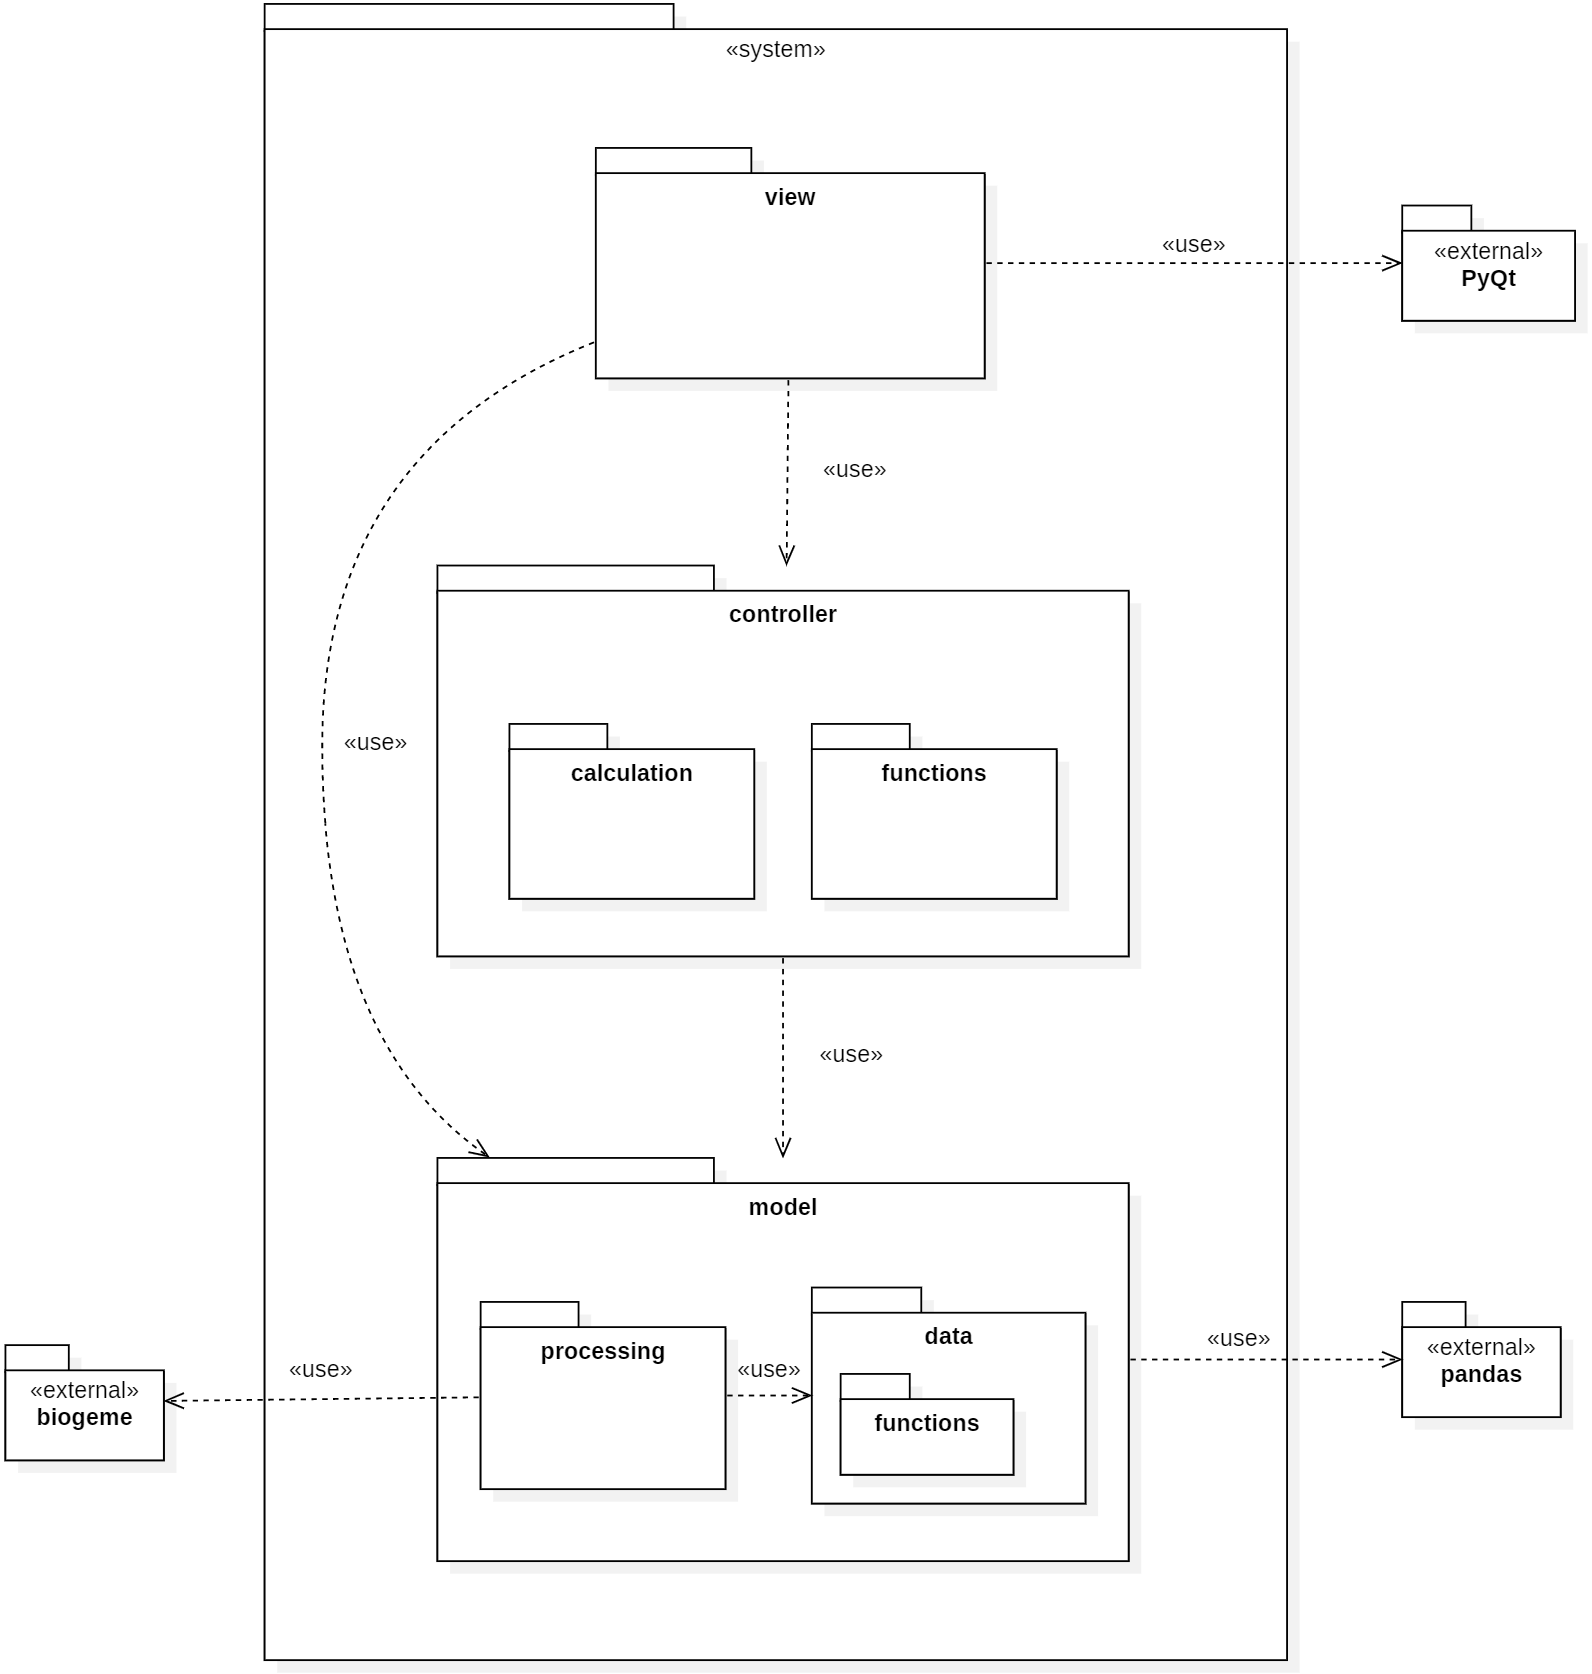
\includegraphics[width=13cm]{img/PackageDiagram.png}
    \caption{Paketdiagramm}
\end{figure}

\begin{itemize}
\item Die Software wird nach dem Prinzip der MVC-Architektur entworfen und setzt sich zusammen aus der View, dem Controller und dem Model.
\end{itemize}

\subsection{View}
\begin{itemize}
\item Die View ist verantwortlich für die visuelle Präsentation der im Model vorhandenen Daten. Dafür greift die View auf das externe Paket \textit{\textbf{PyQt}} zu. Dies wird für die Erstellung der graphischen Benutzeroberfläche verwendet.
\item Nutzereingaben werden immer über den \textbf{Controller} weitergeleitet. Somit kann eine schwache Kopplung zum \textbf{Model} beibehalten werden.
\item Da die View auf Erweiterungen des \textbf{Models} reagieren muss, kann eine Abhängigkeit allerdings nicht vermieden werden.
\end{itemize}

\subsection{Controller}
\begin{itemize}
\item Die Controller sind dafür zuständig, die Nutzereingaben aus der View an das Model weiterzuleiten.
\item Finden Änderungen im Model statt, so senden die betroffenen Klassen der View \emph{update}-Aufrufe über die Controller aus. Dabei werden die betroffenen Daten aus dem Model zurückgegeben.
\item \textbf{Calculation-Paket}: Enthält Controller, die bei der Konfiguration der Berechnung oder beim Umgang mit dem Ergebnis aufgerufen werden.
\item \textbf{Functions-Paket}: Controller, die zum Bearbeiten von Alternativen und
Attributsableitungen aufgerufen werden.
\end{itemize}

\subsection{Model}
\begin{itemize}
\item Das Model umfasst die Datenhaltung und Manipulation dieser Daten bei einem geöffneten Projekt.
\item Bei Änderungen ist das Model zudem verantwortlich vergangene Eingaben zu speichern. Diese sollen anhand einer undo-/redo-Funktion wieder aufrufbar sein.
\item Das externe Python Paket \emph{\textbf{pandas}} wird für die Haltung tabellarischer, vom Nutzer nicht veränderbarer Daten verwendet.
\item \textbf{Processing-Paket}: Umschließt die Funktionalität, welche die Konfiguration der Berechnung oder das Ergebnis betrifft. Es existiert eine Schnittstelle, über welche die tatsächliche Berechnung stattfinden kann. Hier wird standardmäßig das externe Python Paket \emph{\textbf{biogeme}} verwendet.
\item \textbf{Data-Paket}: Umfasst jegliche Funktionalität, die für die Datenhaltung und Änderung des Verkehrsmodells zuständig ist.
\item \textbf{Functions-Paket}: Unterpaket von \textbf{Data}. Umfasst spezifisch den Teil des Modells, in welchem die Ausdrücke und Funktionen der Attributsableitungen und Alternativen gehandhabt werden.
\end{itemize}

\newpage
\section{Klassenstruktur}
Im folgenden Abschnitt werden die einzelnen Klassen des Entwurfs dokumentiert, aufgeteilt nach den Paketen. Das gesamte Klassendiagramm, indem die Klassen aller Pakete gemeinsam abgebildet sind, befindet sich im Anhang (vgl Abb. ~\ref{fig:CompleteClassDiagram}). In diesem Kapitel sind alle genannten Attribute \emph{private} und alle Methoden \emph{public} soweit nicht explizit anders angegeben. Triviale Funktionen wie einfache \emph{get} und \emph{set} Methoden, sowie triviale Konstruktoren werden nicht genannt.

\subsection{View}
\begin{figure}[H]%
    \centering
    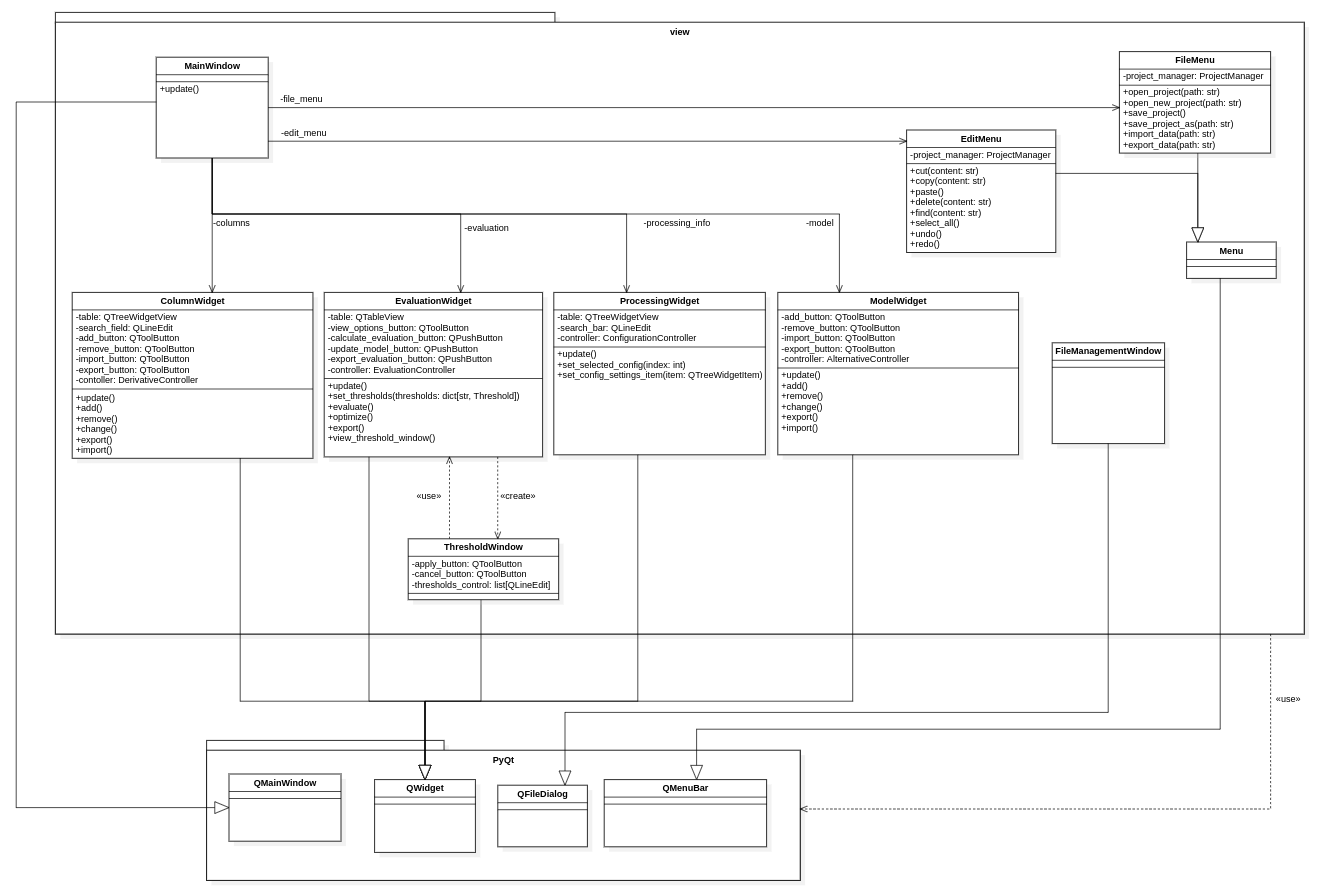
\includegraphics[width=13cm]{entwurf/Entwurf_dokument/img/Alissa/ViewUpdated.png}
    \caption{Das Paket View und seine Klassen}
    \label{fig:classDiagrammView}
\end{figure}
In Abb. ~\ref{fig:classDiagrammView} ist das Paket der View mit allen ihren Klassen abgebildet, ebenso wie die relevanten Klassen des Pakets \emph{PyQt}.
Im der View sind alle Funktionalitäten enthalten, die zur Realisierung der GUI beitragen. Für die graphische Schnittstelle wird \emph{PyQt} benutzt. Aus diesem Grund erben die Klassen in der View ihre Funktionalität und Struktur aus den Klassen des \emph{PyQt} Pakets. Im Folgenden erfolgt die Beschreibung und Erklärung der einzelnen Klassen.

\newpage

\classheader[]{MainWindow}\label{cls:MainWindow}
\begin{tabular}{lll}
 Superklassen: & \href{https://doc.qt.io/qt-6/qmainwindow.html}{QMainWindow}\\
\end{tabular}\\

\begin{figure}[H]%
    \centering
    \begin{minipage}[b]{0.4\textwidth}
        \centering
        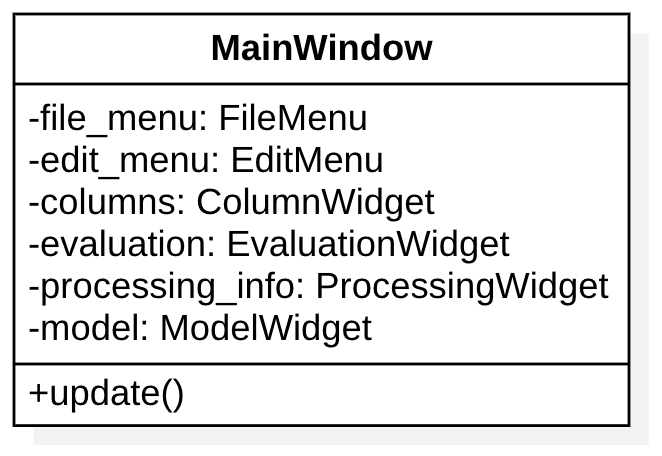
\includegraphics[width=5cm]{entwurf/Entwurf_dokument/img/klassenView/MainWindow.png}
        \caption{Die Klasse MainMenu}
    \end{minipage}
    \hfill
    \begin{minipage}[b]{0.4\textwidth}
        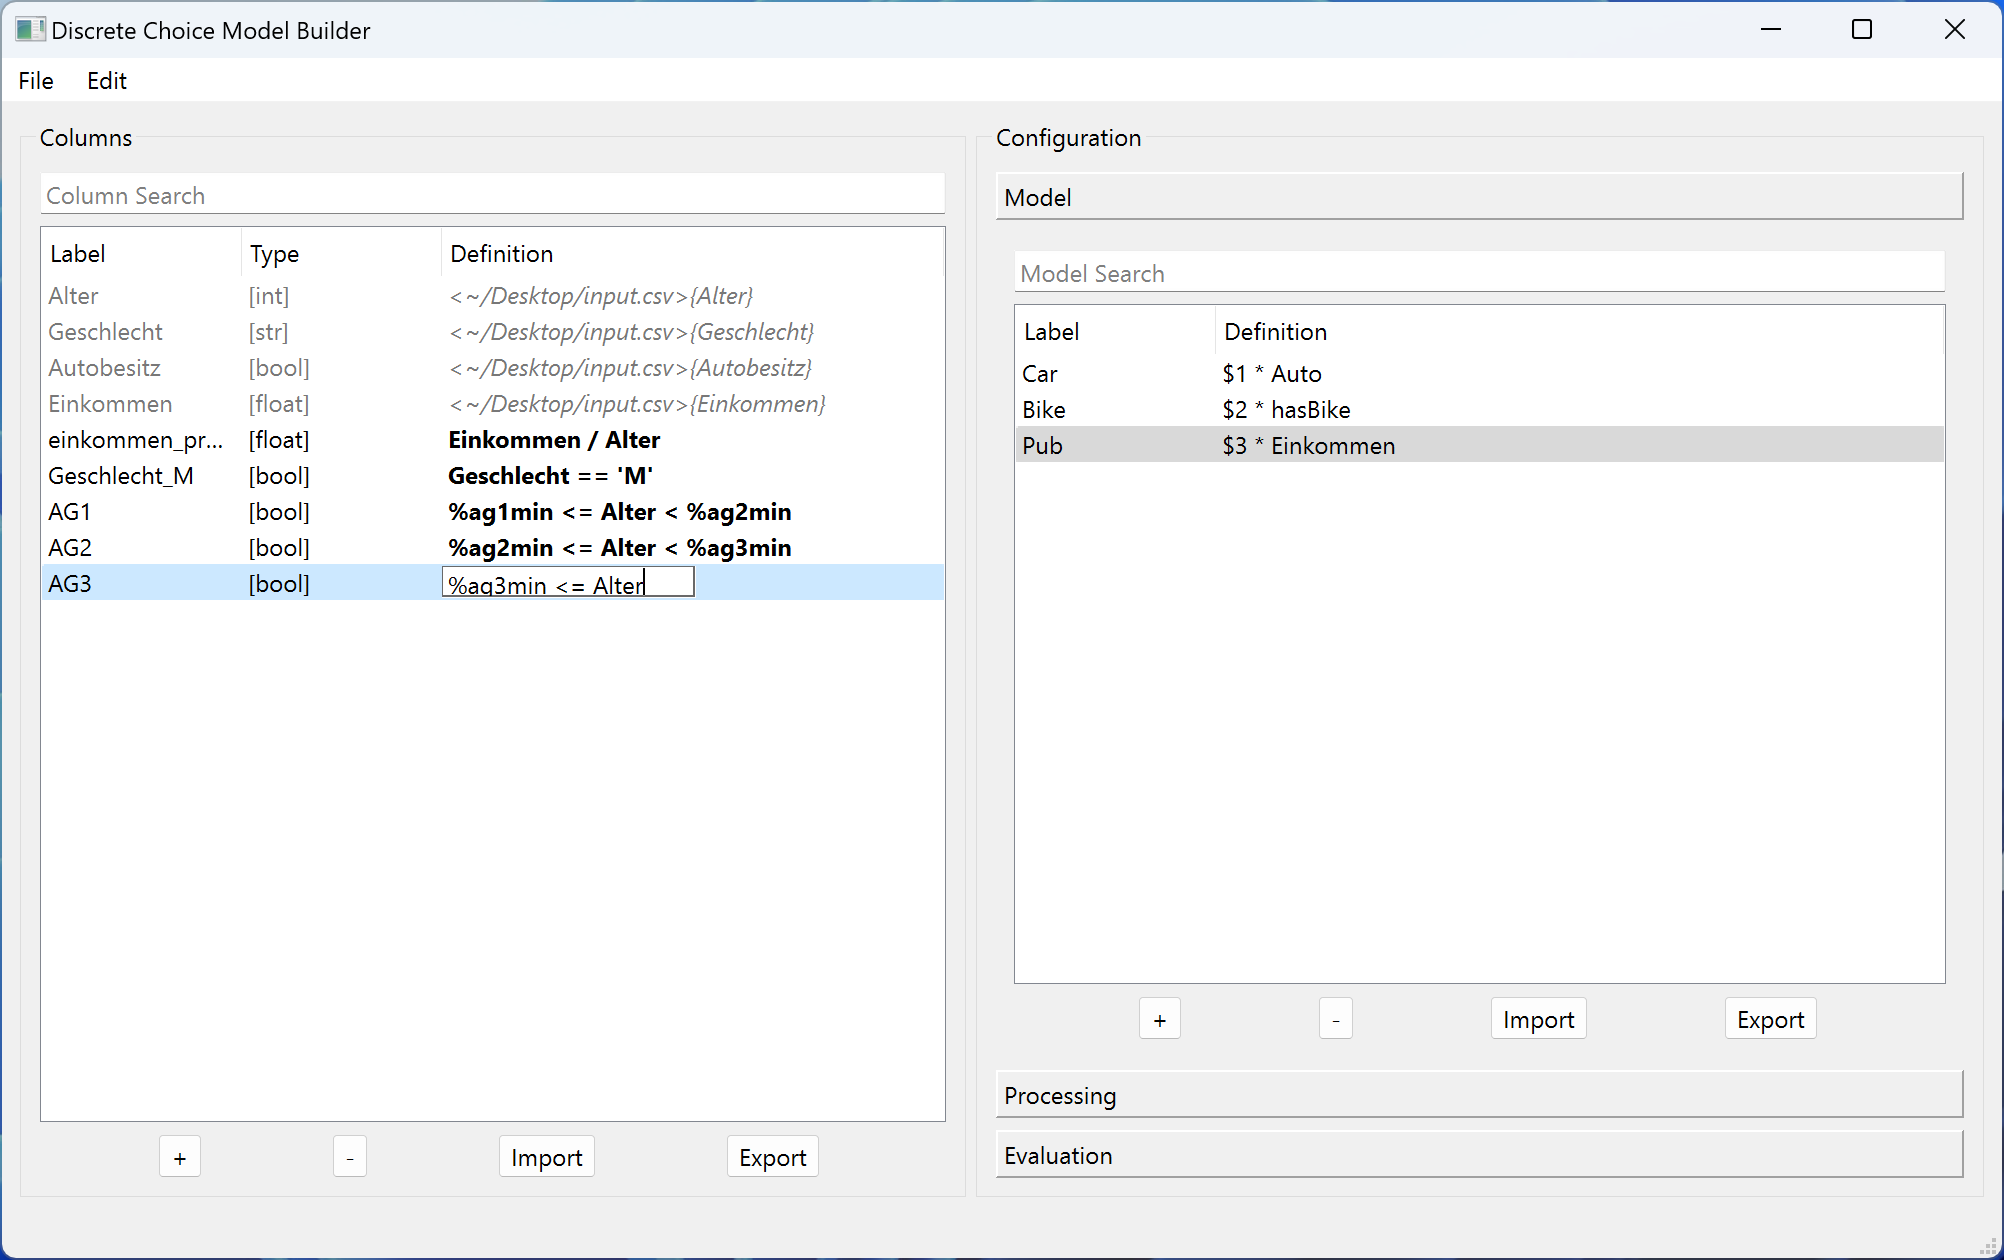
\includegraphics[width=8cm]{specifications/img/gui-screenshots/columns-editing+model.png}
        \caption{Graphisches Beispiel für das Hauptfenster}
        \label{fig:guiMainWindow}
    \end{minipage}
\end{figure}
Die Klasse MainWindow repräsentiert das Hauptfenster (vgl Abb. ~\ref{fig:guiMainWindow}). In dem befinden sich alle graphischen Elemente (Bspw. Tabellen, Menüs, Knöpfe usw.). Die einzelnen Elemente werden je in ihrer eigenen Klasse spezifiziert. Dies erleichtert die Refaktorisierung und das nachträgliche Hinzufügen neuer graphischen Elemente.
\\\\

\textbf{{Attribute}}
\begin{itemize}
\item \texttt{file\char`_menu: FileMenu} \newline Repräsentiert das Dateimenü in der GUI.
\item \texttt{edit\char`_menu: EditMenu} \newline Repräsentiert das Editmenü in der GUI.
\item \texttt{columns: ColumnWidget} \newline Repräsentiert die Tabelle mit Erhebungsdaten und Ableitungen. In der GUI befindet sie sich links im Hauptfenster.
\item \texttt{evaluation: EvaluationWidget} \newline Repräsentiert das Teilfenster, in dem die Ergebnisse der Berechnungen gezeigt werden.
\item \texttt{processing\char`_info: ProcessingWidget} \newline Repräsentiert den Abschnitt aus der GUI, in dem die ausgewählte Konfiguration und deren Variablen angezeigt werden.
\item \texttt{model: ModelWidget} \newline Steht für den Abschnitt \textit{Model}, in dem die Alternativen zu sehen sind.
\end{itemize}

\textbf{{Methoden}}
\begin{itemize}
\item \texttt{update()} \newline Dient zur Aktualisierung der GUI, wenn ein Befehl aus dem Dateimenü oder Editmenü ausgefüht wird und dies die angezeigten Daten ändert. Ein Beispiel is das Importieren von Erhebungsdaten, nachdem diese in der Ansicht angezeigt werden müssen.
\end{itemize}

\newpage
\classheader[]{Menu}\label{cls:Menu}
\begin{tabular}{lll}
 Superklassen: & \href{https://doc.qt.io/qtforpython-5/PySide2/QtWidgets/QMenuBar.html}{QMenuBar}\\
 Subklassen: & \hyperref[cls:FileMenu]{FileMenu}, \hyperref[cls:EditMenu]{EditMenu}
\end{tabular}\\
\begin{figure}[H]%
    \centering
    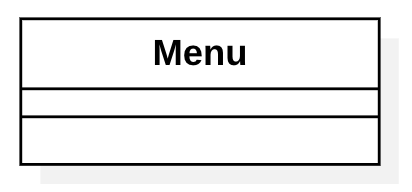
\includegraphics[width=4cm]{entwurf/Entwurf_dokument/img/klassenView/Menu.png}
    \caption{Die Klasse Menu}
\end{figure}
Die Klasse Menu steht für ein Menü in der Menüleiste. Die einzelnen Menüs haben gemeinsame Eigenschaften, wie z.B. eine gleiche Struktur, aber jedes Menü bietet dem Nutzer unterschiedliche Operationen. Aus diesem Grund wird für jedes spezielle Menü eine eigene Klasse erstellt.
\\\\
\newpage
\classheader[]{FileMenu}\label{cls:FileMenu}
\begin{tabular}{lll}
 Superklassen: & \hyperref[cls:Menu]{Menu}\\
\end{tabular}\\
\begin{figure}[H]%
    \centering
    \begin{minipage}[b]{0.4\textwidth}
        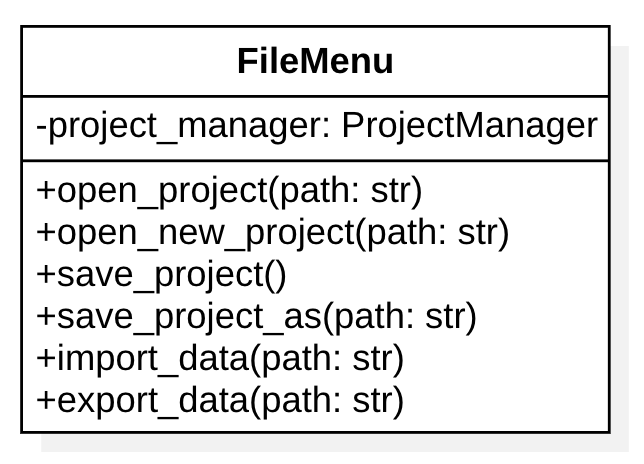
\includegraphics[width=5cm]{entwurf/Entwurf_dokument/img/klassenView/FileMenu.png}
        \caption{Die Klasse FileMenu}
    \end{minipage}
    \hfill
    \begin{minipage}[b]{0.4\textwidth}
        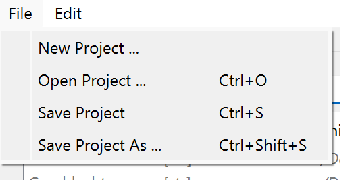
\includegraphics[width=6cm]{entwurf/Entwurf_dokument/img/Alissa/EditMenuGUI.png} %Aus versehen anders benannt. Sollte eig. FileMenuGUI heißen
    \caption{Graphisches Beispiel für das Dateimenü}
    \label{fig:FileMenuGUI}
    \end{minipage}
\end{figure}
Die Klasse FileMenu ist die Realisierung des Dateimenüs aus der graphischen Schnittstelle (vgl Abb. ~\ref{fig:FileMenuGUI}). Sie erbt ihre Struktur von der Klasse \textit{Menu}. Die Klasse \textit{FileMenu} bietet dem Nutzer die Möglichkeit, das Projekt zu verwalten durch Funktionen wie Import oder Speicherung.
\newline \newline

\textbf{{Attribute}}
\begin{itemize}
\item \texttt{project\char`_manager: ProjectManager} \newline Der Controller, der für die Verwaltung des Projekts zuständig ist.
\end{itemize}

\textbf{{Methoden}}
\begin{itemize}
\item \texttt{open\char`_project(path:str)} \newline Diese Methode ermöglicht dem Nutzer, ein bereits existierendes Projekt zu öffnen.
\\\\
\underline{{Parameter}}\\
\begin{tabular}{lll}
 & \texttt{path} & Der Dateipfad, an dem das Projekt gespeichert ist. \\
\end{tabular}

\item \texttt{open\char`_new\char`_project(path:str)} \newline Ermöglicht dem Nutzer, ein neues Projekt zu öffnen.
\\\\
\underline{{Parameter}}\\
\begin{tabular}{lll}
 & \texttt{path} & Der Dateipfad, an dem das Projekt geöffnet und gespeichert werden soll. \\
\end{tabular}

\item \texttt{save\char`_project()} \newline Ermöglicht dem Nutzer, das geöffnete Projekt zu speichern. Der Pfade der Speicherung ist bereits als Attribut im Projekt enthalten.


\item \texttt{save\char`_project\char`_as(path:str)} \newline Durch diese Methode kann der Nutzer das geöffnete Projekt, an einem anderen Dateipfad speichern.
\\\\
\underline{{Parameter}}\\
\begin{tabular}{lll}
 & \texttt{path} & Der Dateipfad, wo das Projekt gespeichert werden soll. \\
\end{tabular}


\item \texttt{import\char`_data(path:str)} \newline Zum Laden einer CSV-Datei mit den Erhebungsdaten.
\\\\
\underline{{Parameter}}\\
\begin{tabular}{lll}
 & \texttt{path} & Der Dateipfad, wo sich die CSV-Datei befindet.\\
\end{tabular}


\item \texttt{export\char`_data(path:str)} \newline Mit dieser Methode, kann die Tabelle mit den Erhebungsdaten und Ableitungen als CSV-Datei exportiert werden.
\\\\
\underline{{Parameter}}\\
\begin{tabular}{lll}
 & \texttt{path} & Der Dateipfad, wo die exportierte CSV-Datei gespeichert wird. \\
\end{tabular}
\end{itemize}

\newpage
\classheader[]{EditMenu}\label{cls:EditMenu}
\begin{tabular}{lll}
 Superklassen: & \hyperref[cls:Menu]{Menu}\\
\end{tabular}\\
\begin{figure}[H]%
    \centering
    \begin{minipage}[b]{0.4\textwidth}
        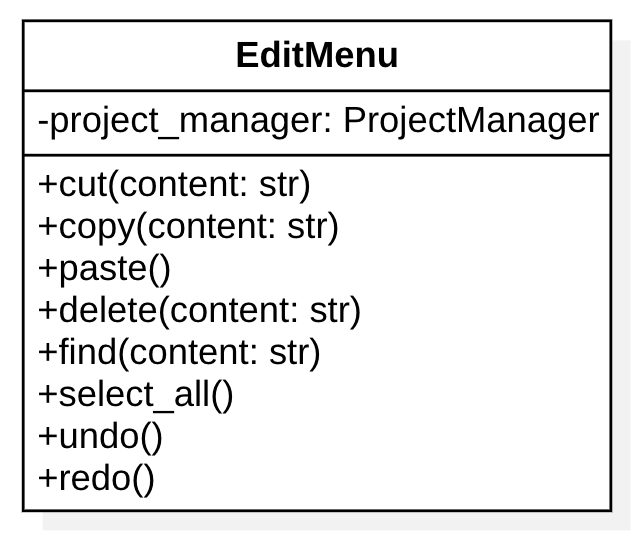
\includegraphics[width=5cm]{entwurf/Entwurf_dokument/img/klassenView/EditMenu.png}
        \caption{Die Klasse EditMenu}
    \end{minipage}
    \hfill
    \begin{minipage}[b]{0.4\textwidth}
        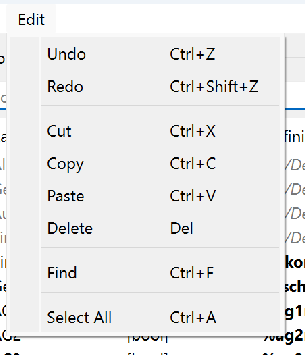
\includegraphics[width=6cm]{entwurf/Entwurf_dokument/img/Alissa/FileMenuGUI.png} %Aus versehen anders benannt. Sollte eig. EditMenuGUI heißen
        \caption{Graphische Darstellung von dem Editmenü}
        \label{fig:EditMenuGUI}
    \end{minipage}
\end{figure}
Die Klasse \textit{EditMenu} repräsentiert das Editmenü des GUI (vgl Abb. ~\ref{fig:EditMenuGUI}. Sie erbt von der Klasse \textit{Menu} und bietet dem Nutzer Operationen, um die Arbeit mit dem Projekt durch Shortcuts effizienter zu gestalten. Es enthält Standardoperationen wie \emph{Copy}, \emph{Cut}, \emph{Paste}, \emph{Delete} und \emph{Select All}, die dem Nutzer Arbeit durch erneutes Eingeben oder einzelnes Löschen von Text ersparen soll. Ebenfalls dienen die Funktionen \textit{undo} und \textit{redo} der Bedienbarkeit der Software, und sind integraler Bestandteil des Entwurfs.
\newline \newline
\textbf{{Attribute}}
\begin{itemize}
\item \texttt{project\char`_manager: ProjectManager} \newline Der Controller, der für das Projekt Managment verantwortlich ist. Über ihn erfolgt der Zugriff auf das Projekt.
\end{itemize}

\textbf{{Methoden}}
\begin{itemize}
\item \texttt{undo()} \newline Die zuletzt ausgeführte Aktion wird rückgängig gemacht. Kann nur angewandt werden falls breits Aktionen ausgeführt wurden.

\item \texttt{redo()} \newline Das Wiederherstellen der zuletzt rückgängig gemachten Operation. Kann nur angewandt werden wenn die letzte ausgeführte Aktion das Rückgängigmachen einer Aktion war.

\item \texttt{cut(content: str)} \newline Einen ausgewählten Text ausschneiden. Der Ausgewählte Text wird in die Zwischenablage kopiert und aus der Nutzereingabe entfernt. Diese Operation kann nur in Textfeldern angewandt werden, die für Nutzereingaben bestimmt sind. Diese Methode ist eine Implementierung der gleichnamigen Methode der Klasse XY.
\\\\
\underline{{Parameter}}\\ 
\begin{tabular}{lll}
 & \texttt{content} & Der Inhalt zum Ausschneiden\\
\end{tabular}

\item \texttt{copy(content:str} \newline Ausgewählten bzw. markierten Text in die Zwischenablage kopieren.
\\\\
\underline{{Parameter}}\\
\begin{tabular}{lll}
& \texttt{content} & Bezeichnet den zu kopierenden Inhalt \\
\end{tabular}

\item \texttt{paste()} \newline Den Text der sich aktuell in der Zwischenablage befindet an die ausgewählte Stelle einsetzen. Vorraussetzungen für diese Funktion ist, dass sich Text in der Zwischenablage befindet und die von Nutzer ausgewählte Stelle in einem Text Eingabefeld ist.

\item \texttt{delete(content: str)} \newline Einen vom Nutzer ausgewählten Text löschen. Diese Methode kann nur auf Text angewandt werden, der sich in einem Texteingabefeld befindet.
\\\\
\underline{{Parameter}}\\ 
\begin{tabular}{llp{8.7cm}}
&\texttt{content} & Der ausgewählte Text, der gelöscht werden soll. Dieser muss sich in einem Texteingabefeld befinden.\\
\end{tabular}

\item \texttt{find(content:str)} \newline Einen vom Nutzer bestimten Text im Hauptfenster finden. Der Text wird in der gesamten Ansicht des Hauptfensters, also allen sichtbaren Tabellen der Attributsableitungen, Alternativen oder Auswertung, gesucht.
\\\\
\underline{{Parameter}}\\
\begin{tabular}{lll}
 & \texttt{content} & Der Inhalt, wonach gesucht werden soll. \\
\end{tabular}

\item \texttt{select\char`_all()} \newline Alles auswählen, was im ausgewählten Textfeld der betrachteten Tabelle existiert.
\end{itemize}

\newpage
\classheader[]{FileManagmentWindow}\label{cls:FileManagmentWindow}
\begin{tabular}{lll}
 Superklassen: & \href{https://doc.qt.io/qtforpython-5/PySide2/QtWidgets/QFileDialog.html}{QFileDialog}\\
\end{tabular}\\
\begin{figure}[H]%
    \centering
    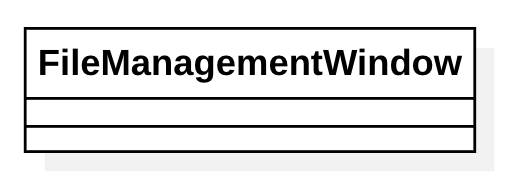
\includegraphics[width=5cm]{entwurf/Entwurf_dokument/img/klassenView/FileManagementWindow.png}
    \caption{Die Klasse \textit{FileManagmentWindow}}
\end{figure}
Die Klasse \textit{FileManagmentWindow} repräsentiert den Datei-Dialog. Das Fenster, womit der Nutzer die Dateien (CSV oder JSON) aussuchen und auswählen kann. Diese Klasse erbt von \textit{QFileDialog}, dessen Informationen sind in den \href{https://doc.qt.io/qtforpython-5/PySide2/QtWidgets/QFileDialog.html}{PyQt Docs} zu finden. Die Klassen \textit{QFileDialog} implementiert alle notwendigen Funktionen des Datei-Dialogs. Die Kindesklasse \textit{FileManagmentWindow} benötigt daher keine spezielle Eigenschaften, weswegen keine neue Methoden oder Attribute hinzukommen. Die Existenz dieser Klasse ist notwendig und eine Erweiterung des Datei Managements um Funktionen , die nicht on PyQt implementiert wurden, zu erlauben


\newpage
\classheader[]{ColumnWidget}\label{cls:ColumnWidget}
\begin{tabular}{lll}
 Superklassen: & \href{https://doc.qt.io/qt-6/qwidget.html}{QWidget}\\
\end{tabular}\\
\begin{figure}[H]%
    \centering
    \begin{minipage}[b]{0.4\textwidth}
        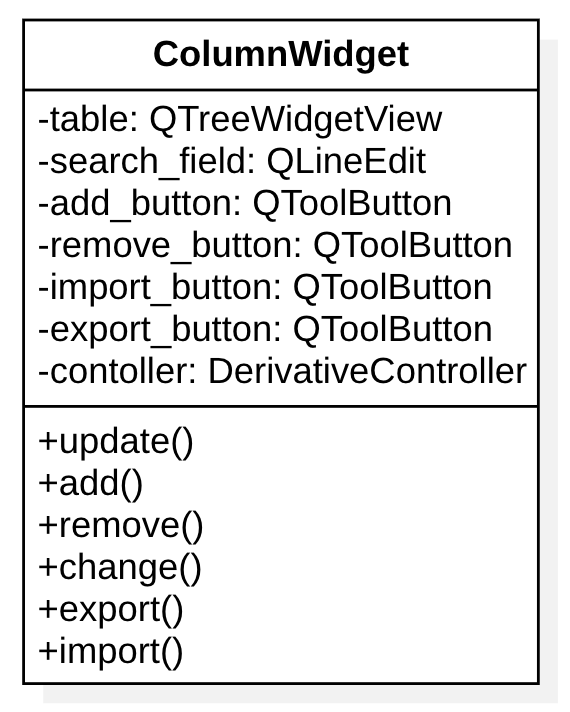
\includegraphics[width=5cm]{entwurf/Entwurf_dokument/img/klassenView/ColumnWidget.png}
        \caption{Die Klasse ColumnWidget}
    \end{minipage}
    \hfill
    \begin{minipage}[b]{0.4\textwidth}
        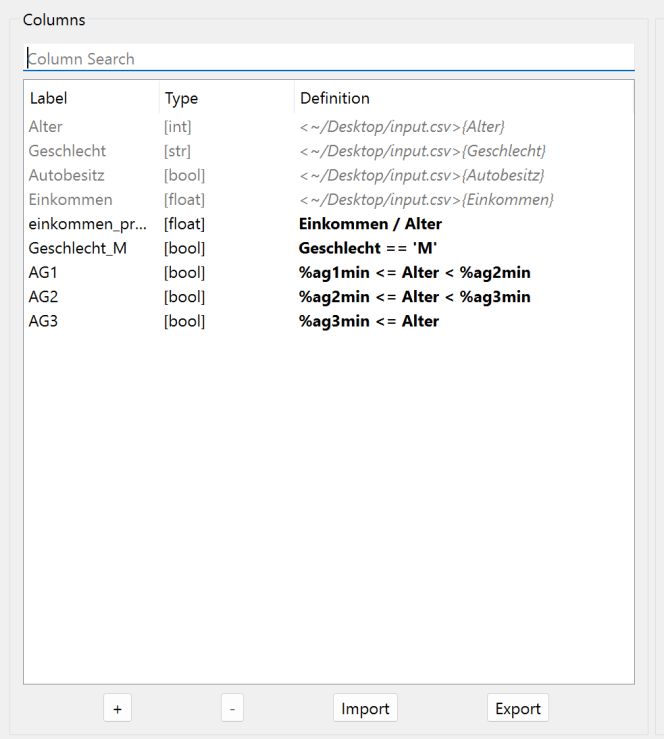
\includegraphics[width=5cm]{entwurf/Entwurf_dokument/img/Alissa/Columns.png} 
    \caption{Der Columns-Abschnitt im GUI.}
    \label{fig:ColumnsGUI}
    \end{minipage}
\end{figure}
\textit{ColumnWidget} repräsentiert die Tabelle in der GUI, wo die Spalten aus den Erhebubgsdaten und den Attributsableitungen gezeigt werden (vgl Abb. ~\ref{fig:ColumnsGUI}). Außerdem erbt diese Klasse von QWidget aus der PyQt Biblothek. Das ist die Basis Klasse für alle Objekte, die Nutzerinterktion ermöglichen. Weiter Informationen sind auf \href{https://doc.qt.io/qt-6/qwidget.html}{PyQt Docs} zu finden.
\newline 

\textbf{{Attribute}}
\begin{itemize}
\item \texttt{table: QTreeWidgetView} \newline Beinhaltet die Tabelle mit den Attributen.
\item \texttt{search\char`_field: QLineEdit} \newline Repräsentiert das Suchfeld. In der GUI ist dies oberhalb der Tabelle \textit{table} (vgl Abb. ~\ref{fig:ColumnsGUI}).
\item \texttt{add\char`_button: QToolButton} \newline Damit wird die \textit{add "+"} Schaltfläche realisiert, womit der Nutzer ein Attribut hinzufügen kann.
\item \texttt{remove\char`_button:QToolButton} \newline Steht für die \textit{remove "\textendash"} Schaltfläche. Mit dem kann der Nutzer eine ausgewählte Attributsableitung entfernen. 
\item \texttt{import\char`_button: QToolButton} \newline Diese Schaltfläche emöglicht dem Nutzer Attributsableitungen zu importieren.
\item \texttt{export\char`_button: QToolButton} \newline Mit dieser Schlatfläche kann der Nutzer ausgewählte Attributsableitungen exportieren (als CSV oder JSON).
\item \texttt{controller: DerivativeController} \newline Der Controller, mit dem die Nutzeranfragen bzgl. der Verwaltung von Attributsableitungen umgesetzt werden. Er ist die Schnittstelle zum Teil 'Control' des MVC Entwurfsmusters.
\end{itemize}

\textbf{{Methoden}}
\begin{itemize}
\item \texttt{update()} \newline Aktualisiert die Anzeige sobald Änderungen am Model vorgenommen wurden und bspw. Fehler wurde bei der Eingabe erkannt und hervorgehoben werden müssen. Diese Methode ist dafür verantwortlich mit dem zuständigen Controller zu kommunizieren und von diesem die Daten aus dem Model zu erhalten.

\item \texttt{add()} \newline Gibt dem Nutzer die Möglichkeit, in der Tabelle eine Attributsableitung hinzuzufügen.

\item \texttt{remove()} \newline Gibt dem Nutzer die Möglichkeit, in der Tabelle eine ausgewählte Attributsableitung zu löschen

\item \texttt{change()} \newline Mit dieser Funktion wird das Ändern einer Attributsableitung ermöglicht.

\item \texttt{export()} \newline Ist zuständig für das Exportieren von Attributsableitungen.

\item \texttt{import()} \newline Steht für das Importieren von Attributsableitungen.
\end{itemize}

\newpage
\classheader[]{EvaluationWidget}\label{cls:EvaluationWidget}
\begin{tabular}{lll}
 Superklassen: & \href{https://doc.qt.io/qt-6/qwidget.html}{QWidget}\\
\end{tabular}\\
\begin{figure}[H]%
    \centering
    \begin{minipage}[b]{0.4\textwidth}
        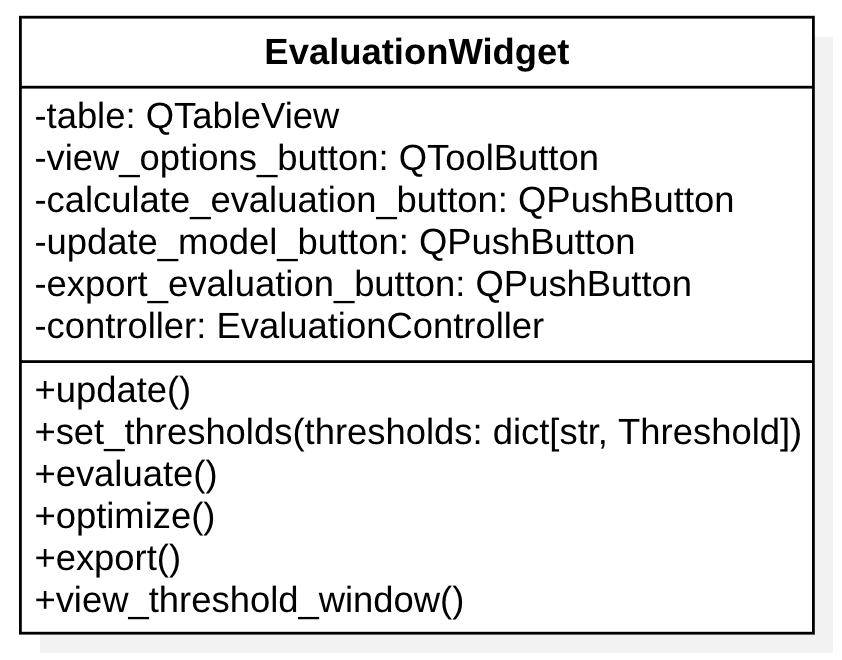
\includegraphics[width=5cm]{entwurf/Entwurf_dokument/img/klassenView/EvaluationWidget.png}
        \caption{Die Klasse EvaluationWidget}
    \end{minipage}
    \hfill
    \begin{minipage}[b]{0.4\textwidth}
        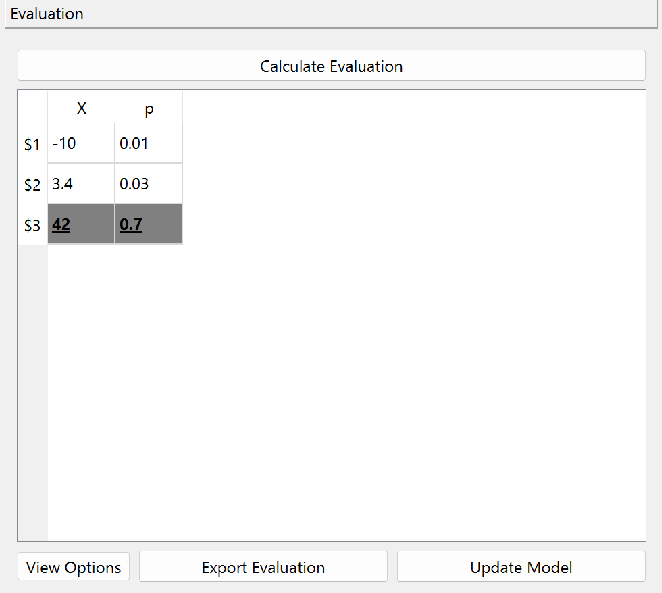
\includegraphics[width=5cm]{entwurf/Entwurf_dokument/img/Alissa/evaluationGUI.png} 
    \caption{Der \textit{Evaluation}-Abschnitt im GUI.}
    \end{minipage}
\end{figure}
Die Klasse \textit{EvaluationWidget} enthält alle benötigten Eigenschaften und Methoden, damit die Tabelle der Auswertung realisiert wird.
\newline

\textbf{{Attribute}}
\begin{itemize}
\item \texttt{table: QTableView} \newline Tabelle, welche die Ergebnisse der Auswertung enthält.
\item \texttt{view\char`_options\char`_button: QToolButton} \newline Zeigt das Fenster, wo der Nutzer den Schwellwert ändern kann.
\item \texttt{calculate\char`_evaluation\char`_button:  QPushButton} \newline Das ist die Schaltfläche, mit dem das Auswerten betätigt wird.
\item \texttt{update\char`_model\char`_button:QPushButton} \newline  Button mit der Nutzer das Model optimieren kann.
\item \texttt{export\char`_evaluation\char`_button:  QPushButton} \newline Ermöglicht dem Nutzer, die Ergebnisse der Auswertung zu exportieren.
\item \texttt{controller: EvaluationController} \newline Der Controller, worüber mit dem Model kommuniziert wird, um die Nutzeranfragen bzgl. der Auswertung und Optimierung umzusetzen.
\end{itemize}

\textbf{{Methoden}}
\begin{itemize}
\item \texttt{update()} \newline Aktualisiert die Nutzeranzeige, wenn was am Model geändert wird, bspw nachdem die Schwellwertänderung erfolgreich umgesetzt wurde werden mit dieser Methode die Schwellwerte aus dem Modell geholt und angezeigt.

\item \texttt{set\char`_thresholds(thresholds: dict[str, Threshold])} \newline Fügt dieübergebenen Schwellwerte in das Projekt ein.
\\\\
\underline{{Parameter}}\\ 
\begin{tabular}{lp{10.7cm}}
 & \texttt{thresholds: dict[str, Threshold]} Sammlung von Schwellwerten, die eingefügt werden müssen. Die Schlüssel im Dictionary sind die Bezeichner der Schwellerte und die Threshold-Instanzen, die vom ThresholdWindow verarbeiteten Werte.\\
\end{tabular}

\item \texttt{evaluate()} \newline Die Methode startet die Ausführung der Auswertung im Modell.

\item \texttt{optimize()} \newline Startet die Optimierung des Modells.

\item \texttt{export()} \newline Exportiert die Ergebnisse der Auswertung. 

\item \texttt{view\char`_threshold\char`_window()} \newline Zeigt dem Nutzer das Fenster, wo er die Schwellwerte eingeben und anwenden kann. Hierfür wird ein Objekt der Klasse \textit{ThresholdWindow} erstellt.
\end{itemize}

\newpage
\classheader[\flqq{}setereotype\frqq]{ThresholdWindow}\label{cls:ThresholdWindow}
\begin{tabular}{lll}
 Superklassen: & \href{https://doc.qt.io/qt-6/qwidget.html}{QWidget}\\
 Subklassen: & --\\
\end{tabular}\\
\begin{figure}[H]%
    \centering
    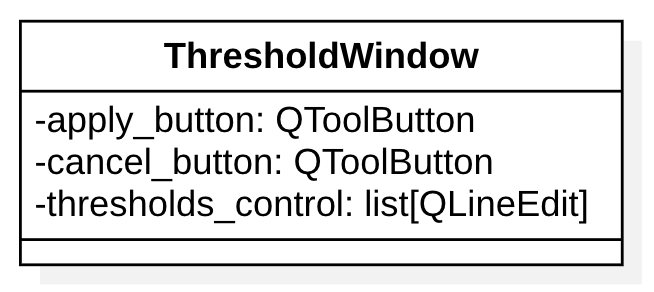
\includegraphics[width=5cm]{entwurf/Entwurf_dokument/img/klassenView/ThresholdWindow.png}
    \caption{Die Klasse \textit{ThresholdWidget}}
\end{figure}
Diese Klasse repräsentiert das Fenster, wo der Nutzer die Schwellwerte eingeben und anwenden kann. Die Klasse nutzt die Methode \texttt{set\char`_thresholds(thresholds: dict[str, Threshold])} aus der Klasse \textit{EvaluationWindow}, um die Schwellwerte anzuwenden.
\newline \newline

\textbf{{Attribute}}
\begin{itemize}
\item \texttt{apply\char`_button: QToolButton} \newline Die Schaltfläche, womit der Nutzer das Anwenden der Schwellwerte betätigen kann. Mit dem Anwenden eines Schwellwertes ist gemeint, dass dieser im Projekt hinterlegt wird und nach erfolgter Evaluierung zur Visualisierung verwendet wird.

\item \texttt{cancle\char`_button: QToolButton} \newline Die Schaltfläche, womit der Nutzer den Vorgang abbricht und zurück zum Hauptfenster geleitet wird. Wird dieser Button betätigt werden vom Nutzer betätigte Eingaben im ThresholdWindow verworfen.

\item \texttt{thresholds\char`_control: list[QLineEdit]} \newline Liste von den Schwellwerten, die der Nutzer verändern kann.
\end{itemize}

\newpage
\classheader[\flqq{}setereotype\frqq]{ProcessingWidget}\label{cls:ProcessingWidget}
\begin{tabular}{lll}
 Superklassen: & \href{https://doc.qt.io/qt-6/qwidget.html}{QWidget}\\
\end{tabular}\\
\begin{figure}[H]%
    \centering
    \begin{minipage}[b]{0.4\textwidth}
        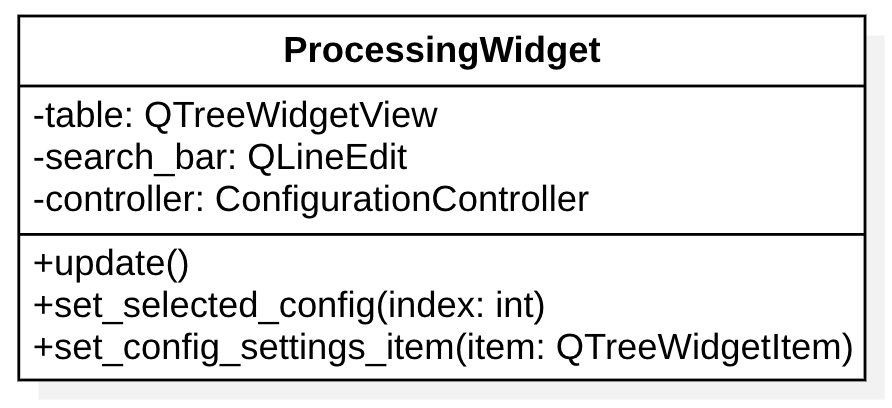
\includegraphics[width=5cm]{entwurf/Entwurf_dokument/img/klassenView/ProcessingWidget.png}
        \caption{Die Klasse \textit{ProcessingWidget}}
    \end{minipage}
    \hfill
    \begin{minipage}[b]{0.4\textwidth}
        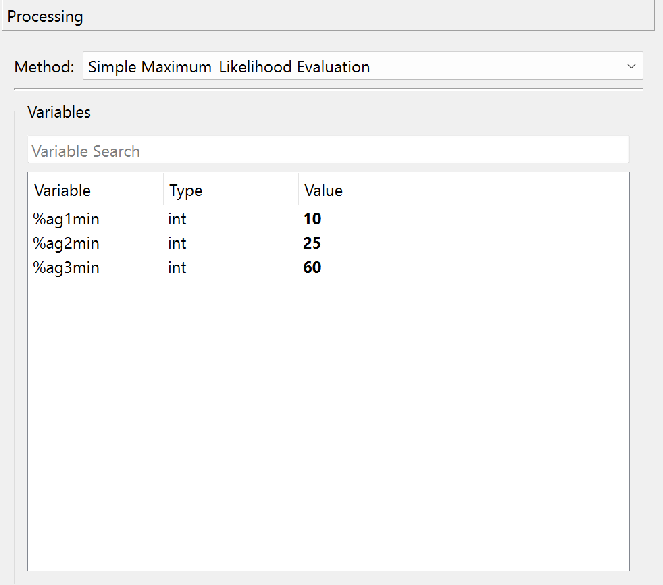
\includegraphics[width=5cm]{entwurf/Entwurf_dokument/img/Alissa/Processing.png} 
    \caption{Die \textit{Processing}-Abschnitt in der GUI.}
    \label{fig: ProcessingWidgetGUI}
    \end{minipage}
\end{figure}
Die Klasse \textit{ProcessingWidget} repräsentiert das Processing Fenster in der GUI, in dem der Nutzer die Methode für die Auswertung wählen kann (vgl Abb. ~\ref{fig: ProcessingWidgetGUI}. Diese Klasse erbt von der Klasse \textit{QWidget} aus dem Paket PyQt. Weitere Informationen bezüglich der Klasse QWidget sind in der \href{https://doc.qt.io/qt-6/qwidget.html}{Dokementation} zu finden.
\newline \newline

\textbf{{Attribute}}
\begin{itemize}
\item \texttt{table: QTreeWidget} \newline Steht für die Tabelle in der GUI, wo der Nutzer die Variablen sehen kann.
\item \texttt{search\char`_bar: QLineEdit} \newline Steht für das Suchfeld mit dem der Nutzer nach Variablen suchen kann.
\item \texttt{controller: ConfigurationController} \newline Das ist der Controller, der Nutzeranfragen im Processing Fenster verarbeitet und als Schnittstelle zum Model dient.
\end{itemize}

\textbf{{Methoden}}
\begin{itemize}
\item \texttt{update()} \newline Operation aktualisiert die Anzeige für en Nutzer, falls was an der Tabelle geändert wurde.

\item \texttt{change\char`_processing\char`_config(index: int)} \newline Ändert die Konfiguration für die Berechnungen.
\\\\
\underline{{Parameter}} \\
\begin{tabular}{lp{10.7cm}}
&\texttt{index: int} Der Index der Konfiguration, die aus der vorliegenden Liste an möglichen Konfigurationen ausgewählt wurde.\\
\end{tabular}


\item \texttt{set\_config\_settings\_item(item: QWidgetItem)} \newline Ändert die Variablen der ausgewählten Konfiguration.
\\\\
\underline{{Parameter}} \\
\begin{tabular}{lp{10.7cm}}
&\texttt{item: QWidgetItem} Das Widget, in dem sich die veränderten Parameter der Konfiguration befinden.\\
\end{tabular}

\end{itemize}

\newpage
\classheader[]{ModelWidget}\label{cls:ModelWidget}
\begin{tabular}{lll}
 Superklassen: &\href{https://doc.qt.io/qt-6/qwidget.html}{QWidget}\\
\end{tabular}\\
\begin{figure}[H]%
    \centering
    \begin{minipage}[b]{0.4\textwidth}
        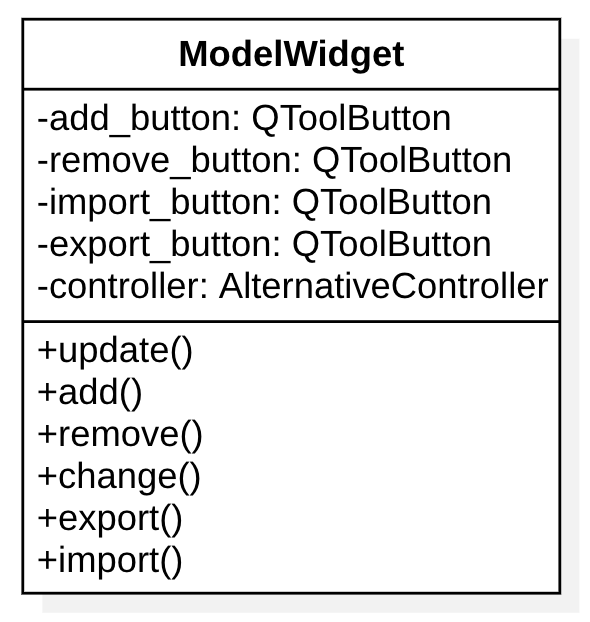
\includegraphics[width=5cm]{entwurf/Entwurf_dokument/img/klassenView/ModelWidget.png}
        \caption{Die Klasse ModelWidget}
    \end{minipage}
    \hfill
    \begin{minipage}[b]{0.4\textwidth}
        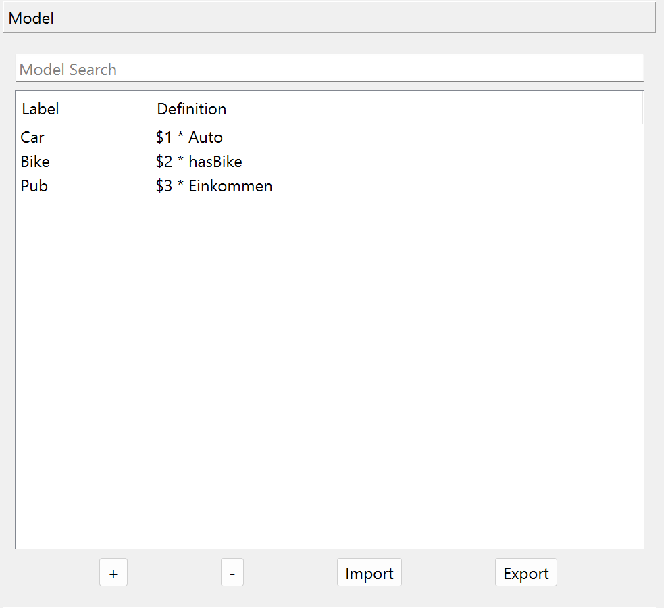
\includegraphics[width=5cm]{entwurf/Entwurf_dokument/img/Alissa/ModelGUI.png} 
    \caption{Das \textit{Model} Fenster in der GUI.}
    \end{minipage}
\end{figure}
Die Klasse \textit{ModelWidget} repräsentiert die Tabelle im Hauptfenster, die die Alternativen darstellt.
\newline

\textbf{{Attribute}}
\begin{itemize}
\item \texttt{add\char`_button: QToolButton} \newline Diese Schaltfläche erlaubt dem Nutzer, eine neue Alternative zu definieren.
\item \texttt{remove\char`_button: QToolButton} \newline Mit dieser Schaltfläche kann der Nutzer eine bestehende Alternative löschen
\item \texttt{import\char`_char: QToolButton} \newline Ermöglicht dem Nutzer Alternativen zu importieren.
\item \texttt{export\char`_button: QToolButton} \newline Ermöglicht dem Nutzer Alternativen zu exportieren.
\item \texttt{controller: AlternativeController} \newline Der Controller, der die Nutzeranfragen bzgl. der Alternativen im Model verarbeitet.
\end{itemize}

\textbf{{Methoden}}
\begin{itemize}
\item \texttt{update()} \newline Aktualisiert die dem Nutzer angezeigten Informationen. Nach der Ausführung einer der Verwaltungsoperationen an den Alternativen wird duch diese Funktion die Ansicht aktualisiert. Das Widget benachrichtigt den Controller, und dieser holt die notwendigen Informationen zur Abbildung aus dem Model.

\item \texttt{add()} \newline Fügt eine neue Alternative hinzu. Dazu werden dem Nutzer Textfelder erstellt, in die sowohl Name als auch Nutzenfunktion einer Alternative eingegeben werden sollen.

\item \texttt{remove()} \newline Löscht die ausgewählte Alternative aus dem Model. Ist keine ausgewählt passiert nichts beim Betätigen dieses Buttons.

\item \texttt{change()} \newline Ändert eine schon eingegebene Alternative. Der Nutzer ändert eine Alternative in der Darstellung und diese Methode leitet die Informationen an den Controller weiter, welcher diese im Model umsetzen lässt.

\item \texttt{export()} \newline Exportiert die Alternativen zu einem nutzerdefiniertem Speicherort. 

\item \texttt{import()} \newline Importiert Alternativen aus einer CSV oder JSON Datei.
\end{itemize}

\newpage
\subsection{Model}
\subsubsection{Data}
\classheader[\flqq{}immutable\frqq]{Model}\label{cls:Model}
\begin{tabular}{lll}
 Superklassen: & --\\
 Subklassen: & --\\
\end{tabular}\\
\begin{figure}[H]%
    \centering
    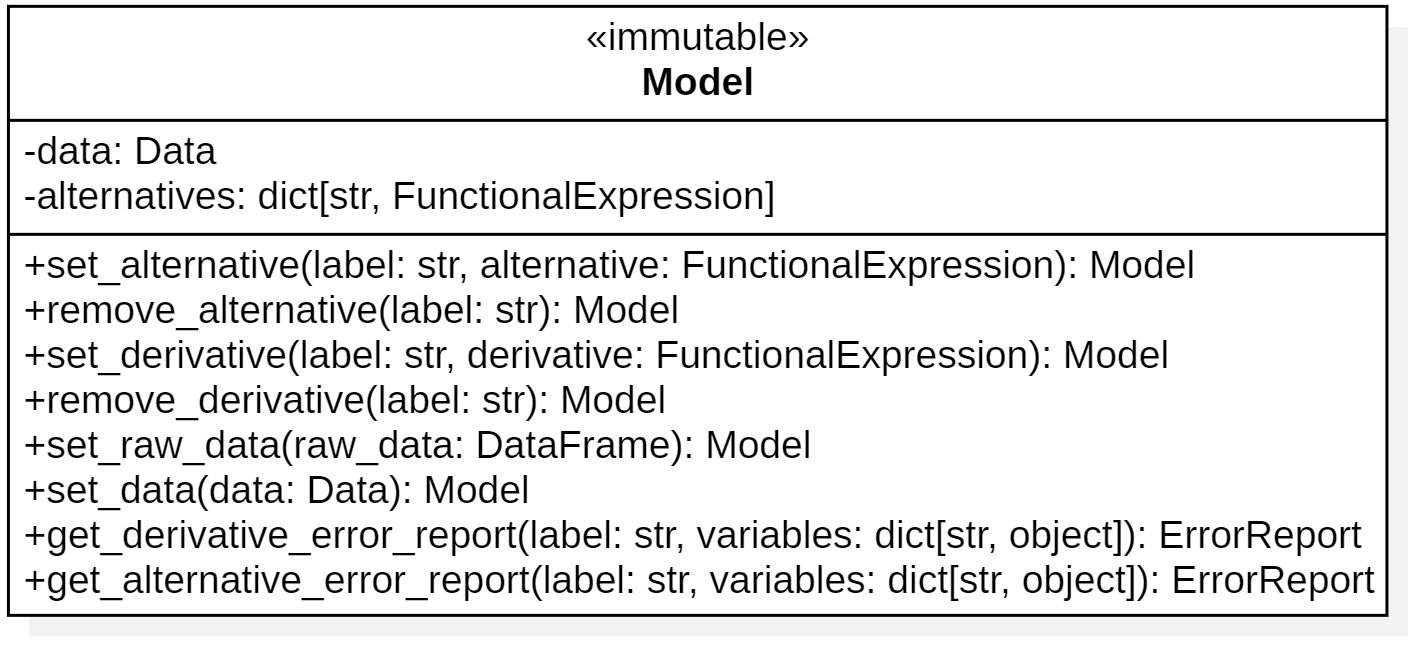
\includegraphics[width=13cm]{entwurf/Entwurf_dokument/img/cls/model/Model.png}
    \caption{Klassendiagramm \texttt{Model}}
\end{figure}

Verwaltet die Daten, die das Modell definieren und wird als Eingabe der Berechnung verwendet. Die Klasse ist die Schnittstelle bei Abfragen und Änderungen des Modells.\\
Die Klasse nimmt Bezug auf \texttt{DataFrame} aus dem externen Paket \texttt{pandas} um die importierten Rohdaten des Nutzers zu speichern.
\newline \newline

\textbf{{Attribute}}
\begin{itemize}
\item \texttt{data: Data} \newline In das Projekt importierte Erhebungsdaten und Schnittstelle zur Verwaltung der Ableitungen.
\item \texttt{alternatives: dict[label: str, expr: FunctionalExpression]} \newline
Definierte Alternativen mit eindeutigem Bezeichner.
\\\\
\end{itemize}

\textbf{{Methoden}}
\begin{itemize}
\item \texttt{set\char`_alternative(label: str, alternative: FunctionalExpression): Model} \newline Hinzufügen oder Ändern einer Alternative. Das \texttt{Model}-Objekt wird dabei nicht verändert, sondern gibt eine Kopie mit der Veränderung zurück.
\\\\
\underline{{Parameter}}

\begin{tabular}{lll}
 & \texttt{label} & Eindeutiger Bezeichner der Alternative. \\
 & \texttt{alternative} & Funktionaler Ausdruck der Alternative. \\
\end{tabular}

\underline{{Rückgabewert}}

\begin{tabular}{lll}
 & \texttt{Model} & \texttt{Model} nach Veränderung der Alternative. \\
\end{tabular}

\underline{Exceptions}\\
\begin{tabular}{lll}
 & \texttt{ValueError} & Bezeichner der Alternative ist ungültig.\\
\end{tabular}


\item \texttt{remove\char`_alternative(label: str): Model} \newline Entfernen einer existierenden Alternative. \texttt{Model} wird dabei nicht verändert, sondern gibt eine Kopie mit der Veränderung zurück.
\\\\
\underline{{Parameter}}

\begin{tabular}{lll}
 & \texttt{label} & Eindeutiger Bezeichner der Alternative. \\
\end{tabular}

\underline{{Rückgabewert}}

\begin{tabular}{lll}
 & \texttt{Model} & \texttt{Model} nach Entfernen der Alternative. \\
\end{tabular}

\underline{Exceptions}\\
\begin{tabular}{lll}
 & \texttt{ValueError} & Bezeichner der Alternative existiert nicht.\\
\end{tabular}


\item \texttt{set\char`_derivative(label: str, derivative: FunctionalExpression): Model} \newline Hinzufügen oder Ändern einer Ableitung im assoziierten \texttt{Data}-Objekt. Das \texttt{Model}-Objekt wird dabei nicht verändert, sondern gibt eine Kopie mit der Veränderung zurück.
\\\\
\underline{{Parameter}}

\begin{tabular}{lll}
 & \texttt{label} & Eindeutiger Bezeichner der Ableitung. \\
 & \texttt{derivative} & Ausdruck der Ableitung. \\
\end{tabular}

\underline{{Rückgabewert}}

\begin{tabular}{lll}
 & \texttt{Model} & \texttt{Model} nach Veränderung der Ableitung. \\
\end{tabular}

\underline{Exceptions}\\
\begin{tabular}{lll}
 & \texttt{ValueError} & Ableitungsbezeichner ist ungültig.\\
\end{tabular}


\item \texttt{remove\char`_derivative(label: str): Model} \newline Entfernen einer existierenden Ableitung im assoziierten \texttt{Data}-Objekt. Das \texttt{Model}-Objekt wird dabei nicht verändert, sondern gibt eine Kopie mit der Veränderung zurück.
\\\\
\underline{{Parameter}}

\begin{tabular}{lll}
 & \texttt{label} & Eindeutiger Bezeichner der Ableitung. \\
\end{tabular}

\underline{{Rückgabewert}}

\begin{tabular}{lll}
 & \texttt{Model} & \texttt{Model} nach Entfernen der Ableitung. \\
\end{tabular}

\underline{Exceptions}\\
\begin{tabular}{lll}
 & \texttt{ValueError} & Ableitungsbezeichner existiert nicht.\\
\end{tabular}


\item \texttt{set\char`_raw\char`_data(raw\char`_data: DataFrame): Model} \newline Verändern der Erhebungsdaten im assoziierten \texttt{Data}-Objekt. Das \texttt{Model}-Objekt wird dabei nicht verändert, sondern gibt eine Kopie mit der Veränderung zurück.
\\\\
\underline{{Parameter}}

\begin{tabular}{lll}
 & \texttt{raw\char`_data} & Importierte Rohdaten für das Modell. \\
\end{tabular}

\underline{{Rückgabewert}}

\begin{tabular}{lll}
 & \texttt{Model} & \texttt{Model} nach Veränderung der Rohdaten. \\
\end{tabular}


\item \texttt{set\char`_data(data: Data): Model} \newline Verändern der Erhebungsdaten oder der Ableitungen. Das \texttt{Model}-Objekt wird dabei nicht verändert, sondern gibt eine Kopie mit der Veränderung zurück.
\\\\
\underline{{Parameter}}

\begin{tabular}{lll}
 & \texttt{data} & Neues \texttt{Data}-Objekt mit angewandter Veränderung. \\
\end{tabular}

\underline{{Rückgabewert}}

\begin{tabular}{lll}
 & \texttt{Model} & \texttt{Model} nach Veränderung des \texttt{Data}-Objekts. \\
\end{tabular}


\item \texttt{get\char`_derivative\char`_error\char`_report(label: str, variables: dict[str, object]): ErrorReport} \newline Identifizieren aller Fehler in dem Ausdruck der Ableitung. Anhand des \texttt{ErrorReport}-Objekts in der Rückgabe können die Fehlermeldungen zusätzlich visualisiert werden.
\\\\
\underline{{Parameter}}

\begin{tabular}{lll}
 & \texttt{label} & Eindeutiger Bezeichner der Ableitung. \\
 & \texttt{variables} & Vorhandene und in einer Ableitung verwendbare Variablen. \\&& Verwendet zur Identifizierung von Typ- und Referenzfehlern. \\
\end{tabular}

\underline{{Rückgabewert}}

\begin{tabular}{lll}
 & \texttt{ErrorReport} & Kollektion aller Fehlermeldungen in der Ableitung. \\
\end{tabular}

\underline{Exceptions}\\
\begin{tabular}{lll}
 & \texttt{ValueError} & Ableitungsbezeichner existiert nicht.\\
\end{tabular}


\item \texttt{get\char`_alternative\char`_error\char`_report(label: str, variables: dict[str, object]): ErrorReport} \newline Identifizieren aller Fehler in der referenzierten Alternative. Anhand des \texttt{ErrorReport}-Objekts in der Rückgabe können die Fehlermeldungen zusätzlich visualisiert werden.
\\\\
\underline{{Parameter}}

\begin{tabular}{lll}
 & \texttt{label} & Eindeutiger Bezeichner der Alternative. \\
 & \texttt{variables} & Vorhandene und in einer Alternative verwendbare Variablen. \\&& Verwendet zur Identifizierung von Typ- und Referenzfehlern. \\
\end{tabular}

\underline{{Rückgabewert}}

\begin{tabular}{lll}
 & \texttt{ErrorReport} & Kollektion aller Fehlermeldungen in der Alternative. \\
\end{tabular}

\underline{Exceptions}\\
\begin{tabular}{lll}
 & \texttt{ValueError} & Bezeichner der Alternative existiert nicht.\\
\end{tabular}
\end{itemize}

\newpage
\classheader[\flqq{}immutable\frqq]{Data}\label{cls:Data}
\begin{tabular}{lll}
 Superklassen: & --\\
 Subklassen: & --\\
\end{tabular}\\
\begin{figure}[H]%
    \centering
    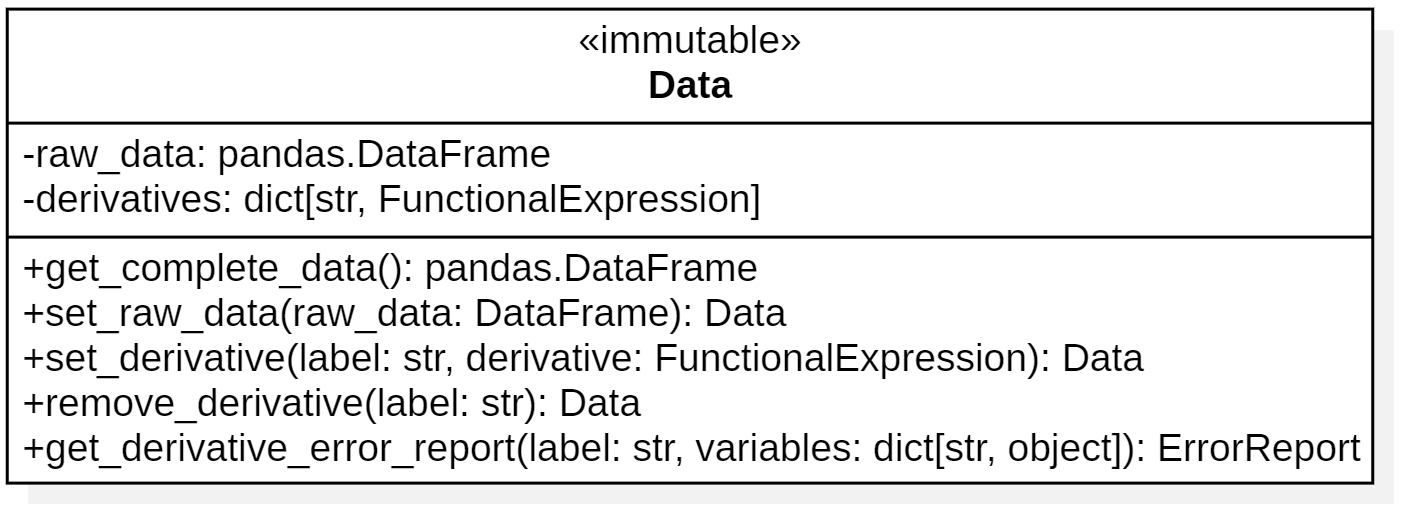
\includegraphics[width=13cm]{entwurf/Entwurf_dokument/img/cls/model/Data.png}
    \caption{Klassendiagramm \texttt{Data}}
\end{figure}

Verwaltet die Daten der importierten Erhebungsdaten und der Ableitungen. Abfragen und Änderungen werden über die Klasse \classref{Model} aufgerufen.\\
Die Klasse nimmt Bezug auf \texttt{DataFrame} aus dem externen Paket \texttt{pandas} um die importierten Rohdaten des Nutzers zu speichern.
\newline \newline

\textbf{{Attribute}}
\begin{itemize}
\item \texttt{raw\char`_data: DataFrame} \newline Importierte Rohdaten.
\item \texttt{derivatives: dict[label: str, expr: FunctionalExpression]} \newline Definierte Ableitungen mit eindeutigem Bezeichner.
\\\\
\end{itemize}

\textbf{{Methoden}}
\begin{itemize}
\item \texttt{get\char`_complete\char`_data(): DataFrame} \newline Erzeugt ein neues \texttt{DataFrame}, das die Rohdaten und die berechneten Ableitungen zusammensetzt.
\\\\
\underline{{Rückgabewert}}

\begin{tabular}{lll}
 & \texttt{DataFrame} & Zusammensetzung der Rohdaten mit den berechneten Ableitungen. \\
\end{tabular}

\item \texttt{set\char`_raw\char`_data(raw\char`_data: DataFrame): Data} \newline Verändern der Rohdaten. \texttt{Data} wird dabei nicht verändert, sondern gibt eine Kopie mit der Veränderung zurück.
\\\\
\underline{{Parameter}}

\begin{tabular}{lll} 
 & \texttt{raw\char`_data} & Importierte Rohdaten für das Modell. \\
\end{tabular}

\underline{{Rückgabewert}}

\begin{tabular}{lll}
 & \texttt{Data} & \texttt{Data} nach Veränderung der Rohdaten.  \\
\end{tabular}

\item \texttt{set\char`_derivative(label: str, derivative: FunctionalExpression): Data} \newline Hinzufügen oder Ändern einer Ableitung. Das \texttt{Data}-Objekt wird dabei nicht verändert, sondern gibt eine Kopie mit der Veränderung zurück.
\\\\
\underline{{Parameter}}

\begin{tabular}{lll}
 & \texttt{label} & Eindeutiger Bezeichner der Ableitung. \\
 & \texttt{derivative} & Ausdruck der Ableitung. \\
\end{tabular}

\underline{{Rückgabewert}}

\begin{tabular}{lll}
 & \texttt{Data} & \texttt{Data} nach Veränderung der Ableitung. \\
\end{tabular}

\underline{Exceptions}\\
\begin{tabular}{lll}
 & \texttt{ValueError} & Ableitungsbezeichner ist ungültig.\\
\end{tabular}


\item \texttt{remove\char`_derivative(label: str): Data} \newline Entfernen einer existierenden Ableitung. Das \texttt{Data}-Objekt wird dabei nicht verändert, sondern gibt eine Kopie mit der Veränderung zurück.
\\\\
\underline{{Parameter}}

\begin{tabular}{lll}
 & \texttt{label} & Eindeutiger Bezeichner der Ableitung. \\
\end{tabular}

\underline{{Rückgabewert}}

\begin{tabular}{lll}
 & \texttt{Data} & \texttt{Data} nach Entfernen der Ableitung. \\
\end{tabular}

\underline{Exceptions}\\
\begin{tabular}{lll}
 & \texttt{ValueError} & Ableitungsbezeichner existiert nicht.\\
\end{tabular}

\item \texttt{get\char`_derivative\char`_error\char`_report(label: str, variables: dict[str, object]): ErrorReport} \newline Identifizieren aller Fehler in dem Ausdruck der Ableitung. Anhand des \texttt{ErrorReport}-Objekts in der Rückgabe können die Fehlermeldungen zusätzlich visualisiert werden.
\\\\
\underline{{Parameter}}

\begin{tabular}{lll}
 & \texttt{label} & Eindeutiger Bezeichner der Ableitung. \\
 & \texttt{variables} & Vorhandene und in einer Ableitung verwendbare Variablen. \\&& Verwendet zur Identifizierung von Typ- und Referenzfehlern. \\
\end{tabular}

\underline{{Rückgabewert}}

\begin{tabular}{lll}
 & \texttt{ErrorReport} & Kollektion aller Fehlermeldungen in der Ableitung. \\
\end{tabular}

\underline{Exceptions}\\
\begin{tabular}{lll}
 & \texttt{ValueError} & Ableitungsbezeichner existiert nicht.\\
\end{tabular}
\end{itemize}

\newpage
\subsubsection{Functions}
\classheader[\flqq{}immutable\frqq]{FunctionalExpression}\label{cls:FunctionalExpression}
\begin{tabular}{lll}
 Superklassen: & --\\
 Subklassen: & --\\
\end{tabular}\\
\begin{figure}[H]%
    \centering
    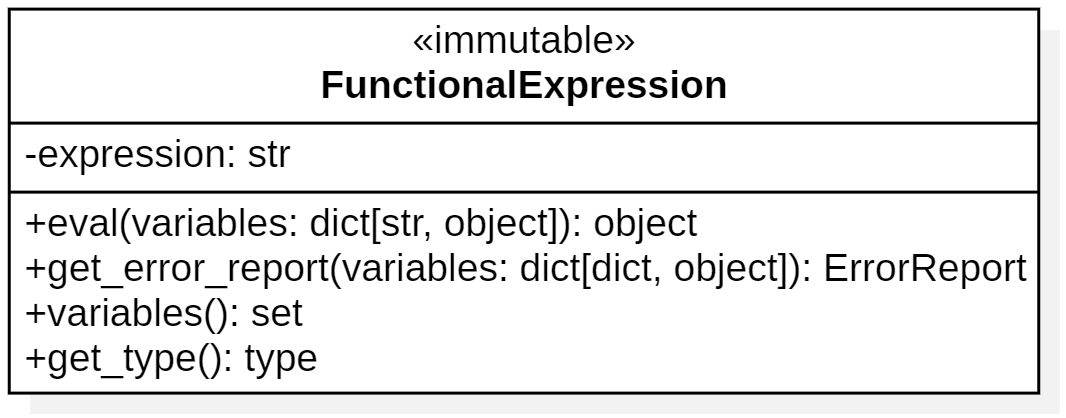
\includegraphics[width=10cm]{entwurf/Entwurf_dokument/img/cls/model/FunctionalExpression.png}
    \caption{Klassendiagramm \texttt{FunctionalExpression}}
\end{figure}

Repräsentation des Funktionsausdrucks einer definierten Attributsableitung oder Alternative.
\newline \newline

\textbf{{Attribute}}
\begin{itemize}
\item \texttt{expression: str} \newline Funktionsausdruck in textueller Form.
\\\\
\end{itemize}

\textbf{{Methoden}}
\begin{itemize}
\item \texttt{eval(variables: dict[str, object])} \newline Evaluiert den gespeicherten Funktionsausdruck.
\\\\
\underline{{Parameter}}

\begin{tabular}{lll}
 & \texttt{variables} & Feste Zuweisungen der Variablen zu den damit definierten Objekten. \\&& Diese Variablen können im Ausdruck verwendet werden. \\
\end{tabular}

\underline{{Rückgabewert}}

\begin{tabular}{lll}
 & \texttt{object} & Berechnetes Ergebnis nach Evaluierung des Ausdrucks. \\
\end{tabular}

\item \texttt{get\char`_error\char`_report(variables: dict[dict, object]): ErrorReport} \newline Erstellt eine Sammlung aller identifizierten Fehler in dem funktionalen Ausdruck. Dieser \texttt{ErrorReport} wird verwendet.
\\\\
\underline{{Parameter}}

\begin{tabular}{lll}
 & \texttt{variables} & Feste Zuweisungen der Variablen zu den damit definierten Objekten. \\&& Diese Variablen können im Ausdruck verwendet werden. \\
\end{tabular}

\underline{{Rückgabewert}}

\begin{tabular}{lll}
 & \texttt{ErrorReport} & \texttt{True}, wenn der Ausdruck syntaktisch korrekt ist. \\&& Andernfalls \texttt{False}. \\
\end{tabular}

\item \texttt{variables(): set} \newline Gibt die im Ausdruck verwendeten Variablen zurück.
\\\\
\underline{{Rückgabewert}}

\begin{tabular}{lll}
 & \texttt{set} & Verwendete Variablen im Ausdruck. \\
\end{tabular}

\item \texttt{get\char`_type(): type} \newline Gibt den resultierenden Datentypen nach Evaluierung des Ausdrucks zurück.
\\\\
\underline{{Rückgabewert}}

\begin{tabular}{lll}
 & \texttt{type} & Datentyp des Ausdrucks. \\
\end{tabular}
\end{itemize}


\newpage
\classheader[\flqq{}immutable\frqq]{Interval}\label{cls:Interval}
\begin{tabular}{lll}
 Superklassen: & --\\
 Subklassen: & --\\
\end{tabular}\\
\begin{figure}[H]%
    \centering
    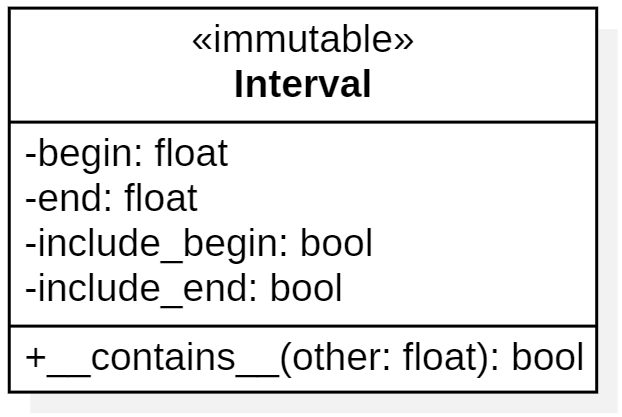
\includegraphics[width=6cm]{entwurf/Entwurf_dokument/img/cls/model/Interval.png}
    \caption{Klassendiagramm \texttt{Interval}}
\end{figure}

Darstellung eines Intervalls. Definierbar bei Festlegung der Ableitungen (siehe \classref{FunctionalExpression}). Wird bei der Evaluation der Ableitung erzeugt und kann ausgewertet werden.
\newline \newline

\textbf{{Attribute}}
\begin{itemize}
\item \texttt{begin: float} \newline Beginn des Intervalls. \texttt{None} bei fehlender unterer Intervallgrenze. 
\item \texttt{end: float} \newline Ende des Intervalls. \texttt{None} bei fehlender oberer Intervallgrenze. 
\item \texttt{include\char`_begin: bool} \newline Intervall inkludiert den Beginn.
\item \texttt{include\char`_end: bool} \newline Intervall inkludiert das Ende.
\\\\
\end{itemize}

\textbf{{Methoden}}
\begin{itemize}
\item \texttt{\char`_\char`_contains\char`_\char`_(other: float): bool} \newline Überprüft ob ein Wert im Intervall liegt.
\\\\
\underline{{Parameter}}

\begin{tabular}{lll}
 & \texttt{other} & Zu überprüfender Wert. \\
\end{tabular}

\underline{{Rückgabewert}}

\begin{tabular}{lll}
 & \texttt{bool} & \texttt{True}, falls der Wert im Intervall liegt. Andernfalls \texttt{False}. \\
\end{tabular}
\end{itemize}


\newpage
\classheader[\flqq{}immutable\frqq]{GroupMap}\label{cls:GroupMap}
\begin{tabular}{lll}
 Superklassen: & --\\
 Subklassen: & --\\
\end{tabular}\\
\begin{figure}[H]%
    \centering
    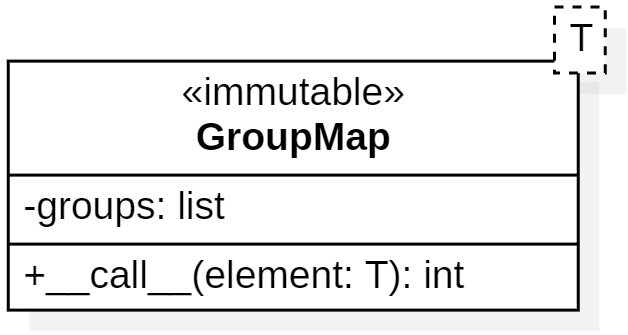
\includegraphics[width=7cm]{entwurf/Entwurf_dokument/img/cls/model/GroupMap.png}
    \caption{Klassendiagramm \texttt{GroupMap}}
\end{figure}

Darstellung einer Liste von Gruppen mit Elementen. Definierbar bei Festlegung der Ableitungen (siehe \classref{FunctionalExpression}). Wird bei der Evaluation der Ableitung erzeugt und kann ausgewertet werden.
\newline \newline

\textbf{Attribute}
\begin{itemize}
\item \texttt{groups: list} \newline Liste der Gruppen mit Elementen.
\\\\
\end{itemize}

\textbf{Methoden}
\begin{itemize}
\item \texttt{\char`_\char`_call\char`_\char`_(element: T): int} \newline Überprüft in welcher Gruppe sich ein Element befindet und gibt den Index zurück.
\\\\
\underline{{Parameter}}

\begin{tabular}{lll}
 & \texttt{element} & Zu überprüfendes Element. \\
\end{tabular}

\underline{Rückgabewert}

\begin{tabular}{lll}
 & \texttt{int} & Index der Gruppe, in welcher sich das Element befindet. \\
 && \texttt{None}, falls in keiner der Gruppen.\\
\end{tabular}
\end{itemize}


\newpage
\classheader[\flqq{}immutable\frqq]{ErrorReport}\label{cls:ErrorReport}
\begin{tabular}{lll}
 Superklassen: & --\\
 Subklassen: & --\\
\end{tabular}\\
\begin{figure}[H]%
    \centering
    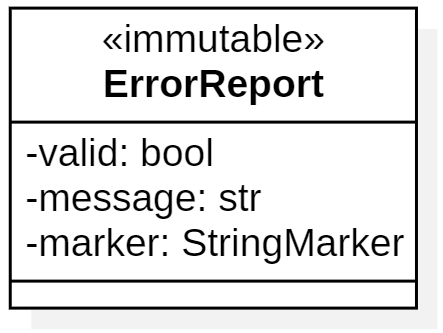
\includegraphics[width=7cm]{entwurf/Entwurf_dokument/img/cls/model/ErrorReport.png}
    \caption{Klassendiagramm \texttt{ErrorReport}}
\end{figure}

Beschreibt Fehlermeldungen in Ausdrücken der \classref{FunctionalExpression}-Klasse. \\ Ermöglicht eine visuelle Repräsentation der Fehlermeldung am invaliden Ausdruck.
\newline \newline

\textbf{Attribute}
\begin{itemize}
\item \texttt{valid: bool} \newline Wird bei Erstellung des Objekts erstellt. Ist \texttt{True}, wenn die \texttt{FunctionalExpression} keine Fehler besitzt. Andernfalls \texttt{False}.
\item \texttt{marker: list[StringMarker]} \newline Visualisierbare Position eines Fehlers mit Fehlernachricht.
\\\\
\end{itemize}


\newpage
\classheader[\flqq{}immutable\frqq]{StringMarker}\label{cls:StringMarker}
\begin{tabular}{lll}
 Superklassen: & --\\
 Subklassen: & --\\
\end{tabular}\\
\begin{figure}[H]%
    \centering
    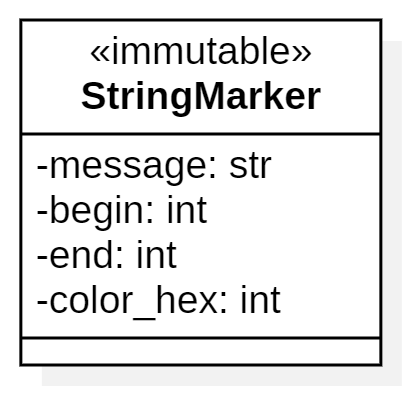
\includegraphics[width=5cm]{entwurf/Entwurf_dokument/img/cls/model/StringMarker.png}
    \caption{Klassendiagramm \texttt{StringMarker}}
\end{figure}

Speichert die Markierung eines Substrings und eine Nachricht. Wird bei Ferhlermeldung zu einer \classref{FunctionalExpression} verwendet, um einen Fehler eindeutig zu visualisieren.
\newline \newline

\textbf{Attribute}
\begin{itemize}
\item \texttt{message: str} \newline Textuelle Beschreibung des Fehlers.
\item \texttt{begin: int} \newline Beginn des Substrings, auf den sich die Fehlermeldung bezieht.
\item \texttt{end: int} \newline Ende des Substrings, auf den sich die Fehlermeldung bezieht.
\item \texttt{color\char`_hex: int} \newline Farbe der Hervorhebung als RGB kodiert in Hexadezimal.
\\\\
\end{itemize}


\newpage
\subsubsection{Processing}

%----------------------------------
\classheader[\flqq{}abstract\frqq \mbox{} \flqq{}immutable\frqq]{ProcessingConfig}\label{cls:ProcessingConfig}
\begin{tabular}{lll}
 Superklassen: & --\\
 Subklassen: & \texttt{SimpleProcessingConfig}, \texttt{VariedProcessingConfig}
\end{tabular}\\
\begin{figure}[H]%
    \centering
    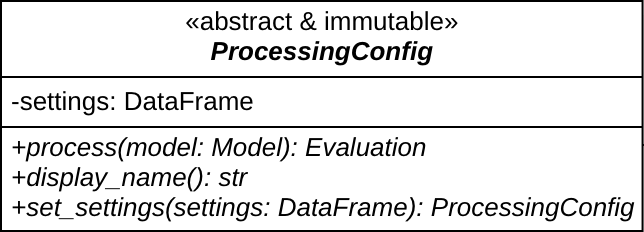
\includegraphics[width=13cm]{entwurf/Entwurf_dokument/img/cls/model/ProcessingConfig.png}
    \caption{Klassendiagramm \texttt{ProcessingConfig}}
\end{figure}

Die Klasse definiert, auf welche Art und Weise eine Datenverarbeitung eines Datenmodells erfolgt.
\\\\

\textbf{Attribute}
\begin{itemize}\setlength\itemsep{3em}
\item \texttt{settings: pandas.DataFrame}\\\\
Datentabelle der Nutzereinstellungen.
\\\\
\end{itemize}

\textbf{Methoden}
\begin{itemize}\setlength\itemsep{3em}
\item \textit{\flqq{}abstract\frqq} \texttt{\textit{process(model: Model): Evaluation}}\\\\
Verarbeitet ein \texttt{model} entsprechend der Konfigurationsklasse und erstellt eine Auswertung vom Typ \texttt{Evaluation}.
\\\\
\underline{Parameter}\\
\begin{tabular}{lll}
 & \texttt{model} & Diskretes Wahlmodell, auf dem eine Verabreitung erfolgen soll.\\
\end{tabular}

\underline{Rückgabewert}\\
\begin{tabular}{lll}
 & Auswertung, wie durch Konfigurationsklasse definiert.\\
\end{tabular}

\underline{Exceptions}\\
\begin{tabular}{lll}
 & \texttt{ValueError} & Modell hat nicht die durch die Konfiguration geforderten Eigenschaften.\\
\end{tabular}

\item \textit{\flqq{}abstract\frqq} \texttt{\textit{display\char`_name(): str}}\\\\
Getter für Anzeigename der Konfigurationsklasse zur Darstellung im Auswahlmenü.
\\\\
\underline{Rückgabewert}\\
\begin{tabular}{lll}
 & Anzeigename als \texttt{str}.\\
\end{tabular}

\item \textit{\flqq{}abstract\frqq} \texttt{\textit{set\char`_settings(settings: pandas.DataFrame): ProcessingConfig}}\\\\
Erstellt eine Kopie des Objekts, in der lediglich das Attribut \texttt{settings} durch das übergebene Attribut überschrieben wird.
\\\\
\underline{Parameter}\\
\begin{tabular}{lll}
 & \texttt{settings} & Neue Datentabelle der Nutzereinstellungen.\\
\end{tabular}

\underline{Rückgabewert}\\
\begin{tabular}{lll}
 & Anzeigename als \texttt{str}.\\
\end{tabular}
\end{itemize}

%----------------------------------
\newpage
\classheader[\flqq{}immutable\frqq]{SimpleProcessingConfig}\label{cls:SimpleProcessingConfig}
\begin{tabular}{lll}
 Superklassen: & \texttt{ProcessingConfig}\\
 Subklassen: & --
\end{tabular}\\
\begin{figure}[H]%
    \centering
    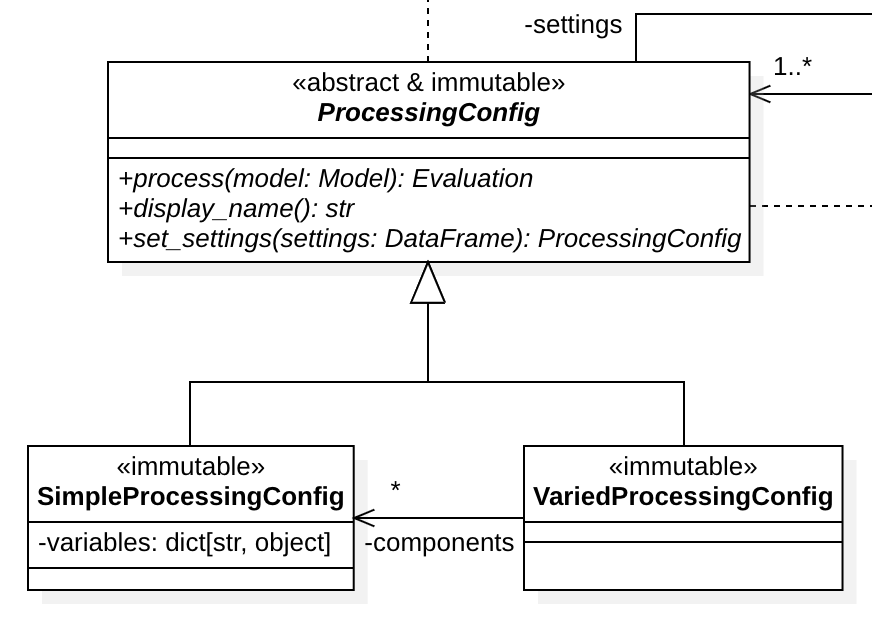
\includegraphics[width=13cm]{entwurf/Entwurf_dokument/img/cls/model/ProcessingConfigs.png}
    \caption{Klassendiagramm aller Subklassen von \texttt{ProcessingConfig}}
\end{figure}

Die Klasse definiert das Verfahren einer einfachen Parameterschätzung eines diskreten Wahlmodells und weist den verbleibenden freie Variablen im Modell einen Wert zu.
\\\\

\textbf{Attribute}
\begin{itemize}\setlength\itemsep{3em}
\item \texttt{variables: dict[str, object]}\\\\
Zuordnung zwischen verbleibenden freien Variablen und einem Wert, der für die Berechnung verwendet werden soll.\\
Der Datentyp der Werte kann nicht weiter eingeschränkt werden, da dieser von der Verwendung der freien Variablen abhängt.
\\\\
\end{itemize}

\textbf{Methoden}
\begin{itemize}\setlength\itemsep{3em}
\item \texttt{process(model: Model): Evaluation}\\\\
Wendet die definierte Parameterschätzung auf \texttt{model} an und erstellt eine Auswertung vom Typ \texttt{Evaluation}.
\\\\
\underline{Parameter}\\
\begin{tabular}{lll}
 & \texttt{model} & Diskretes Wahlmodell, auf dem eine Verarbeitung erfolgen soll.\\
\end{tabular}

\underline{Rückgabewert}\\
\begin{tabular}{lll}
 & Auswertung, wie durch Konfigurationsklasse definiert.\\
\end{tabular}

\underline{Exceptions}\\
\begin{tabular}{lll}
 & \texttt{ValueError} & Modell hat nicht die durch die Konfiguration geforderten Eigenschaften.\\
\end{tabular}
\end{itemize}

%----------------------------------
\newpage
\classheader[\flqq{}immutable\frqq]{VariedProcessingConfig}\label{cls:VariedProcessingConfig}
\begin{tabular}{lll}
 Superklassen: & \texttt{ProcessingConfig}\\
 Subklassen: & --
\end{tabular}\\
\begin{figure}[H]%
    \centering
    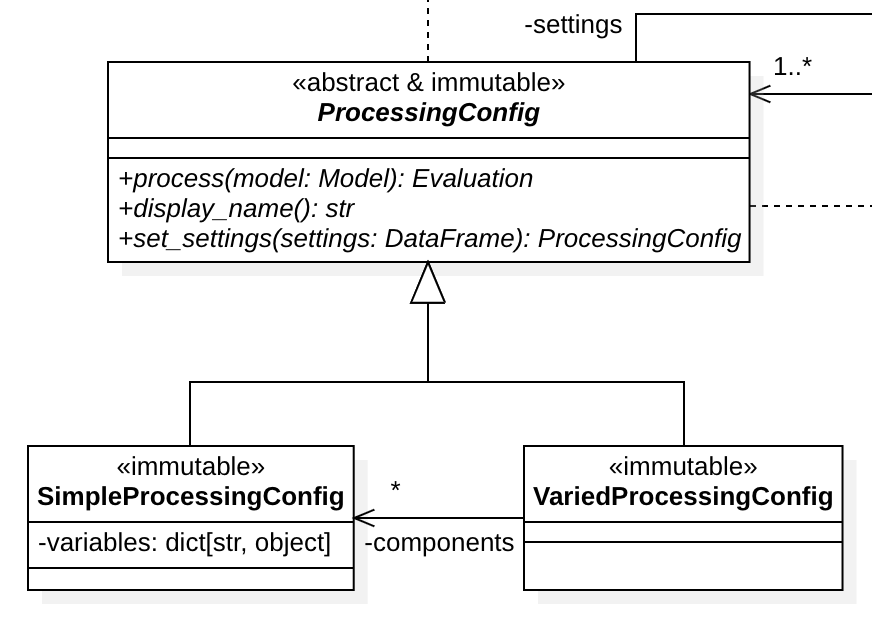
\includegraphics[width=13cm]{entwurf/Entwurf_dokument/img/cls/model/ProcessingConfigs.png}
    \caption{Klassendiagramm aller Subklassen von \texttt{ProcessingConfig}}
\end{figure}

Die Klasse definiert eine mehrfache Anwendung einer Parameterschätzung eines diskreten Wahlmodells und weist dabei den verbleibenden freie Variablen im Modell je unterschiedliche Werte zu. Die Werte können definiert werden und müssen vor dem Aufruf von \texttt{process} vorliegen.
\\\\

\textbf{Attribute}
\begin{itemize}\setlength\itemsep{3em}
\item \texttt{components: list[SimpleProcessingConfig]}\\\\
Liste von Konfigurationen vom Typ \texttt{SimpleProcessingConfig}, die nacheinander ausgeführt werden sollen.
\\\\
\end{itemize}

\textbf{Methoden}
\begin{itemize}\setlength\itemsep{3em}
\item \texttt{process(model: Model): Evaluation}\\\\
Wendet alle hinterlegten einzelnen Parameterschätzungen auf \texttt{model} an und erstellt eine Auswertung vom Typ \texttt{Evaluation}.
\\\\
\underline{Parameter}\\
\begin{tabular}{lll}
 & \texttt{model} & Diskretes Wahlmodell, auf dem eine Verabreitung erfolgen soll.\\
\end{tabular}

\underline{Rückgabewert}\\
\begin{tabular}{lll}
 & Auswertung, wie durch Konfigurationsklasse definiert.\\
\end{tabular}

\underline{Exceptions}\\
\begin{tabular}{lll}
 & \texttt{ValueError} & Modell hat nicht die durch die Konfiguration geforderten Eigenschaften.\\
\end{tabular}
\end{itemize}

%----------------------------------
\newpage
\classheader[\flqq{}immutable\frqq]{Evaluation}\label{cls:Evaluation}
\begin{tabular}{lll}
 Superklassen: & --\\
 Subklassen: & --
\end{tabular}\\
\begin{figure}[H]%
    \centering
    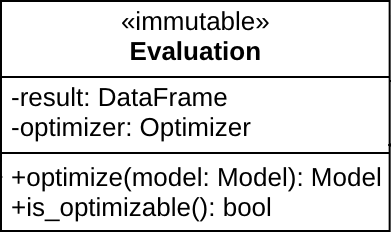
\includegraphics[width=13cm]{entwurf/Entwurf_dokument/img/cls/model/Evaluation.png}
    \caption{Klassendiagramm von \texttt{Evaluation}}
\end{figure}

Die Klasse entspricht der Auswertung einer Parameterschätzung von einem diskreten Wahlmodell.
\\\\

\textbf{Attribute}
\begin{itemize}\setlength\itemsep{3em}
\item \texttt{result: pandas.DataFrame}\\\\
Auswertungstabelle der verwendeten Berechnungsbibliothek oder eine zusammengesetzte Tabelle aus mehreren Auswertungstabellen.
\\\\
\end{itemize}

\textbf{Methoden}
\begin{itemize}\setlength\itemsep{3em}
\item \texttt{optimize(model: Model): Model}\\\\
Falls der Auswertung ein Modelloptimierungsverfahren beiliegt (siehe \texttt{is\char`_optimizable()}), wird das diskrete Wahlmodell dementsprechend verbessert.\\\\
\underline{Parameter}\\
\begin{tabular}{lll}
 & \texttt{model} & Diskretes Wahlmodell, das optimiert werden soll.\\
\end{tabular}

\underline{Rückgabewert}\\
\begin{tabular}{lll}
 & Das optimierte diskrete Wahlmodell.\\
\end{tabular}

\underline{Exceptions}\\
\begin{tabular}{lll}
 & \texttt{ValueError} & Modell hat nicht die durch den Optimierungsalgorithmus\\
 && geforderten Eigenschaften.\\
\end{tabular}

\item \texttt{is\char`_optimizable(): bool}\\\\
Prüft, ob eine Optimierung auf Grundlage dieser Auswertung prinzipiell möglich ist.\\\\
\underline{Parameter}\\
\begin{tabular}{lll}
 & Keine Parameter.
\end{tabular}

\underline{Rückgabewert}\\
\begin{tabular}{lll}
 & Wahrheitswert, ob Optimierung auf Grundlage dieser Auswertung prinzipiell möglich ist.\\
\end{tabular}
\end{itemize}


%----------------------------------
\newpage
\classheader[\flqq{}interface\frqq]{Optimizer}\label{cls:Optimizer}
\begin{tabular}{lll}
 Superklassen: & --\\
 Subklassen: & --
\end{tabular}\\
\begin{figure}[H]%
    \centering
    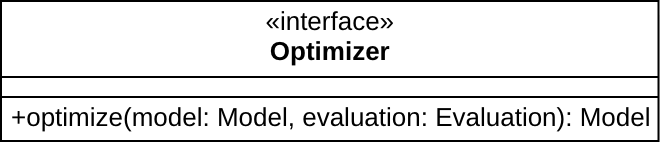
\includegraphics[width=13cm]{entwurf/Entwurf_dokument/img/cls/model/Optimizer.png}
    \caption{Klassendiagramm von \texttt{Optimizer}}
\end{figure}

Das Interface bietet eine Schnittstelle zur Implementierung eines beliebigen Optimierungsalgorithmus.
\\\\

\textbf{Methoden}
\begin{itemize}\setlength\itemsep{3em}
\item \textit{\flqq{}abstract\frqq} \texttt{\textit{optimize(model: Model, evaluation: Evaluation): Model}}\\\\
Falls der Auswertung ein Modelloptimierungsverfahren beiliegt (siehe \texttt{is\char`_optimizable()}), wird das diskrete Wahlmodell dementsprechend verbessert.\\\\
\underline{Parameter}\\
\begin{tabular}{lll}
 & \texttt{model} & Diskretes Wahlmodell, das optimiert werden soll.\\
 & \texttt{evaluation} & Auswertung, auf deren Grundlage eine Optimierung vorgenommen werden soll.
\end{tabular}

\underline{Rückgabewert}\\
\begin{tabular}{lll}
 & Das optimierte diskrete Wahlmodell.\\
\end{tabular}

\underline{Exceptions}\\
\begin{tabular}{lll}
 & \texttt{ValueError} & Ein Parameter hat nicht die durch den Optimierungsalgorithmus\\
 && geforderten Eigenschaften.\\
\end{tabular}
\end{itemize}


%----------------------------------
\newpage
\classheader[\flqq{}interface\frqq]{Project}\label{cls:Project}
\begin{tabular}{lll}
 Superklassen: & --\\
 Subklassen: & --
\end{tabular}\\

\begin{figure}[H]%
    \centering
    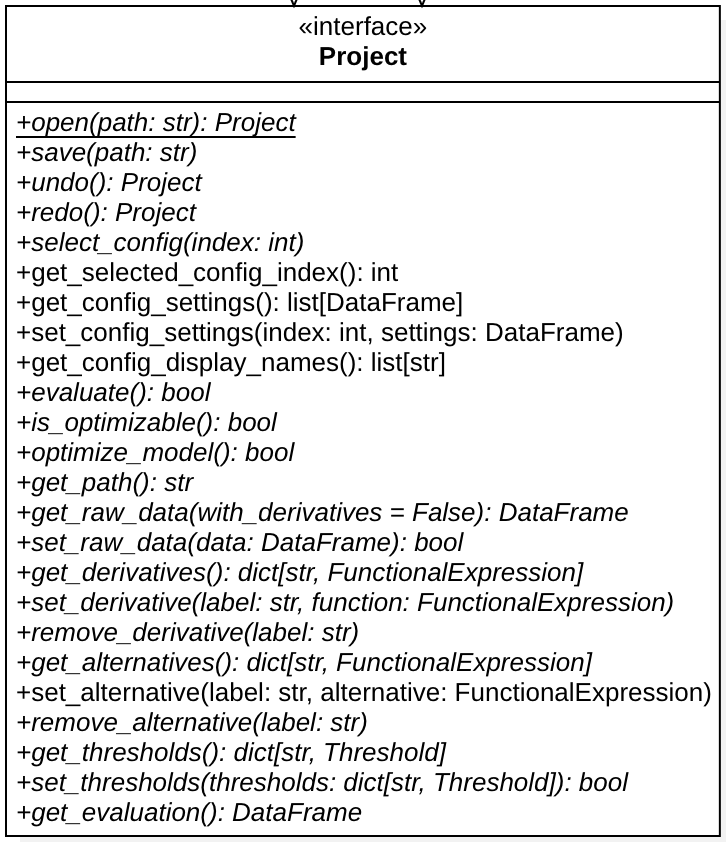
\includegraphics[width=13cm]{entwurf/Entwurf_dokument/img/cls/model/Project.png}
    \caption{Klassendiagramm von \texttt{Project}}
\end{figure}

Das Interface stellt die Schnittstelle zwischen Datenmodell (\emph{Model}) und Benutzeroberfläche (\emph{View} und \emph{Controller}) dar. Es beinhaltet alle benötigten Methoden zur vollständigen Verwaltung eines Projekts.
\\\\

\textbf{Methoden}
\begin{itemize}\setlength\itemsep{3em}
\item \textit{\flqq{}static\frqq} \texttt{\underline{open(path: str): Project}}\\\\
Lädt ein unter dem Dateipfad \texttt{path} gespeichertes Projekt.
\\\\
\underline{Parameter}\\
\begin{tabular}{lll}
 & \texttt{path} & Dateipfad des Projekts.\\
\end{tabular}

\underline{Rückgabewert}\\
\begin{tabular}{lll}
 & Interface des Projekts.\\
\end{tabular}

\underline{Exceptions}\\
\begin{tabular}{lll}
 & \texttt{ValueError} & Dateipfad ist ungültig.\\
 & \texttt{IOError} & Fehler bei I/O-Operation.\\
\end{tabular}


\item \textit{\flqq{}abstract\frqq} \texttt{\textit{save(path: str = None)}}\\\\
Speichert ein Projekt unter dem im Projekt hinterlegten Pfad. Ein für diesen Speichervorgang abweichender Pfad kann optional über den Parameter \texttt{path} angegeben werden.
\\\\
\underline{Parameter}\\
\begin{tabular}{lll}
 & \texttt{path} & Dateipfad des Projekts.\\
 && Standardmäßig auf \texttt{None}.\\
 && Falls Pfad \texttt{None} ist, wird der im Projekt hinterlegte Projektpfad verwendet.\\
\end{tabular}

\underline{Rückgabewert}\\
\begin{tabular}{lll}
 & Keine Rückgabe.\\
\end{tabular}

\underline{Exceptions}\\
\begin{tabular}{lll}
 & \texttt{ValueError} & Dateipfad ist ungültig.\\
 & \texttt{IOError} & Fehler bei I/O-Operation.\\
\end{tabular}


\item \textit{\flqq{}abstract\frqq} \texttt{\textit{undo(): Project}}\\\\
Macht die letzte Änderung am Projekt rückgängig und gibt die letzte Version zurück.
\\\\
\underline{Parameter}\\
\begin{tabular}{lll}
 & Keine Parameter.
\end{tabular}

\underline{Rückgabewert}\\
\begin{tabular}{lll}
 & Projekt-Interface des Projekts vor der zuletzt vor genommenen Operation.\\
\end{tabular}

\underline{Exceptions}\\
\begin{tabular}{lll}
 & \texttt{IndexError} & Keine Vorgängerversion hinterlegt.\\
\end{tabular}


\item \textit{\flqq{}abstract\frqq} \texttt{\textit{redo(): Project}}\\\\
Macht das letzte \texttt{undo()} rückgängig, sofern seitdem nichts am Projekt verändert wurde.
\\\\
\underline{Parameter}\\
\begin{tabular}{lll}
 & Keine Parameter.
\end{tabular}

\underline{Rückgabewert}\\
\begin{tabular}{lll}
 & Projekt-Interface des Projekts vor dem letzten \texttt{undo()}-Aufruf.\\
\end{tabular}

\underline{Exceptions}\\
\begin{tabular}{lll}
 & \texttt{IndexError} & Keine Nachfolgerversion hinterlegt.\\
\end{tabular}


\item \textit{\flqq{}abstract\frqq} \texttt{\textit{select\char`_config(index: int)}}\\\\
Wählt die Konfiguration mit dem Index \texttt{index} aus der im Projekt hinterlegten Liste an Verarbeitungskonfigurationen (\texttt{ProcessingConfig}) für eine spätere Verarbeitung aus.
\\\\
\underline{Parameter}\\
\begin{tabular}{lll}
 & \texttt{index} & Index der gewünschten Konfiguration in der im Projekt hinterlegten Liste.
\end{tabular}

\underline{Rückgabewert}\\
\begin{tabular}{lll}
 & Keine Rückgabe.\\
\end{tabular}

\underline{Exceptions}\\
\begin{tabular}{lll}
 & \texttt{IndexError} & Index existiert nicht.\\
\end{tabular}

\item \textit{\flqq{}abstract\frqq} \texttt{\textit{select\char`_config(index: int)}}\\\\
Wählt die Konfiguration mit dem Index \texttt{index} aus der im Projekt hinterlegten Liste an Verarbeitungskonfigurationen (\texttt{ProcessingConfig}) für eine spätere Verarbeitung aus.
\\\\
\underline{Parameter}\\
\begin{tabular}{lll}
 & \texttt{index} & Index der gewünschten Konfiguration in der im Projekt hinterlegten Liste.
\end{tabular}

\underline{Rückgabewert}\\
\begin{tabular}{lll}
 & Keine Rückgabe.\\
\end{tabular}

\underline{Exceptions}\\
\begin{tabular}{lll}
 & \texttt{IndexError} & Index existiert nicht in hinterlegter Liste.\\
\end{tabular}


\item \textit{\flqq{}abstract\frqq} \texttt{\textit{get\char`_selected\char`_config\char`_index(): int}}\\\\
Getter für Index der gewählten Konfiguration aus der im Projekt hinterlegten Liste an Verarbeitungskonfigurationen (\texttt{ProcessingConfig}).
\\\\
\underline{Parameter}\\
\begin{tabular}{lll}
 & Keine Parameter.
\end{tabular}

\underline{Rückgabewert}\\
\begin{tabular}{lll}
 & Index der gewählten Konfiguration.\\
\end{tabular}


\item \textit{\flqq{}abstract\frqq} \texttt{\textit{get\char`_config\char`_settings(): list[pandas.DataFrame]}}\\\\
Getter für eine Liste aller im Projekt hinterlegten Einstellungen von Verarbeitungskonfigurationen (\texttt{settings} Attribut in \texttt{ProcessingConfig}).
\\\\
\underline{Parameter}\\
\begin{tabular}{lll}
 & Keine Parameter.
\end{tabular}

\underline{Rückgabewert}\\
\begin{tabular}{lll}
 & Liste aller hinterlegten Einstellungen von Verarbeitungskonfigurationen.\\
 & (\texttt{settings} Attribut in \texttt{ProcessingConfig}).\\
\end{tabular}


\item \textit{\flqq{}abstract\frqq} \texttt{\textit{get\char`_config\char`_settings(): list[pandas.DataFrame]}}\\\\
Getter für eine Liste aller im Projekt hinterlegten Einstellungen von Verarbeitungskonfigurationen (\texttt{ProcessingConfig.settings}).
\\\\
\underline{Parameter}\\
\begin{tabular}{lll}
 & Keine Parameter.
\end{tabular}

\underline{Rückgabewert}\\
\begin{tabular}{lll}
 & Liste aller hinterlegten Einstellungen von Verarbeitungskonfigurationen\\
 & (\texttt{ProcessingConfig.settings}).\\
 & Das Orginalobjekt kann über den Rückgabewert nicht modifiziert werden.\\
\end{tabular}


\item \textit{\flqq{}abstract\frqq} \texttt{\textit{set\char`_config\char`_settings\char`_index(index: int, settings: pandas.DataFrame)}}\\\\
Setter für Einstellungen von im Projekt hinterlegten Verarbeitungskonfigurationen (\texttt{ProcessingConfig}).
\\\\
\underline{Parameter}\\
\begin{tabular}{lll}
 & \texttt{index} & Index der Verarbeitungskonfiguration,\\
 && zu der die Einstellungen geändert werden sollen.\\
 & \texttt{settings} & Neue zu setzenden Einstellungen\\
\end{tabular}

\underline{Rückgabewert}\\
\begin{tabular}{lll}
 & Index der gewählten Konfiguration.\\
\end{tabular}


\item \textit{\flqq{}abstract\frqq} \texttt{\textit{get\char`_config\char`_display\char`_names(): list[str]}}\\\\
Getter für eine Liste der Anzeigenamen von allen im Projekt hinterlegten Verarbeitungskonfigurationen (\texttt{ProcessingConfig}).
\\\\
\underline{Parameter}\\
\begin{tabular}{lll}
 & Keine Parameter.
\end{tabular}

\underline{Rückgabewert}\\
\begin{tabular}{lll}
 & Liste der Anzeigenamen.\\
 & Das Orginalobjekt kann über den Rückgabewert nicht modifiziert werden.\\
\end{tabular}


\item \textit{\flqq{}abstract\frqq} \texttt{\textit{evaluate(): bool}}\\\\
Führt das im Projekt konfigurierte Verarbeitungsverfahren aus.
\\\\
\underline{Parameter}\\
\begin{tabular}{lll}
 & Keine Parameter.\\
\end{tabular}

\underline{Rückgabewert}\\
\begin{tabular}{lll}
 & Wahrheitswert, ob Auswertung erfolgreich war.\\
\end{tabular}

\underline{Exceptions}\\
\begin{tabular}{lll}
 & \texttt{ValueError} & Voraussetzungen für eine Berechnung sind nicht erfüllt.\\
\end{tabular}


\item \textit{\flqq{}abstract\frqq} \texttt{\textit{is\char`_optimizable(): bool}}\\\\
Prüft, ob zurzeit eine Modelloptimierung prinzipiell möglich ist.\\\\
\underline{Parameter}\\
\begin{tabular}{lll}
 & Keine Parameter.
\end{tabular}

\underline{Rückgabewert}\\
\begin{tabular}{lll}
 & Wahrheitswert, ob Optimierung prinzipiell möglich ist. Dies ist der Fall, wenn eine optimierbare Auswertung existiert.\\
\end{tabular}


\item \textit{\flqq{}abstract\frqq} \texttt{\textit{optimize\char`_model(): bool}}\\\\
Führt eine Modelloptimierung auf Grundlage einer zuvor angefertigten Auswertung aus.
\\\\
\underline{Parameter}\\
\begin{tabular}{lll}
 & Keine Parameter.\\
\end{tabular}

\underline{Rückgabewert}\\
\begin{tabular}{lll}
 & Wahrheitswert, ob Optimierung erfolgreich war.\\
\end{tabular}

\underline{Exceptions}\\
\begin{tabular}{lll}
 & \texttt{ValueError} & Voraussetzungen für eine Berechnung sind nicht erfüllt.\\
\end{tabular}


\item \textit{\flqq{}abstract\frqq} \texttt{\textit{get\char`_path(): str}}\\\\
Getter für den Projektdateipfad, an dem das Projekt standardmäßig (u.~a. automatisch) gespeichert wird.
\\\\
\underline{Parameter}\\
\begin{tabular}{lll}
 & Keine Parameter.
\end{tabular}

\underline{Rückgabewert}\\
\begin{tabular}{lll}
 & Projektdateipfad.\\
\end{tabular}


\item \textit{\flqq{}abstract\frqq} \texttt{\textit{get\char`_raw\char`_data(with\char`_derivatives = False): pandas.DataFrame}}\\\\
Getter für eine Liste der im Projekt importierten Rohdaten / Umfragedaten. Bei Bedarf werden auch Spaltenableitungen hinzugefügt.
\\\\
\underline{Parameter}\\
\begin{tabular}{lll}
 & \texttt{with\char`_derivatives} & Gibt an, ob Spaltenableitungen ebenfalls berechnet\\
 && und zur Rückgabe hinzugefügt werden sollen.\\
 && Standardwert ist \texttt{False}.\\
\end{tabular}

\underline{Rückgabewert}\\
\begin{tabular}{lll}
 & Tabelle der Rohdaten.\\
 & Das Orginalobjekt kann über den Rückgabewert nicht modifiziert werden.\\
\end{tabular}

\underline{Exceptions}\\
\begin{tabular}{lll}
 & \texttt{Exception} & Spaltenableitungen konnten nicht korrekt gebildet werden\\
 && (\texttt{with\char`_derivatives = True}).\\
\end{tabular}


\item \textit{\flqq{}abstract\frqq} \texttt{\textit{set\char`_raw\char`_data(data: pandas.DataFrame)}}\\\\
Setter für die im Projekt hinterlegten Rohdaten / Umfragedaten.
\\\\
\underline{Parameter}\\
\begin{tabular}{lll}
 & \texttt{data} & Neuer zu setzender Rohdatensatz.\\
\end{tabular}

\underline{Rückgabewert}\\
\begin{tabular}{lll}
 & Keine Rückgabe.\\
\end{tabular}


\item \textit{\flqq{}abstract\frqq} \texttt{\textit{get\char`_derivatives(): dict[str, FunctionalExpression]}}\\\\
Getter für alle definierten Spaltenableitungsfunktionen.
\\\\
\underline{Parameter}\\
\begin{tabular}{lll}
 & Keine Parameter.\\
\end{tabular}

\underline{Rückgabewert}\\
\begin{tabular}{lll}
 & Dictionary mit Ableitungsbezeichner als Schlüssel und \texttt{FunctionalExpression}\\
 & als zugeordneter Wert.\\
 & Das Orginalobjekt kann über den Rückgabewert nicht modifiziert werden.\\
\end{tabular}


\item \textit{\flqq{}abstract\frqq} \texttt{\textit{set\char`_derivative(label: str, function: FunctionalExpression)}}\\\\
Setter für im Projekt hinterlegte Spaltenableitungen.
\\\\
\underline{Parameter}\\
\begin{tabular}{lll}
 & \texttt{label} & Bezeichner der zu setzende Spaltenableitung.\\
 & \texttt{function} & Ableitungsfunktion als \texttt{FunctionalExpression}.\\
\end{tabular}

\underline{Rückgabewert}\\
\begin{tabular}{lll}
 & Keine Rückgabe.\\
\end{tabular}


\item \textit{\flqq{}abstract\frqq} \texttt{\textit{remove\char`_derivative(label: str)}}\\\\
Setter für im Projekt hinterlegten Spaltenableitungen.
\\\\
\underline{Parameter}\\
\begin{tabular}{lll}
 & \texttt{label} & Bezeichner der zu löschenden Spaltenableitung.\\
\end{tabular}

\underline{Rückgabewert}\\
\begin{tabular}{lll}
 & Keine Rückgabe.\\
\end{tabular}

\underline{Exceptions}\\
\begin{tabular}{lll}
 & \texttt{ValueError} & Ableitungsbezeichner ist ungültig.\\
\end{tabular}


\item \textit{\flqq{}abstract\frqq} \texttt{\textit{import\char`_derivative\char`(path: str)}}\\\\
Importiert eine Spaltenableitungsfunktionen aus einer Datei in das Projekt.
\\\\
\underline{Parameter}\\
\begin{tabular}{lll}
 & \texttt{path} & Dateipfad an dem die Spaltenableitung gespeichert ist.\\
\end{tabular}

\underline{Rückgabewert}\\
\begin{tabular}{lll}
 & Keine Rückgabe.\\
\end{tabular}

\underline{Exceptions}\\
\begin{tabular}{lll}
 & \texttt{ValueError} & Dateipfad ist ungültig.\\
 & \texttt{IOError} & Fehler bei I/O-Operation.\\
\end{tabular}


\item \textit{\flqq{}abstract\frqq} \texttt{\textit{export\char`_derivative(label: str, path: str)}}\\\\
Exportiert eine im Projekt hinterlegte Spaltenableitungsfunktionen.
\\\\
\underline{Parameter}\\
\begin{tabular}{lll}
 & \texttt{label} & Bezeichner der zu exportierenden Spaltenableitung.\\
 & \texttt{path} & Dateipfad an dem die Spaltenableitung gespeichert wird.\\
\end{tabular}

\underline{Rückgabewert}\\
\begin{tabular}{lll}
 & Keine Rückgabe.\\
\end{tabular}

\underline{Exceptions}\\
\begin{tabular}{lll}
 & \texttt{ValueError} & Ableitungsbezeichner oder Dateipfad ist ungültig.\\
 & \texttt{IOError} & Fehler bei I/O-Operation.\\
\end{tabular}


\item \textit{\flqq{}abstract\frqq} \texttt{\textit{get\char`_derivative\char`_error\char`_report(label: str): ErrorReport}}\\\\
Erstellt einen Fehlerbericht zu einer Spaltenableitungsfunktion.
\\\\
\underline{Parameter}\\
\begin{tabular}{lll}
 & \texttt{label} & Bezeichner der zu prüfenden Spaltenableitung.\\
\end{tabular}

\underline{Rückgabewert}\\
\begin{tabular}{lll}
 & Fehlerbericht in Form eines \texttt{ErrorReport}-Objekts.\\
\end{tabular}

\underline{Exceptions}\\
\begin{tabular}{lll}
 & \texttt{ValueError} & Ableitungsbezeichner ist ungültig.\\
\end{tabular}


\item \textit{\flqq{}abstract\frqq} \texttt{\textit{get\char`_alternatives(): dict[str, FunctionalExpression]}}\\\\
Getter für alle definierten Nutzenfunktionen.
\\\\
\underline{Parameter}\\
\begin{tabular}{lll}
 & Keine Parameter.\\
\end{tabular}

\underline{Rückgabewert}\\
\begin{tabular}{lll}
 & Dictionary mit Alternativenbezeichner als Schlüssel und \texttt{FunctionalExpression}\\
 & als zugeordneter Wert.\\
 & Das Orginalobjekt kann über den Rückgabewert nicht modifiziert werden.\\
\end{tabular}



\item \textit{\flqq{}abstract\frqq} \texttt{\textit{set\char`_alternative(label: str, function: FunctionalExpression)}}\\\\
Setter für im Projekt hinterlegte Nutzenfunktionen.
\\\\
\underline{Parameter}\\
\begin{tabular}{lll}
 & \texttt{label} & Bezeichner der zu setzenden Spaltenableitung.\\
 & \texttt{function} & Ableitungsfunktion als \texttt{FunctionalExpression}.\\
\end{tabular}

\underline{Rückgabewert}\\
\begin{tabular}{lll}
 & Keine Rückgabe.\\
\end{tabular}


\item \textit{\flqq{}abstract\frqq} \texttt{\textit{remove\char`_alternative(label: str)}}\\\\
Löscht eine im Projekt hinterlegte Nutzenfunktion.
\\\\
\underline{Parameter}\\
\begin{tabular}{lll}
 & \texttt{label} & Bezeichner der zu löschenden Spaltenableitung.\\
\end{tabular}

\underline{Rückgabewert}\\
\begin{tabular}{lll}
 & Keine Rückgabe.\\
\end{tabular}

\underline{Exceptions}\\
\begin{tabular}{lll}
 & \texttt{ValueError} & Ableitungsbezeichner ist ungültig.\\
\end{tabular}


\item \textit{\flqq{}abstract\frqq} \texttt{\textit{import\char`_alternative(path: str)}}\\\\
Importiert eine Nutzenfunktion aus einer Datei in das Projekt.
\\\\
\underline{Parameter}\\
\begin{tabular}{lll}
 & \texttt{path} & Dateipfad an dem die Nutzenfunktion gespeichert ist.\\
\end{tabular}

\underline{Rückgabewert}\\
\begin{tabular}{lll}
 & Keine Rückgabe.\\
\end{tabular}

\underline{Exceptions}\\
\begin{tabular}{lll}
 & \texttt{ValueError} & Dateipfad ist ungültig.\\
 & \texttt{IOError} & Fehler bei I/O-Operation.\\
\end{tabular}


\item \textit{\flqq{}abstract\frqq} \texttt{\textit{export\char`_alternative(label: str, path: str)}}\\\\
Exportiert eine im Projekt hinterlegte Nutzenfunktion.
\\\\
\underline{Parameter}\\
\begin{tabular}{lll}
 & \texttt{label} & Bezeichner der zu exportierenden Nutzenfunktion.\\
 & \texttt{path} & Dateipfad an dem die Nutzenfunktion gespeichert wird.\\
\end{tabular}

\underline{Rückgabewert}\\
\begin{tabular}{lll}
 & Keine Rückgabe.\\
\end{tabular}

\underline{Exceptions}\\
\begin{tabular}{lll}
 & \texttt{ValueError} & Bezeichner der Nutzenfunktion oder Dateipfad ist ungültig.\\
 & \texttt{IOError} & Fehler bei I/O-Operation.\\
\end{tabular}


\item \textit{\flqq{}abstract\frqq} \texttt{\textit{get\char`_alternative\char`_error\char`_report(label: str): ErrorReport}}\\\\
Erstellt einen Fehlerbericht zu einer Spaltenableitungsfunktion.
\\\\
\underline{Parameter}\\
\begin{tabular}{lll}
 & \texttt{label} & Bezeichner der zu prüfenden Nutzenfunktion.\\
\end{tabular}

\underline{Rückgabewert}\\
\begin{tabular}{lll}
 & Fehlerbericht in Form eines \texttt{ErrorReport}-Objekts.\\
\end{tabular}

\underline{Exceptions}\\
\begin{tabular}{lll}
 & \texttt{ValueError} & Bezeichner der Nutzenfunktion ist ungültig.\\
\end{tabular}


\item \textit{\flqq{}abstract\frqq} \texttt{\textit{get\char`_thresholds(): dict[str, Threshold]}}\\\\
Getter für die im Projekt hinterlegten Darstellungsschwellwerte.
\\\\
\underline{Parameter}\\
\begin{tabular}{lll}
 & Keine Parameter.\\
\end{tabular}

\underline{Rückgabewert}\\
\begin{tabular}{lll}
 & Dictionary mit Schwellwertbezeichner als Schlüssel und \texttt{Threshold}\\
 & als zugeordneter Wert.\\
\end{tabular}


\item \textit{\flqq{}abstract\frqq} \texttt{\textit{set\char`_thresholds(thresholds: dict[str, Threshold])}}\\\\
Setter für die im Projekt hinterlegten Darstellungsschwellwerte.
\\\\
\underline{Parameter}\\
\begin{tabular}{lll}
 & \texttt{thresholds} & Dictionary mit Schwellwertbezeichner als Schlüssel und \texttt{Threshold}\\
 && als zugeordneter Wert.\\
\end{tabular}

\underline{Rückgabewert}\\
\begin{tabular}{lll}
 & Dictionary mit Schwellwertbezeichner als Schlüssel und \texttt{Threshold}\\
 & als zugeordneter Wert.\\
\end{tabular}


\item \textit{\flqq{}abstract\frqq} \texttt{\textit{get\char`_evaluation(): Evaluation}}\\\\
Getter für eine zuvor berechnete und im Projekt hinterlegte Auswertung.
\\\\
\underline{Parameter}\\
\begin{tabular}{lll}
 & Keine Parameter.\\
\end{tabular}

\underline{Rückgabewert}\\
\begin{tabular}{lll}
 & Zuvor im Projekt hinterlegte Verarbeitungsauswertung.\\
\end{tabular}
\end{itemize}

%----------------------------------
\newpage
\classheader{ProjectSnapshot}\label{cls:ProjectSnapshot}
\begin{tabular}{lll}
 Superklassen: & \texttt{Project}\\
 Subklassen: & --
\end{tabular}\\
\begin{figure}[H]%
    \centering
    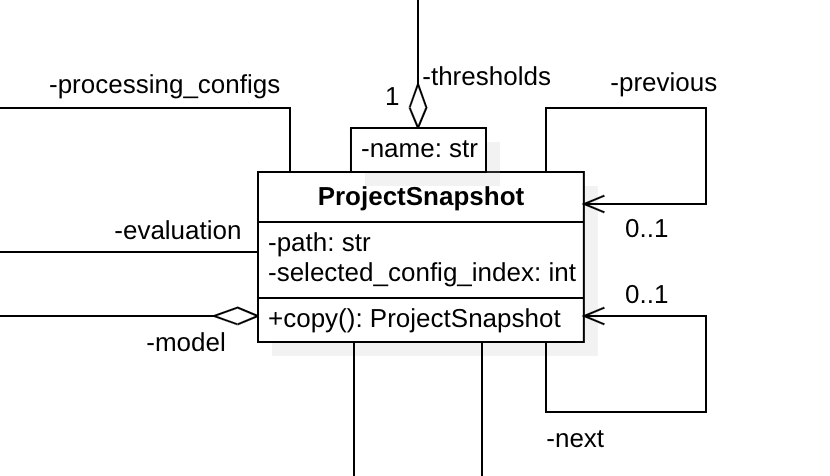
\includegraphics[width=13cm]{entwurf/Entwurf_dokument/img/cls/model/ProjectSnapshot.png}
    \caption{Klassendiagramm von \texttt{ProjectSnapshot}}
\end{figure}

Die Klasse repräsentiert einen Projektzustand zu einem bestimmten Zeitpunkt.
\\\\

\textbf{Attribute}
\begin{itemize}\setlength\itemsep{3em}
\item \texttt{path: str}\\\\
Dateipfad zum Projektverzeichnis, in dem das Projekt standardmäßig (u.~a. automatisch) gespeichert werden soll.
\item \texttt{previous: ProjectSnapshot}\\\\
Projektversion vor der letzten Daten-Operation, die auf dem Projekt durchgeführt wurde. Falls seit der letzten Widerrufs-Operation andere Daten-Operationen durchgeführt wurden, ist dieses Attribut \texttt{None}.
\item \texttt{next: ProjectSnapshot}\\\\
Projektversion vor der letzten Widerrufs-Operation (\texttt{undo()}), die auf dem Projekt durchgeführt wurde.
\item \texttt{model: Model}\\\\
Diskretes Wahlmodell, welches im Projekt definiert ist.
\item \texttt{processing\char`_configs: list[ProcessingConfig]}\\\\
Liste der im Projekt definierten Verarbeitungskonfigurationen (\texttt{ProcessingConfig}).
\item \texttt{selected\char`_config\char`_index: int}\\\\
Listenindex von \texttt{processing\char`_configs}. Das Listenelement ist die aktuell gewählte Verarbeitungskonfiguration (\texttt{ProcessingConfig}).
\item \texttt{evaluation: Evaluation}\\\\
Auswertung einer Datenverarbeitung, sofern durchgeführt. Ansonsten \texttt{None}.
\item \texttt{thesholds: dict[str, Threshold]}\\\\
Im Projekt konfigurierte Schwellwerte zur Hervorhebung einzelner Auswertungsdaten.
\\\\
\end{itemize}

\textbf{Methoden}
\begin{itemize}\setlength\itemsep{3em}
\item \texttt{copy(): ProjectSnapshot}\\\\
Erstellt eine Kopie des Objekts und gibt diese zurück.
\\\\
\underline{Parameter}\\
\begin{tabular}{lll}
 & Keine Parameter.
\end{tabular}

\underline{Rückgabewert}\\
\begin{tabular}{lll}
 & Kopie des Objekts.\\
\end{tabular}
\end{itemize}

%----------------------------------
\newpage
\classheader{ProxyProject}\label{cls:ProxyProject}
\begin{tabular}{lll}
 Superklassen: & \texttt{Project}\\
 Subklassen: & --
\end{tabular}\\
\begin{figure}[H]%
    \centering
    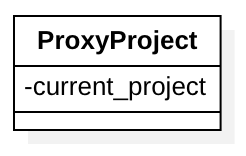
\includegraphics[width=13cm]{entwurf/Entwurf_dokument/img/cls/model/ProxyProject.png}
    \caption{Klassendiagramm von \texttt{ProxyProject}}
\end{figure}

Die Klasse dient entsprechend dem Proxy-Entwurfsmuster zur Erstellung einer zeitunabhängigen Schnittstelle zur Verwaltung eines Projekts. Dies ist notwendig, da die in \texttt{ProjectSnapshot} gehaltenen Daten nicht verändert werden dürfen, da diese als Historie erhalten bleiben sollen. Bei jeder Änderung wird ein neues \texttt{ProjectSnapshot}-Objekt erstellt. Mit dieser Historie werden dann z.~B. die Funktionen \texttt{undo()} und \texttt{redo()} realisiert. Die Proxy-Klasse verweist immer auf den aktuell gültigen \texttt{ProjectSnapshot}.
\\\\

\textbf{Attribute}
\begin{itemize}\setlength\itemsep{3em}
\item \texttt{current\char`_project: ProjectSnapshot}\\\\
Aktuell gültige Version des Projektinhalts.
\\\\
\end{itemize}

\textbf{Methoden}
\begin{itemize}\setlength\itemsep{3em}
\item[] Keine nicht-trivialen Methoden.
\end{itemize}

%----------------------------------
\newpage
\classheader[\flqq{}immutable\frqq]{Threshold}\label{cls:Threshold}
\begin{tabular}{lll}
 Superklassen: & --\\
 Subklassen: & --
\end{tabular}\\
\begin{figure}[H]%
    \centering
    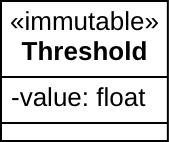
\includegraphics[width=13cm]{entwurf/Entwurf_dokument/img/cls/model/Threshold.png}
    \caption{Klassendiagramm von \texttt{Threshold}}
\end{figure}

Die Klasse repräsentiert einen Darstellungsschwellwert. Hierfür wurde eine eigene Klasse konsturiert, um Erweiterbarkeit zu ermöglichen.
\\\\

\textbf{Attribute}
\begin{itemize}\setlength\itemsep{3em}
\item \texttt{value: float}\\\\
Schwellwert.
\\\\
\end{itemize}

\textbf{Methoden}
\begin{itemize}\setlength\itemsep{3em}
\item[] Keine nicht-trivialen Methoden.
\end{itemize}
%--------------------------------------
\newpage
\subsection{Controller}

Im folgenden Abschnitt werden die Klassen des Paketes \emph{Controller}, so wie sie in Abb.~\ref{fig:ControllerKlassendiagramm} dargestellt sind, dokumentiert.

\begin{figure}[H]%
    \centering
    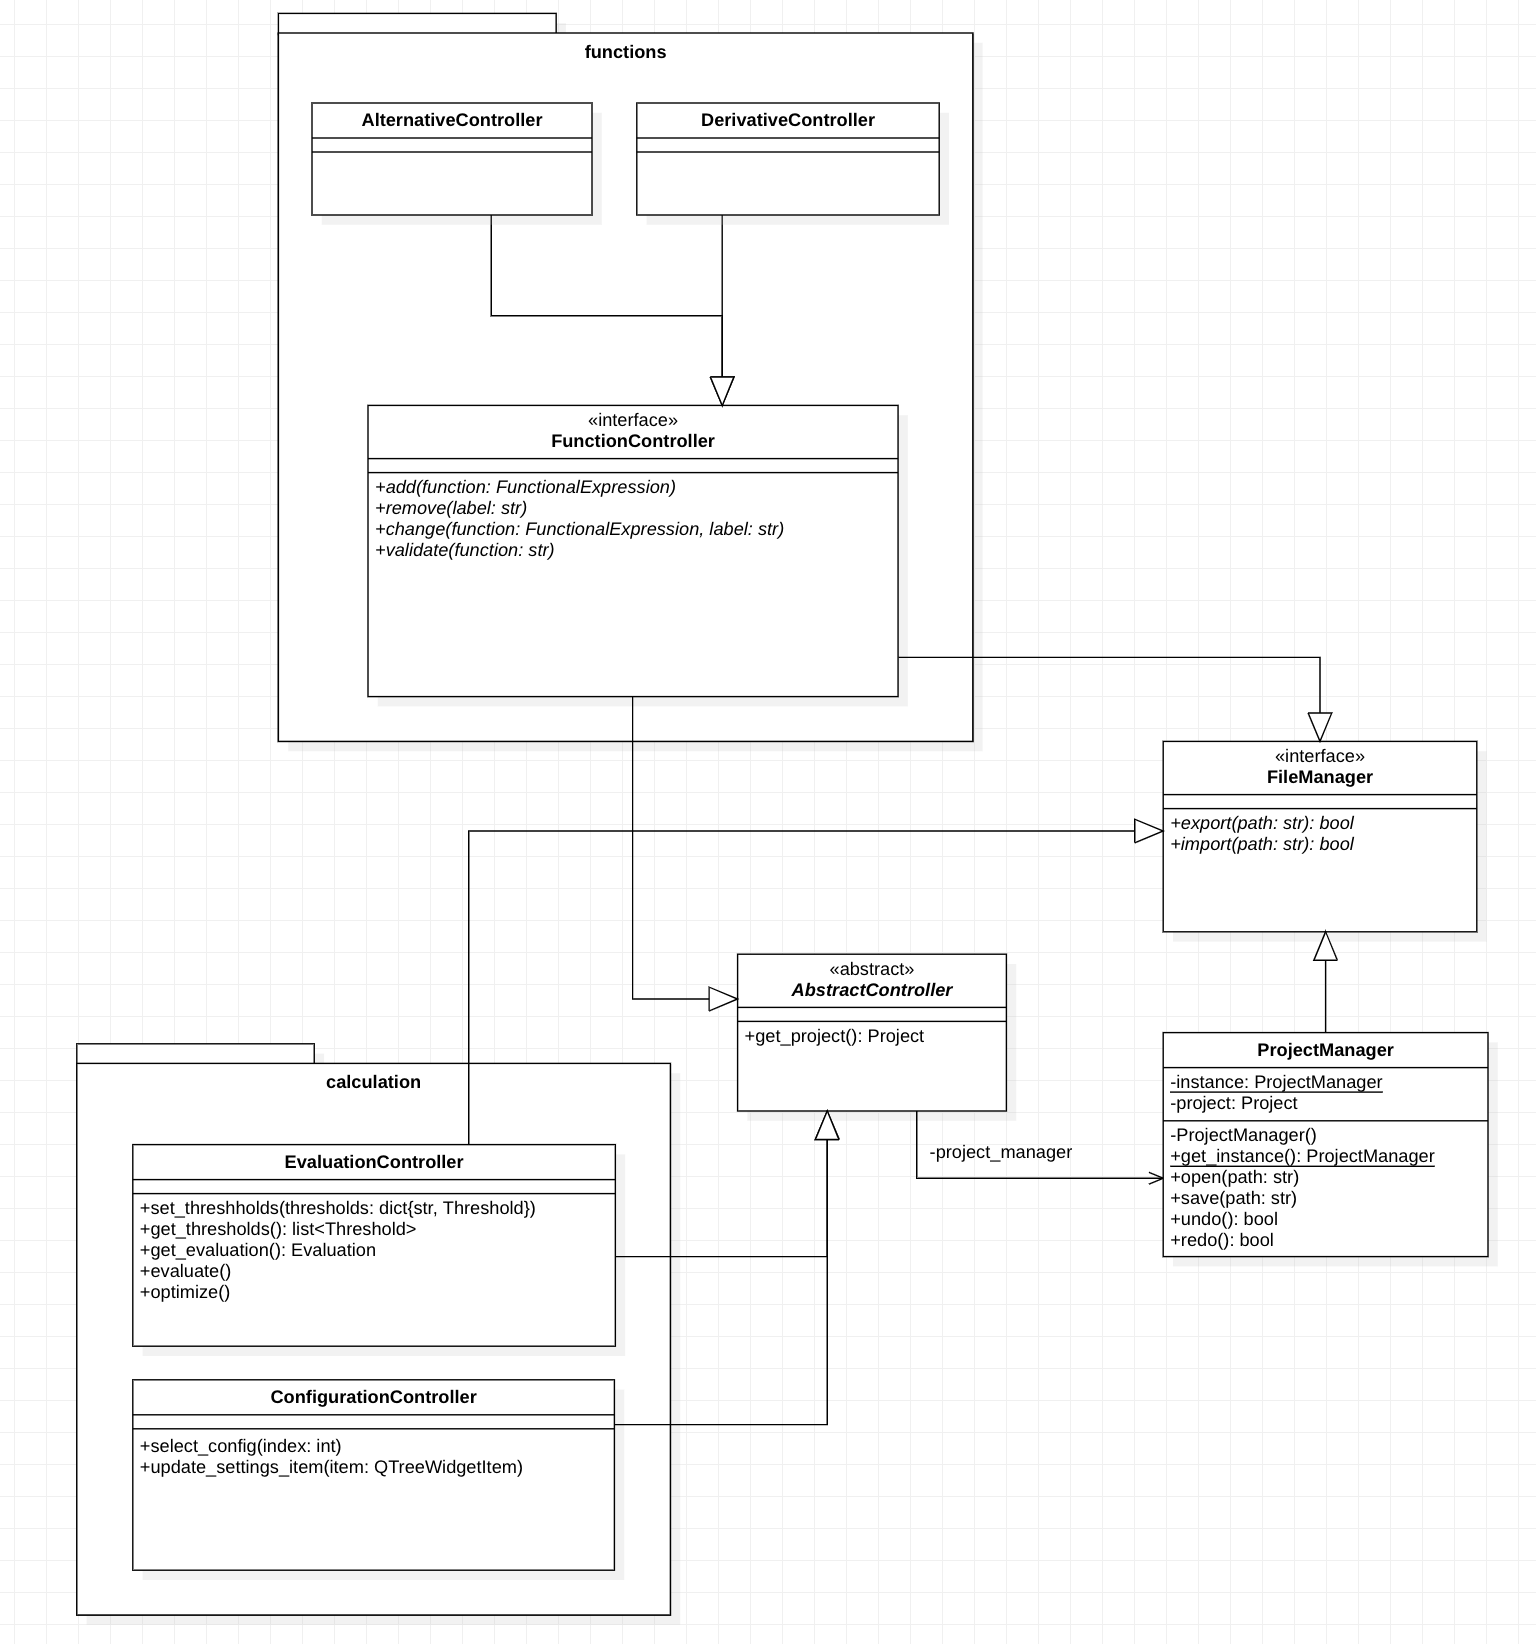
\includegraphics[width=13cm]{entwurf/Floriane/ControllerKlassendiagramm.png}
    \caption{Klassendiagramm Controller}
    \label{fig:ControllerKlassendiagramm}
\end{figure}

Das Package \textit{Controller} beinhaltet sechs Klassen und zwei Interfaces, die den 'Control'-Teil des Modells 'Model-View-Control' umsetzen.

\newpage
\classheader[\flqq{}interface\frqq]{FileManager}\label{cls:FileManager}
\begin{tabular}{lll}
 Superklassen: & --\\
 Subklassen: & \classref{ProjectManager} , \classref{FunctionController}, \classref{EvaluationController}
\end{tabular}\\

\begin{figure}[H]%
    \centering
    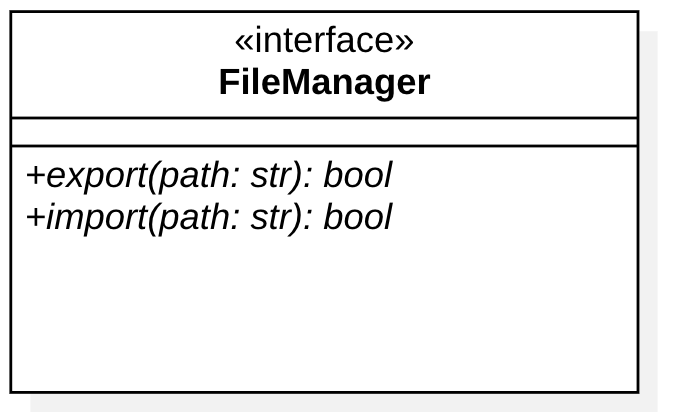
\includegraphics[width=6cm]{entwurf/Floriane/FileManager.png}
    \caption{Interface FileManager}
\end{figure}

Das Interface \textit{FileManager} dient der Interaktion mit externen Dateien. Es wird von allen Klassen im Controller implementiert. Es wurde in einem eigenen Interface entworfen, damit dieses später als Schnittstelle dienen kann, wenn Importe in und Exporte aus anderen Dateiformaten ermöglicht werden sollen.
\newline \newline
\textbf{{Methoden}}
\begin{itemize}
\item \textit{\flqq{}abstract\frqq} \texttt{import(path:str):bool} \newline Dient dem Import aller notwendigen Dateien und behandelt den Zugriff auf diese. Die Controller implementieren die Methode um sie für die jeweiligen Daten bzw. Funktionen zu nutzen.
\\\\
\underline{{Parameter}}

\begin{tabular}{lll}
 & \texttt{path:str} & Der Pfad zum Speicherort der zu importierenden Datei. \\
\end{tabular}

\underline{{Rückgabewert}}

\begin{tabular}{lll}
 & \texttt{bool} & Ob der Import erfolgreich war. \\
\end{tabular}

\item \textit{\flqq{}abstract\frqq}\texttt{export(path:str):bool} \newline Führt den Export einer Datei zu einem bestimmten Pfad aus. Diese Methode wird vom jeweiligen Controller implementiert.
\\\\
\underline{{Parameter}}

\begin{tabular}{lll}
 & \texttt{path:str} & Der Pfad zum Speicherort der zu speichernden Datei. \\
\end{tabular}

\underline{{Rückgabewert}}

\begin{tabular}{lll}
 & \texttt{bool} & Ob der Export erfolgreich war. \\
\end{tabular}
\end{itemize}



\newpage
\classheader{ProjectManager}\label{cls:ProjectManager}
\begin{tabular}{lll}
 Superklassen: & \classref{FileManager}\\
 Subklassen: & --
\end{tabular}\\
\begin{figure}[H]%
    \centering
    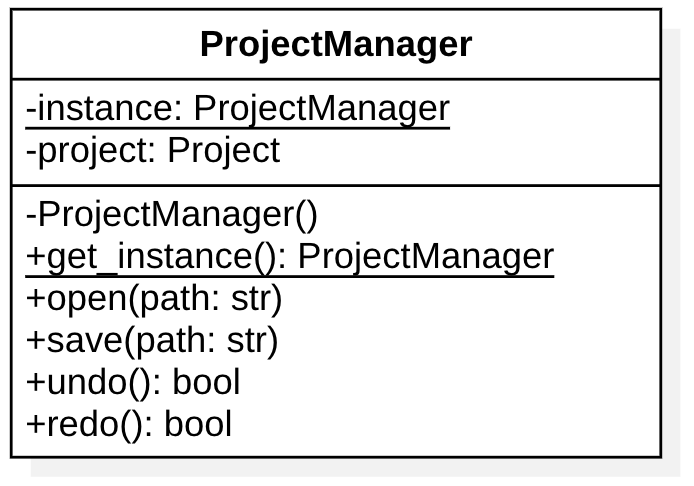
\includegraphics[width=7cm]{entwurf/Floriane/ProjectManager.png}
    \caption{Klasse ProjectManager}
\end{figure}

Der ProjectManager dient der Kontrolle der Project Objekte. Er wurde nach dem Muster des Singletons entworfen, indem er einen privaten Konstruktor hat, eine statische Instanz und eine statische Methode, die diese Instanz zurück gibt. So wird verhindert, dass es mehrere ProjektManager gibt, die möglicherweise auf verschiedene Projekte verweisen. Die anderen Controller erhalten Zugriff auf ihn durch die abstrakte Klasse AbstractController, die den ProjektManager als privates Attribut besitzt.
\newline\newline
\textbf{\large{Attribute}}
\begin{itemize}
\item \flqq{}static\frqq \texttt{instance: ProjectManager}\\ Die einzige Instanz dieser Klasse.
\item \texttt{project:Project}\\Private instanz der Klasse ProxyProject zur Projektverwaltung. Diese wird für alle Funktionen die das Projekt verändern und neue Snapshot. 
\end{itemize}\leavevmode\newline
\textbf{\large{Methoden}}
\begin{itemize}
\item \texttt{ProjectManager()}\\ Privater Konstruktor der Klasse zum Sicherstellen, dass es die Klasse nur eine Instanz besitzt.

\item \flqq{}static\frqq \texttt{get\_instance(): ProjectManager}\\ Zugriff auf den Projektmanager.\\\\
\underline{{Rückgabetypen}}\\
\begin{tabular}{llp{8.5cm}}
 & \texttt{ProjectManager} & Die einzige instanz des ProjektManagers. \\
\end{tabular}
\item \texttt{open(path:str)}\\ Öffnet ein neues oder bestehendes Projekt.\\\\
\underline{{Parameter}}\\
\begin{tabular}{llp{8.5cm}}
 & \texttt{path:str} & Der Pfand an dem das Projekt bereits besteht, oder das neue Projekt gespeichert werden soll. \\
\end{tabular}

\item \texttt{save(path:str)}\\ Speichern des Projektes.\\\\
\underline{{Parameter}}\\
\begin{tabular}{lll}
 & \texttt{path:str} & Der Pfad an dem das Projekt gespeichert werden soll. \\
\end{tabular}
\item \texttt{undo(): bool}\\ Rückgängigmachen der letzten Änderung. Im Projekt wird der aktuelle ProjectSnaphot durch den vorherigen ersetzt.\\\\
\underline{{Rückgabetypen}}\\
\begin{tabular}{lp{10.7cm}}
 & \texttt{bool}  True falls Änderung des Projektsnapshots erfolgreich war.\\
\end{tabular}
\item \texttt{redo(): bool): ProjectManager}\\ Wiederherstellen des zuletzt rückgängig gemachten Schrittes. Im Projekt wird der aktuelle Snapshot durch den folgenden ersetzt falls dieser existiert.\\\\
\underline{{Rückgabetypen}}\\
\begin{tabular}{lp{10.7cm}}
 & \texttt{bool}  True falls Änderung des Projektsnapshots erfolgreich war.\\
\end{tabular}
\end{itemize}


\newpage
\classheader[\flqq{}abstract\frqq]{AbstractController}\label{cls:AbstractController}
\begin{tabular}{lll}
 Superklassen: & -- \\
 Subklassen: & \classref{FunctionController}, \classref{EvaluationController}, \classref{ConfigurationController}
\end{tabular}\\
\begin{figure}[H]%
    \centering
    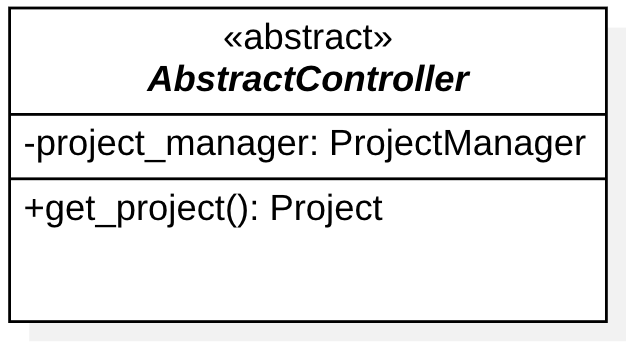
\includegraphics[width=6cm]{entwurf/Floriane/AbstractController.png}
    \caption{Abstrakte Klasse AbstractController}
\end{figure}


Abstrakte Klasse die als Verbindung zum ProjektManager dient. Die anderen Controller, die nicht für Speicherung oder Projektauswahl zuständig sind, können durch die geerbte Methode \texttt{get\_project()} auf das Projekt zugreifen. Da die Controller nicht das Attribut \texttt{project\_manager} erben, können sie den Projektmanager aber nicht ändern oder dessen Funktionen verwenden. Er dient in der Rolle Kollege zum 
Projektmanager im 'Vermittler' Entwurfsmuster.
\\\\
\textbf{\large{Attribute}}
\begin{itemize}
\item \texttt{project\_manager:ProjectManager}\\ Der Projektmanager des Programms. Dieser kann nicht neu gesetzt werden. Er ist privat, damit er nicht vererbt wird und die Kindklassen keinen direkten Zugriff besitzen.
\end{itemize}\leavevmode\newline
\textbf{\large{Methoden}}
\begin{itemize}
\item \texttt{get\_project():Project}\\ Methode als Schnittstelle zwischen den Controllern und dem Project aus dem Paket Model.\\\\
\underline{{Rückgabewert}}\\
\begin{tabular}{lll}
 & \texttt{Project} & Das aktuelle Projekt. \\
\end{tabular}
\end{itemize}



\newpage
\classheader[\flqq{}abstract\frqq]{FunctionController}\label{cls:FunctionController}
\begin{tabular}{lll}
 Superklassen: & \classref{AbstractController}, \classref{FileManager} \\
 Subklassen: & \classref{DerivativeController}, \classref{AlternativeController}
\end{tabular}\\

\begin{figure}[H]%
    \centering
    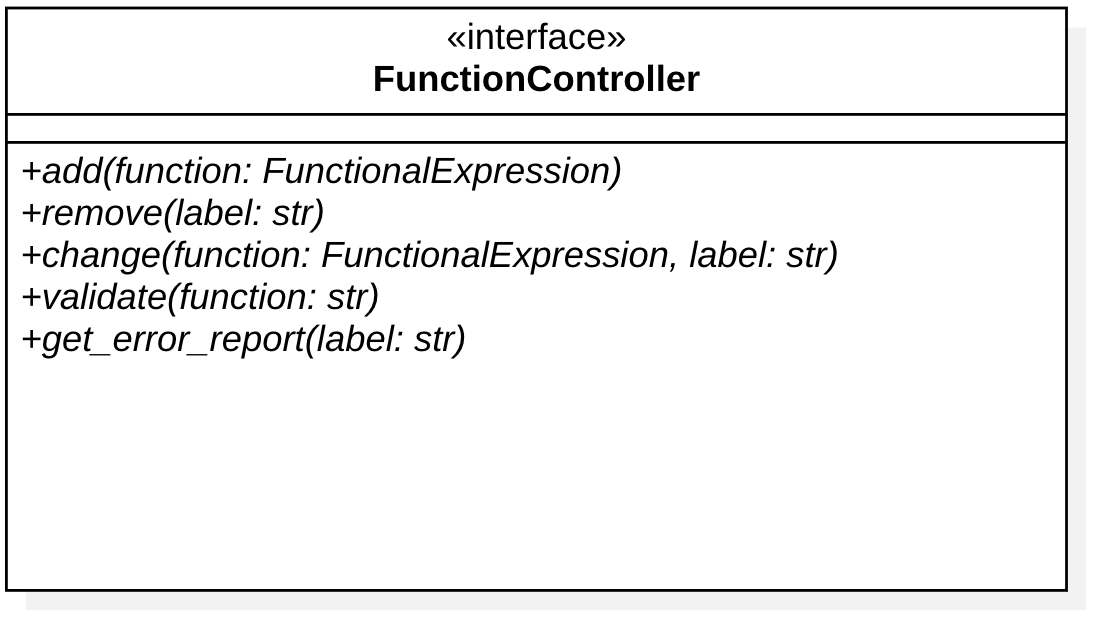
\includegraphics[width=10cm]{entwurf/Floriane/FunctionController.png}
    \caption{Abstrakte Klasse FunctionController}
\end{figure}


Controller Schablone zur Verwaltung der Funktionen. Das Interface besitzt die Funktionen die notwendigerweise von den konkreten Controllern zur Funktionsverwaltung implementiert werden müssen.
\newline\newline
\textbf{\large{Methoden}}
\begin{itemize}
\item \flqq{}abstract\frqq \texttt{add(label:str, function:FunctionalExpression)}\\ Hinzufügen neuer Funktionen zum aktuellen Projekt.\\\\
\underline{{Parameter}}\\
\begin{tabular}{lp{10.7cm}}
 & \texttt{function:FunctionalExpression}  Instanz der Klasse FunctionalExpression, die die Funktion die hinzugefügt werden soll enthält. \\
  & \texttt{label:str} Vom Nutzer gegebener Name der Funktion. \\
\end{tabular}
\item \flqq{}abstract\frqq \texttt{remove(label:str)}\\ Entfernung einer Funktion aus dem aktuellen Projekt. \\\\
\underline{{Parameter}}\\
\begin{tabular}{lll}
 & \texttt{label:str} & Name der Funktion zur Identifizierung im Model. \\
\end{tabular}
\item \flqq{}abstract\frqq \texttt{change(function:FunctionalExpression, label:str)}\\ Änderung einer Funktion im Projekt.\\\\
\underline{{Parameter}}\\
\begin{tabular}{lp{10.7cm}}
 & \texttt{function:FunctionalExpression}:  Neuer funktionaler Ausdruck als Instanz der Klasse FunctionalExpression.\\
 & \texttt{label:str}:  Name der Funkton zur Identifizierung im Model. \\
\end{tabular}
\item \flqq{}abstract\frqq \texttt{validate(function:str): FunctionalExpression}\\ Validierung der Nutzereingabe. Hier wird überprüft ob der Builder es der Klasse FunctionalExpression erlauben soll die Nutzereingabe als Python Code zu interpretieren. Code, der über einen mathematischen Ausdruck hinausgeht wird in dieser Methode abgefangen, bevor er evaluiert würde. Falls die Validierung erfolgreich ist, wird eine FunktionalExpression zurückgegeben. Falls nicht wird None zurückgegeben und die Nutzereingabe verworfen. Hier wird ausdrücklich nicht die Korrektheit des Funktionsausdrucks überprüft, sondern nur seine Existenz.\\\\
\underline{{Parameter}}\\
\begin{tabular}{lp{10.7cm}}
 & \texttt{function:str}  Nutzereingabe, die einen mathematischen Ausdruck wiederspiegeln soll. \\
\end{tabular}
\newline\newline
\underline{{Rückgabewert}}\\
\begin{tabular}{lp{10.7cm}}
 & \texttt{FunctionalExpression} Funktion als Objekt der Klasse FunctionalExpression so wie sie im Programm verarbeitet wird. \\
\end{tabular}


\item \flqq{}abstract\frqq \texttt{get\_error\_report(label:str)}\\ Ausführung der Evaluierung einer Funktion vom Controller aus. Dabei wird der zugrundeliegende mathematische Ausdruck evaluiert, sowie mögliche Fehler gefunden. Diese werden werden den Funktionenzugeordnet, sodass der View sie anzeigen kann. \\\\
\underline{{Parameter}}\\
\begin{tabular}{lp{10.7cm}}
 & \texttt{label:str} Name der Funktion, der dem Nutzer angezeigt wird. \\
\end{tabular}
\end{itemize}


\newpage
\classheader{AlternativeController}\label{cls:AlternativeController}
\begin{tabular}{lll}
 Superklassen: & \classref{FunctionController}\\
 Subklassen: & --
\end{tabular}\\
\begin{figure}[H]%
    \centering
    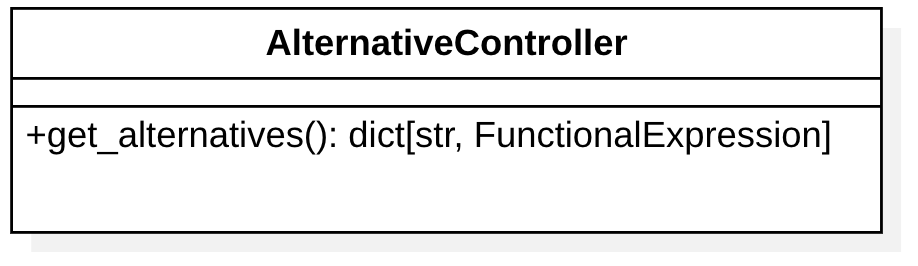
\includegraphics[width=10cm]{entwurf/Floriane/AlternativeController.png}
    \caption{AlternativeController}
\end{figure}

Die Klasse \textit{AlternativeController} ist zuständig für die Verwaltung der Alternativen. Sie implementiert das Interface \textit{FunctionController} mit den Funktionen add, change, remove und validate im Bezug auf die Alternativen.
\textbf{\large{Methoden}}
\begin{itemize}
\item \texttt{get\_alternatives(): dict[str, FunctionalExpression]}\\ Zugriff auf die im Projekt vorhandenen Alternativen.\\\\
\underline{{Rückgabetypen}}\\
\begin{tabular}{lp{10.7cm}}
 & \texttt{dict[str, FunctionalExpression]}  Dictionary mit allen Alternativen. Dabei sind die Namen der Alternativen die Schlüssel und die Funktionen in Form von FunctionalExpression Instanzen die Werte.\\
\end{tabular}
\end{itemize}


\newpage
\classheader{DerivativeController}\label{cls:DerivativeController}
\begin{tabular}{lll}
 Superklassen: & \classref{FunctionController}\\
 Subklassen: & --
\end{tabular}\\

\begin{figure}[H]%
    \centering
    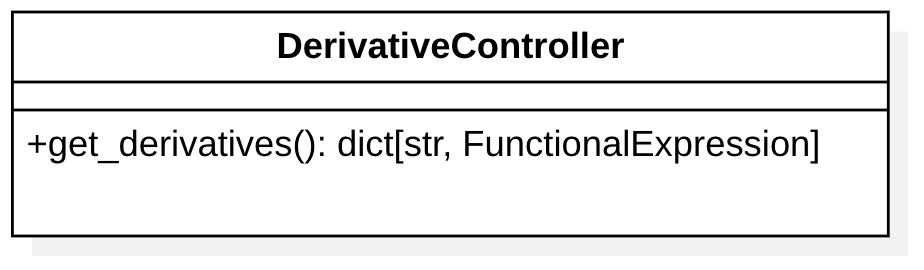
\includegraphics[width=10cm]{entwurf/Floriane/DerivativeController.png}
    \caption{DerivativeController}
\end{figure}

Die Klasse \textit{DerivativeController} ist zuständig für die Verwaltung der Attributsableitungsfunktionen. Sie implementiert das Interface \textit{FunctionController} mit den Funktionen add, change, remove und validate im Bezug auf die Attributsableitungsfunktionen.\\\\
\textbf{\large{Methoden}}
\begin{itemize}
\item \texttt{get\_derivatives(): dict[str, FunctionalExpression]}\\ Zugriff auf die im Projekt vorhandenen Attributsableitungen.\\\\
\underline{{Rückgabetypen}}\\
\begin{tabular}{lp{10.7cm}}
 & \texttt{dict[str, FunctionalExpression]}  Dictionary mit allen Attributsableitungsfunktionen. Dabei sind die Namen der Attribute die Schlüssel und die Funktionen in Form von FunctionalExpression Instanzen die Werte im Dictionary.\\
\end{tabular}
\end{itemize}

\newpage
\classheader{ConfigurationController}\label{cls:ConfigurationController}
\begin{tabular}{lll}
 Superklassen: & \classref{AbstractController}\\
 Subklassen: & --
\end{tabular}\\

\begin{figure}[H]%
    \centering
    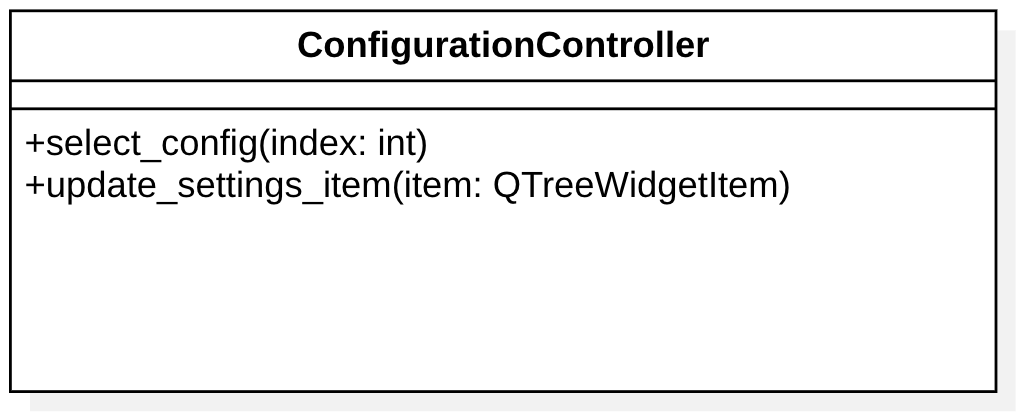
\includegraphics[width=10cm]{entwurf/Floriane/ConfigurationController.png}
    \caption{ConfigurationController}
\end{figure}

Verwaltet die Konfigurationen zur Modellberechnung. Es können die bereits implementierten Modell Konfigurationen aus einer Liste ausgewählt werden. \\\\
\textbf{\large{Methoden}}
\begin{itemize}
\item \texttt{select\_config(index:int)}\\ Methode zur Auswahl anderer Konfigurationen aus der Liste der bestehenden Konfigurationen.\\\\
\underline{{Parameter}}\\
\begin{tabular}{lp{10.7cm}}
 & \texttt{index:int} Index der ausgewählten Konfiguration in der Konfigurationsliste. \\
\end{tabular}
\item \texttt{update\_settings\_item(item: QTreeWidgetitem))}\\ Aktualisiert die Einstellungen im System entsprechend der Nutzereingaben im Frontend. Diese werden aus dem übergebenen Widget ausgelesen und in die ProcessingConfig übertragen.\\\\
\underline{{Parameter}}\\
\begin{tabular}{lp{10.7cm}}
 & \texttt{item:QTreeWidgetitem} Das Widget aus dem Frontend, das die Nutzereingaben enthält. \\
\end{tabular}
\end{itemize}


\newpage
\classheader{EvaluationController}\label{cls:EvaluationController}
\begin{tabular}{lll}
 Superklassen: & \classref{AbstractController}\\
 Subklassen: & --
\end{tabular}\\
\begin{figure}[H]%
    \centering
    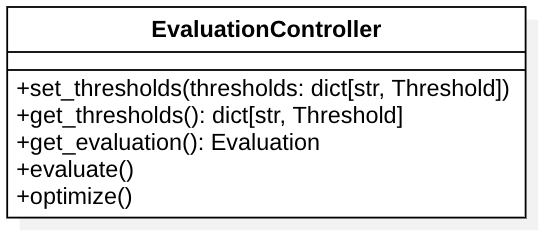
\includegraphics[width=10cm]{entwurf/Floriane/EvaluationController.png}
    \caption{EvaluationController}
\end{figure}

Kontrolle der Berechnungen des Programms. Ist zuständig für die Verwaltung der Schwellwerte, Modelloptimierungen und Evaluierungen.\\\\
\textbf{\large{Methoden}}
\begin{itemize}
\item \texttt{set\_thresholds(thresholds: dict{str, Threshold})}\\ Änderung der Schwellwerte, die im Programm hinterlegt sind.\\\\
\underline{{Parameter}}\\
\begin{tabular}{lp{10.7cm}}
 & \texttt{thresholds:dict[str,Threshold]} Dictionary, das die Namen der Schwellwarte als Schlüssel und die Schwellwertobjekte als Werte enthält. \\
\end{tabular}
\item \texttt{get\_thresholds(): dict[str, Threshold]}\\ Zugriffsmethode auf die Liste der Schwellwerte, die im Programmhinterlegt sind.\\\\
\underline{{Rückgabewerte}}\\
\begin{tabular}{lll}
 & \texttt{dict[str, Threshold]} & Liste aus Schwellwertobjekten. \\
\end{tabular}
\item \texttt{evaluate()}\\ Aufruf der Modellevaluierung im aktuellen Projekt.
\item \texttt{get\_evaluation():Evaluation}\\ Zugriff auf die bereits berechnete Modellevaluierung im aktuellen Projekt.\\\\
\underline{{Rückgabewerte}}\\
\begin{tabular}{lll}
 & \texttt{Evaluation} & Modellevaluierung, wie sie im Projekt berechnet wurde \\
\end{tabular}
\item \texttt{optimize()}\\ Methode zum Aufruf der Modelloptimierung im Projekt.\\
\end{itemize}





\newpage
\section{Softwareablauf}
\subsection{Projektmanagement}
\begin{figure}[H]%
    \centering
    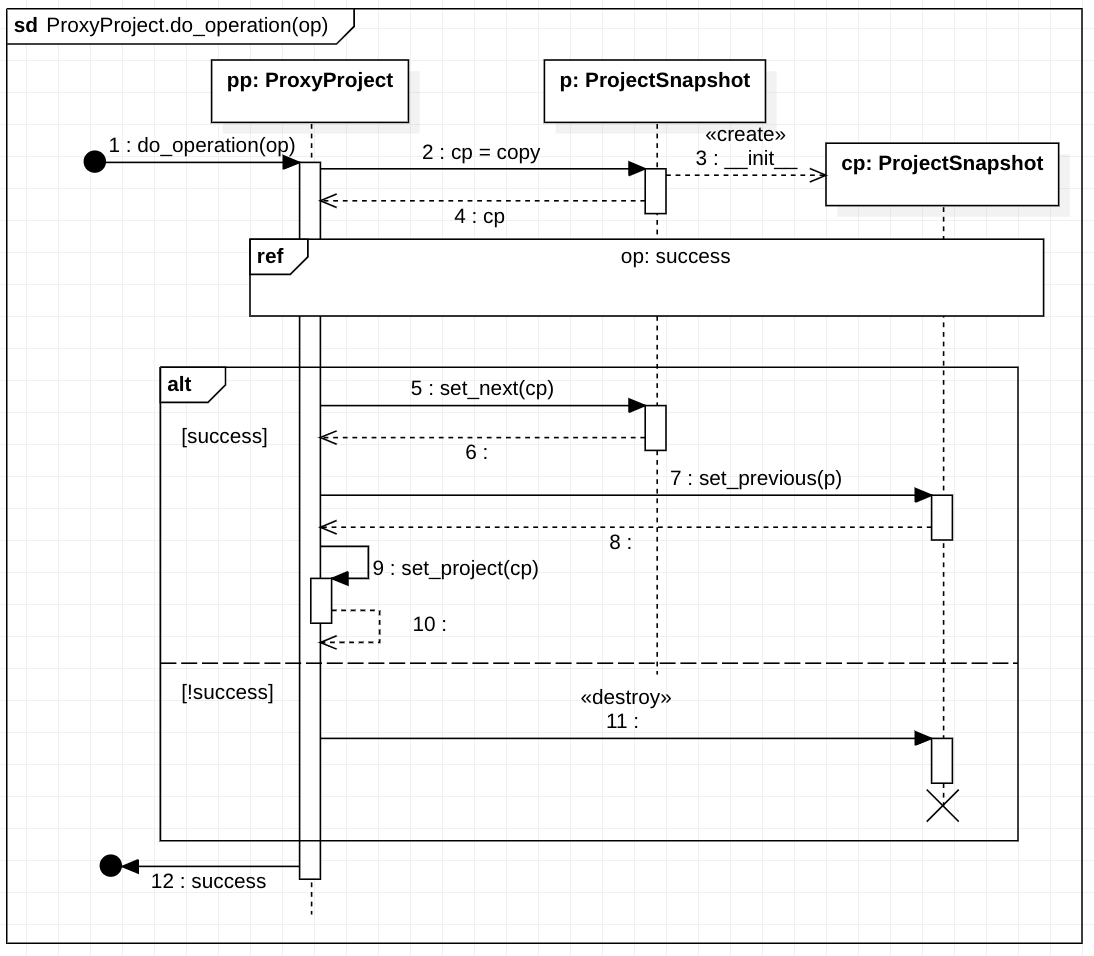
\includegraphics[width=13cm]{entwurf/Entwurf_dokument/img/Michael/sd_ProxyProject.do_operation.png}
    \caption{Sequenzdiagramm der Anwendung einer Projektoperation}
    \label{fig:sd:do_operation}
\end{figure}

Die Veränderung der Projektdaten ist Bestandteil jedes Anwendungsfalls. Aus diesem Grund bietet es sich an, für die Anwendung einer Projektoperation ein einheitliches Vorgehen zu entwerfen. Dieses ist in Abbildung \ref{fig:sd:do_operation} dargestellt.\\

\begin{enumerate}
    \item[1.] Befehl \texttt{do\char`_operation(op)} erreicht \texttt{pp:ProxyProject}
    \item[2.] Kopie des Projektzustands wird angestoßen
    \item[3.] Kopie des Projektzustands wird angelegt (\texttt{cp:ProjectSnapshot})
    \item[4.] Kopie wird an \texttt{ProxyProject} zurückgegeben
    \item[4.5.] Operation \emph{op} wird auf den neu angelegten Projektzustand (\emph{cp}) angewendet
    \item[] Wenn die Operation erfolgreich verlaufen ist:
    \begin{enumerate}
        \item[5.] Die neu angelegte Kopie (\emph{cp}) wird als Nachfolgezustand im alten Projektzustand (\emph{p}) hinterlegt.
        \item[7.] Im neuen Projektzustand (\emph{cp}) wird ebenso der alte Projektzustand als Vorgängerzustand (\emph{p}) hinterlegt.
        \item[9.] Wenn die Operation erfolgreich verlaufen ist, wird abschließend noch im \texttt{ProxyProject} (\emph{pp}) der neue Projektzustand (\emph{cp}) als aktueller Zustand hinterlegt.
    \end{enumerate}
    \item[] Wenn die Operation fehlgeschlagen ist:
    \begin{enumerate}
        \item[11.] Kopie des Projektzustands wird gelöscht.
    \end{enumerate}
    \item[12.] Zurückgeben, ob Operation erfolgreich.
    
\end{enumerate}

\textbf{\large{Neues Projekt öffnen}}
\begin{figure}[H]%
    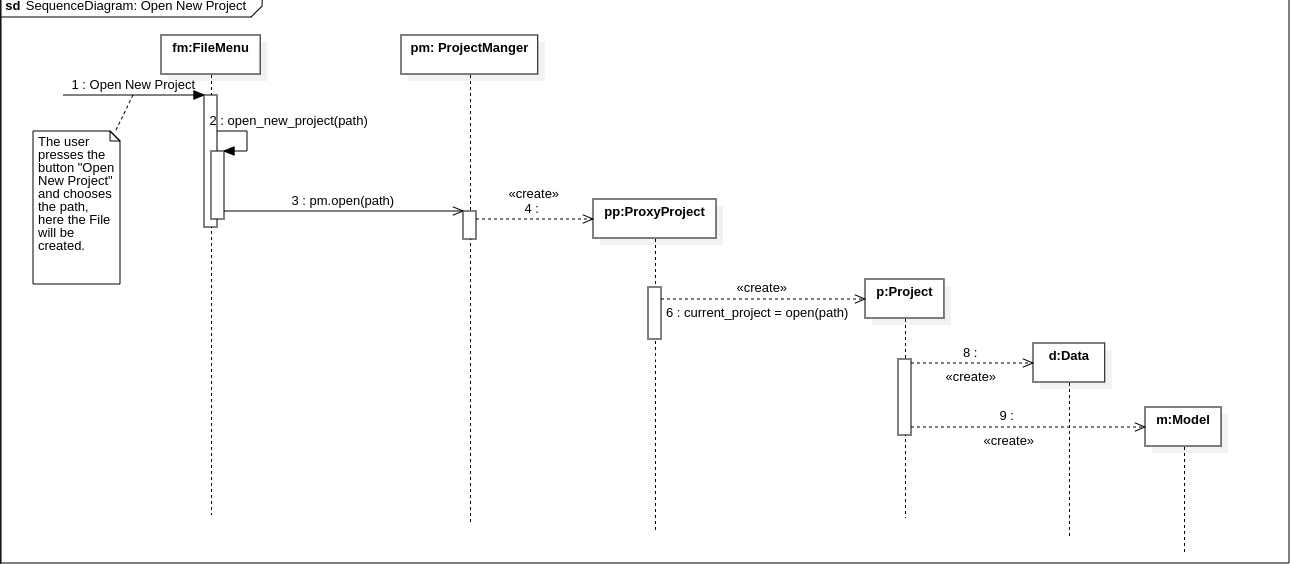
\includegraphics[width=15cm]{entwurf/Entwurf_dokument/img/Alissa/SQOpenNewProject3.png}
    \caption{Sequenzdiagramm für das Öffnen eines neuen Projektes}
    \label{fig:sd:openNewProject}
\end{figure}
Wenn ein Nutzer ein Projekt erstellen möchte, dann muss er zuerst ein neues Projekt erstellen lassen und dann die Erhebungsdaten importieren. Im folgenden wird die Sequenzdiagramm \ref{fig:sd:openNewProject} erläutert:

\begin{enumerate}
    \item[1.] Der Nutzer klickt auf die Schaltfläche 
    \enquote{Open New Project} im Dateimenü.
    \item[1.5] Der Nutzer wählt über dem Datei-Dialog den Speicherort.  
    \item[2.] Die Funktion \texttt{open\char`_new\char`_project(path)} in der Klasse \textit{FileMenu} aufgerufen. Als Parameter \textit{path} wird der gewählte Speicherort als String übergeben.
    \item[3.] In der Funktion \texttt{open\char`_new\char`_project(path)} wird der Controller(\textit{ProjectManager}) durch \texttt{open(path)} aufgerufen.
    \item[4.] Durch den Controller wird ein \textit{ProxyProject} Objekt erstellt.
    \item[5.] Der \textit{ProxyProject} Objekt erstellt automatisch (Mit aufrufen seiner Konstruktor) einen Objekt vom Typ \textit{Project}
    \item[6.] Der \textit{Project}\textendash Objekt erstellt widerrum Zwei Objekte. Einmal vom Typ \textit{Data} und dieser wird bei Erstellung des Objekts vom Typ \textit{Model} benötigt. 
\end{enumerate}

Somit wird ein neues Projekt geöffnet.
\begin{figure}[H]%
    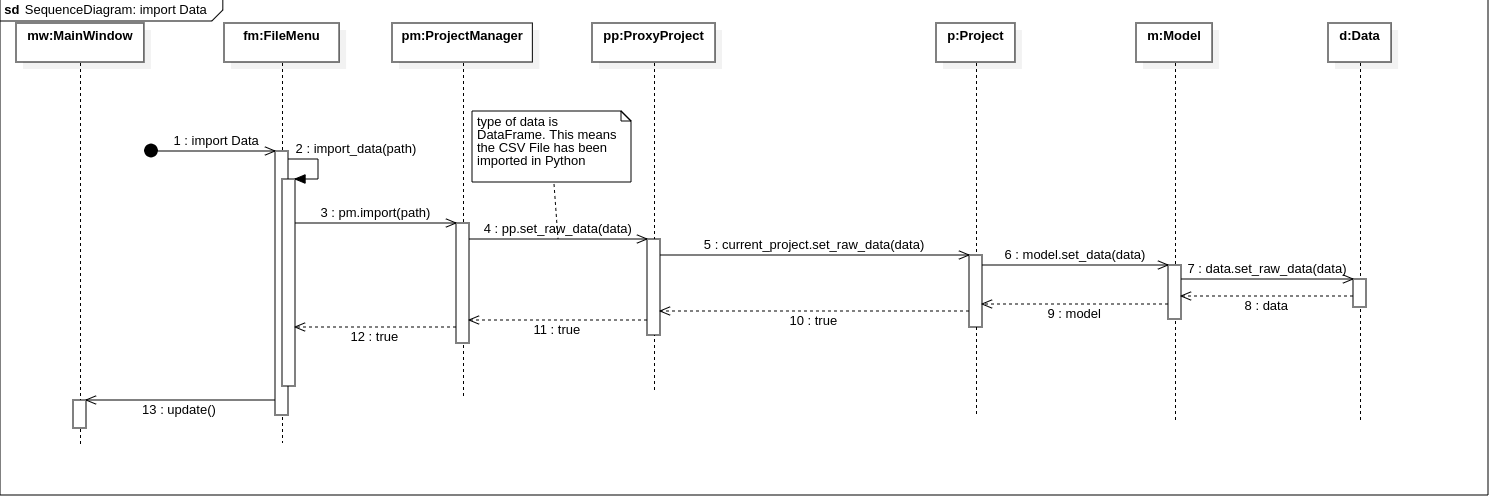
\includegraphics[width=15cm]{entwurf/Entwurf_dokument/img/Alissa/SQImportDataFinal.png}
    \caption{Sequenzdiagramm für den Import von Erhebungsdaten}
    \label{fig:sd:importData}
\end{figure}
Nun soll der Nutzer die Erhebungsdaten importieren wie in der Abbildung \ref{fig:sd:importData} beschrieben. Im folgenden wir der Ablauf erläutert:
\begin{enumerate}
    \item[1.] Der Nutzer klickt auf der Schaltfläche \enquote{Import Data} im \textit{File Menu} und wählt durch die Datei Dialog die zu importierenden CSV Datei. Dadurch wird die Funktion \texttt{import\char`_data(path)} im \hyperref[cls:FileMenu]{\textit{FileMenu}} aufgerufen.
    \item[2.] Dieser ruft den \hyperref[cls:ProjectManager]{ProjectManager}\textit{ProjectManager}, in dem die Methode \texttt{import()} aufgerufen wird.
    \item[3.] In der Methode \textit{import()} wird die CSV Datei geöffnet. Nun stehen die Daten als \textit{data} vom typ \textit{DataFrame}
    \item[4.] Die Daten werden an dem \textit{ProxyProject} übergeben, dieser ordnet dem \textit{Project}\textendash Objekt die Daten \textit{data} zu.
    \item[5.] Der \textit{Project}\textendash Objekt leitet die Daten an dem \textit{Model} weiter, und diese werden dann an dem \textit{Data} weitergeleitet. Dadurch wird es möglich, die Daten zu verwalten.
    \item[6.] Als letzter Schritt muss noch die \textit{FileMenu} die \textit{MainWindow} informieren, damit dieser die importierte Daten anzeigt. 
\end{enumerate}
\newpage
\textbf{\large{Projekt Öffnen}}
\begin{figure}[H]%
    \centering
    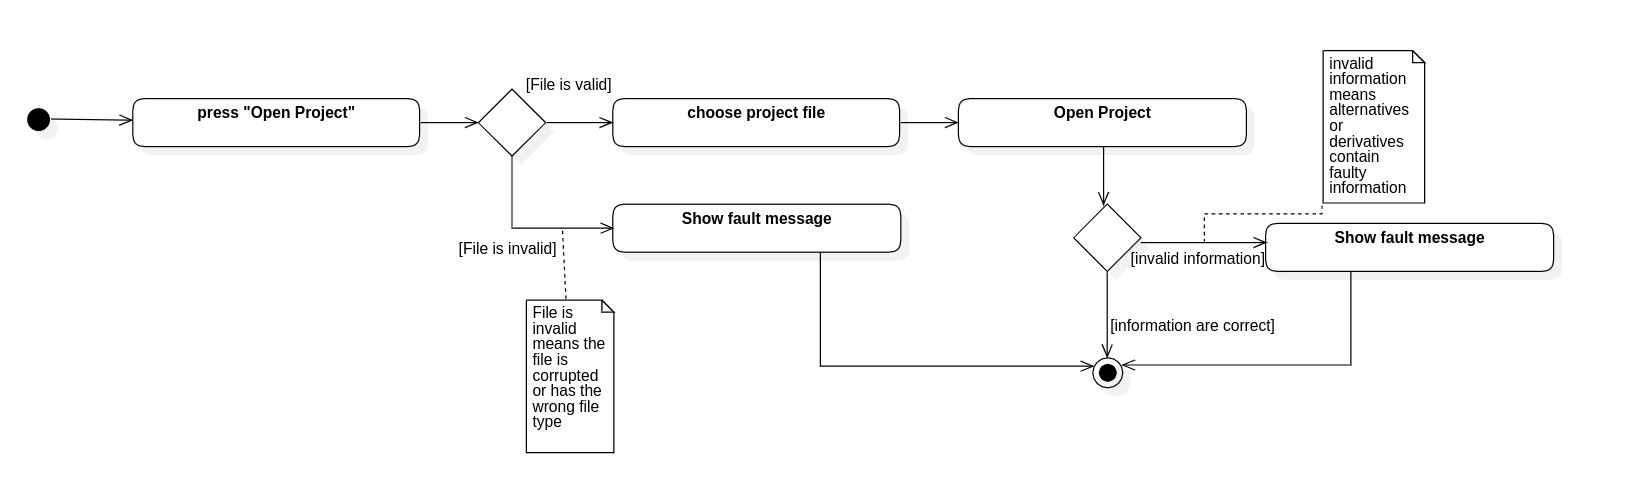
\includegraphics[width=13cm]{entwurf/Entwurf_dokument/img/Alissa/OpenProjectAD.png}
    \caption{Aktivitätsdiagramm Projekt öffnen}
    \label{ADProjektÖffnen}
\end{figure}
Der Nutzer kann auch ein Projekt öffnen, den er vorher erstellt hat. Dafür macht er folgendes \ref{ADProjektÖffnen}:
\begin{enumerate}
    \item[1.] er klickt auf \enquote{Open Project}. Diese befindet sich in der Dateimenü (engl. File Menu).
    \item[2.] Sollte die Datei valide sein. Das heißt es die Datei ist nicht korrupt und entspricht den erwarteten Dateityp, dann wird das Projekt geöffnet.
    \item[3.] Ansonsten erscheint eine Fehler Meldung und der Vorgang wird abgeborechen.
    \item[4.] Nach dem der Projekt geöffnet wurde, wird der Nutzer über Fehlerhafte Daten (Alternativen oder Ableitungen) informiert, falls es welche gibt. 
\end{enumerate}

\textbf{\large{Projekt Speichern}}
\begin{figure}[H]%
    \centering
    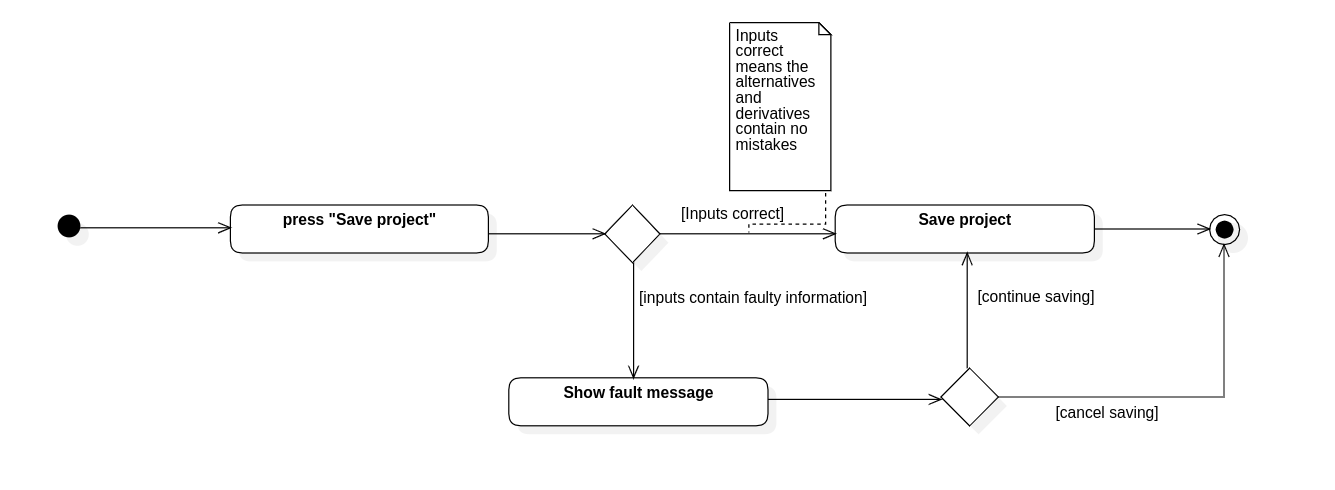
\includegraphics[width=13cm]{entwurf/Entwurf_dokument/img/Alissa/SaveProjectAD.png}
    \caption{Aktivitätsdiagramm für Projekt speichern}
    \label{ADProjekt Speichern}
\end{figure}
Damit der Nutzer den Projekt speichert, macht er folgendes \ref{ADProjekt Speichern}:
\begin{enumerate}
    \item[1.] Der Nutzer klickt auf \enquote{Save Project}, welcher in der Dateimenü zu finden ist.
    \item[2.] Wenn alle Nutzer Eingaben (Ableitungen und Alternativen) Korrekt sind, dann wird das Projekt gespeichrt.
    \item[3.] Ansonsten wird der Nutzer über die Existenz von fehlerhaften Eingaben informiert.
    \item[3.] Der Nutzer kann den Projekt trotz die Fehler speichern oder er bricht den vorgang ab.
\end{enumerate}
Alternativ kann der Nutzer auch einen anderen Speicherort wählen \ref{ADProkjektSpeichernAls}, anstatt die aktuelle Speicherort des projekts.

\begin{figure}[H]%
    \centering
    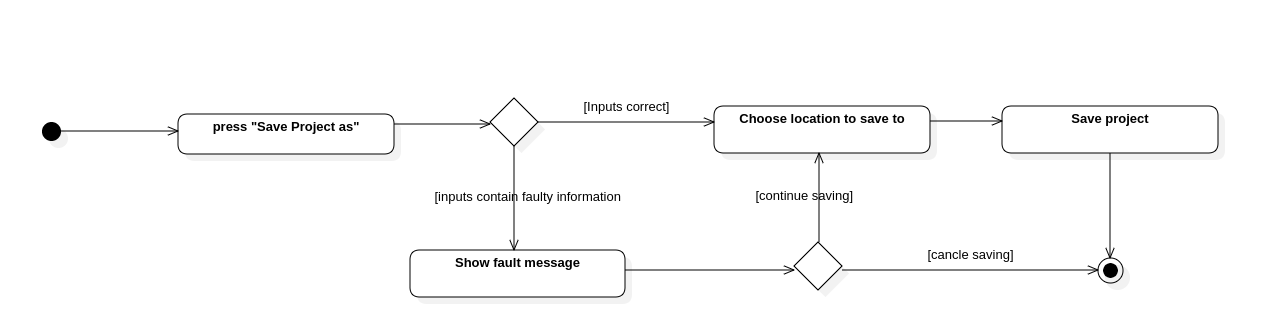
\includegraphics[width=13cm]{entwurf/Entwurf_dokument/img/Alissa/SaveProjectAsAD.png}
    \caption{Aktivitätsdiagramm für Projekt Speichern als}
    \label{ADProkjektSpeichernAls}
\end{figure}
Dafür kann der Nutzer die Option \textit{Save Project As} im Dateimenü wählen. Der Abluf ist mit dem Option \textit{Save project} \ref{ADProjekt Speichern} sehr ähnlich, nur hier kann der Nutzer einen Speicherort mit dem Datei\textendash Dialog wählen.
\\\\
\textbf{\large{CSV Datei exportieren}}
\begin{figure}[H]%
    \centering
    \includegraphics[width=13cm]{entwurf/Entwurf_dokument/img/Alissa/ExportCSVAD.png}
    \caption{Aktivitätsdiagramm für CSV Datei exportieren}
    \label{ad:adExportData}
\end{figure}
Dieser Aktivitätsdiagram \ref{ad:adExportData} beschreibt den Ablauf, wenn der Nutzer die Erhebungsdaten mit den ABleitungen exportieren möchte.
\begin{enumerate}
    \item[1.] Der Nutzer klickt auf \enquote{Export Data} in der Dateimenü
    \item[2.] Wenn es Ableitungen gibt, die fehlerhaft sind, dann wir dem Nutzer eine Fehlermeldung gezeigt. Der Nutzer hat dann die Wahl, den Exportier Vorgang fortzuführen oder abzubrechen.
    \item[3.] Der Nutzer wählt den Speicherort, wo die Daten exportiert werden müssen.
\end{enumerate}

\newpage
\subsection{Attributsmanagement} \label{sec:Attributsmanagement}

Das Attributsmanagement besteht aus fünf verschiedene Funktionen: Ändern, Hinzufügen, Löschen, Importieren und Exportieren von Attributsableitungen. Die Attributsableitungsfunktionen sind im Programm Instanzen der Klasse \classref{FunctionalExpression}, die in einem \textit{dictionary} in der Klasse \classref{Data} des jeweiligen \classref{ProjectSnapshot} hinterlegt sind. Referenziert werden sie über einen vom Nutzer zugewiesenem Namen.

\subsubsection{Änderung einer Attributsableitung} \label{sec:Änderung einer Attributsableitung}
Die Abläufe der Verwaltung dieser Funktionen werden nun beispielhaft anhand eines Sequenzdiagramms (vgl. Abb.~\ref{fig:sd:ChangeDerivativeSequenceDiagram}) beschrieben. Dieses behandelt die Aktion des Nutzers eine bestehende Attributsableitung zu ändern. Vorraussetzung dafür ist, dass mindestens eine Attributsableitung vorhanden ist. Die Sequenzen des Hinzufügens und des Importes funktionieren analog und werden nicht einzeln behandelt.

\begin{figure}[H]%
    \centering
    \includegraphics[width=12cm]{entwurf/Floriane/ChangeDerivative.png}
    \caption{Sequenzdiagramm zur Änderung einer Attributsableitung}
    \label{fig:sd:ChangeDerivativeSequenceDiagram}
\end{figure}

Zuerst wählt der Nutzer eine dargestellte Attributsableitung aus, und ändert den darin vorhandenen mathematischen Ausdruck (Schritt 1). \\\\Das \textit{ColumnWidget} nimmt diese Änderung wahr und ruft im zugewiesenen \textit{DerivativeController} die Funktion \texttt{change(label, expression)} auf (Schritt 2). Dabei ist \texttt{label} ein \textit{String} der den Namen dieser Attributsableitung festlegt und \texttt{expression} die vorgesehene mathematische Formel. Im dritten Schritt wird die Formale validiert und auf Sicherheit überprüft (Schritt 3, vgl Abb. ~\ref{fig:ad:AddDerivative}). Genaueres dazu in ~\ref{sec:Validierung einer Attributsableitung}. \\\\
War die Validierung erfolgreich wird eine Instanz der Klasse \textit{FunctionalExpression} erstellt, die diesen Ausdruck wiedergibt (Schritt 4). Nun ruft der \textit{DerivativeController} über den \textit{Projektmanager} das \textit{ProxyProject} auf (Schritt 5, 6).\\\\
Das \textit{ProxyProject} führt die Funktion \texttt{set\_derivatives(label, new\_derivative)} aus (Schritt 7). Das Funktionsobject \texttt{new\_derivative} wird dabei dem ProxyProjekt übergeben, das alle Funktionen, die auf dem Projekt ausgeführt werden dürfen, übernimmt und dabei bei jeder Änderung einen neuen Snapshot erstellt (vgl Abb. ~\ref{fig:sd:do_operation}, Schritt 8).\\\\
In dem neuen \textit{ProjektSnapshot} werden dann die Änderungen durchgeführt (Schritt 9), indem erst auf die bestehende \textit{Data}-Instanz zugegriffen wird (Schritt 10, 11) und anstelle einer tatsächlichen Änderung eine neue \textit{Data}-Instanz erzeugt wird (Schritt 12, 13), die die geänderte Ableitungsfunktion, sowie alle anderen Daten der vorherigen \textit{Data}-Instanz enthält. Zu beachten ist, dass die Ableitungsfunktionen nicht geändert werden, sondern als eine neue Funktion hinzugefügt werden und die Alte in der neuen Data-Instanz ersetzen. Dies erlaubt dem Nutzer auch die Änderungen, sowie das Löschen und Hinzufügen von Attributsableitungen, rückgängig zu machen. Da die Attributsableitungen in einem \textit{Dictionary} gespeichert werden ist es nicht möglich zwei verschiedene Attributsableitungen mit demselben Namen zu haben.\\\\
Die neue \textit{Data}-Instanz wird dann dem \textit{ProjectSnapshot} zurück gegeben (Schritt 14) und setzt diese in ein neues \textit{Model}-Objekt ein (Schritt 15-17), da auch die \textit{Model}-Instanzen unveränderlich sind um vollständiges Rückgängigmachen zu ermöglichen. Es wird an dieser Stelle das \textit{Model} nicht zurückgegeben (Schritt 18, 19).\\\\
Darauffolgend wird der neue Ausdruck auf inhaltliche Fehler im Kontext des vorhandenen Datensets evaluiert (vgl. Abschnitt ~\ref{sec:Validierung einer Attributsableitung}).\\\\
Nachdem alle Änderungen am Projekt abgeschlossen sind (Schritt 20) wird das Fenster, das die Attributsableitungen zeigt, aktualisiert (vgl. Abschnitt~\ref{sec:Update der Ableitungsübersicht}) und angezeigt.


\subsubsection{Löschen einer Attributsableitung}
Wird alternativ zum Ändern einer Attributsableitung eine Ableitung gelöscht wird anstelle der Methode \texttt{set\_derivative(label: str)} die Methode \texttt{remove\_derivative(label: str)} ausgeführt. Die zu entfernende Attributsableitung wird durch ihren Namen (label) identifiziert und bei der Erstellung eines neuen Data-Objekts (Schritt 13) aus dem Dictionary \texttt{derivatives} entfernt, der alle Attributsableitungen des Projekts enthält, das Objekt wird aber nicht gelöscht oder zerstört, da es sonst aus allen Projektsnapshots entfernt würde und des Rückgängigmachen damit verhindert würde. Der restliche Ablauf ist analog zu Abschnitt -----

\subsubsection{Export einer Attributsableitung} 
Der Export von Attributsableitungen funktioniert analog zu dem der Alternativen (vgl Abschnitt~\ref{sec:Alternativenmanagement}). Die Abläufe unterscheiden sich nur darin, dass statt der Methode \texttt{get\_alternatives(): dict[str, FunctionalExpression]} die Methode \texttt{get\_derivatives(): dict[str, FunctionalExpression]} aufgerufen wird.


\subsubsection{Validierung einer Attributsableitung}\label{sec:Validierung einer Attributsableitung}

Bei der Eingabe eines neuen Ausdrucks als Ableitungsfunktion wird dieser an mehreren Stellen auf Korrektheit überprüft (vgl Abb. ~\ref{fig:ad:AddDerivative}). 

\begin{figure}[H]%
    \centering
    \includegraphics[width=13cm]{entwurf/Floriane/AktivityAddDerivative.png}
    \caption{Attributsableitung Hinzufügen Aktivitätsdiagramm}
    \label{fig:ad:AddDerivative}
\end{figure}
In der Nutzung des Builders zeigt Abb. \ref{fig:ad:AddDerivative} die möglichen Fälle, die auftreten können wenn eine neue Attributsableitung hinzugefügt wird. Der Nutzer klickt auf den '+'-Button und gibt etwas ein. Die Nutzereingabe wird anchließend im \textit{DerivativeController} validiert. Dabei wird die Eingabe nur auf für das Programm gefährliche Inhalte geprüft, nicht auf mathematische Korrektheit. Mögliche Eingaben, die durch diese Validierung abgefangen werden sollen, sind Code, der über einen mathematischen Ausdruck hinaus geht. Insbesondere Eingaben die den Programmablauf gefährden könnten und die Sicherheit beeinträchtigen, wie import Befehle, Endlosschleifen oder Code, der das Programm beendet. Es wird auch überprüft, dass es keine zyklischen Eingaben gibt, also die Ableitung sich nicht selber enthält.

Wird die Eingabe als invalide deklariert, also darf sie nicht von der \texttt{eval()} Funktion eingelesen werden, wird der Vorgang vom Controller beendet. Es wird weder eine \textit{FunktionalExpression}, noch ein neuer \textit{ProjectSnapshot} erstellt. Da sich nichts im Programmzustand geändert hat, wird die Ansicht auch nicht aktualisiert. Es wird nur eine Fehlermeldung angezeigt, dass die Eingabe ungültig war (vgl Abb. \ref{fig:ad:AddDerivative}).
\\\\
Ist die Eingabe valide wird eine \textit{FunctionalExpression} Instanz erstellt und anschließend der Ausdruck mathematisch evaluiert. Diese Evaluierung erfolgt erst nachdem der neue ProjektSnapshot erstellt wurde und somit alle anderen möglichen Variablen im aktuellen Programmzustand feststehen. Bei der mathematischen Evaluierung wird überprüft, ob alle Variablen, die in der Funktion benötigt werden, definiert sind und, ob möglicherweise eine zyklische Abhängigkeit (die neue Attributsableitung hängt über andere Attribute von sich selbst ab) erzeugt wird. 
\\\\\ Die Zyklen werden durch modifizierte Tiefensuche gefunden. Dabei werden die Variablen als Knoten in einem gerichteten Graphen interpretiert. Es existiert eine Kante von Variable A nach Variable B wenn B in der Definition von A existiert. Zur Zyklenprüfung werden die Pfade nach dem Prinzip der Tiefensuche verfolgt, besuchte Knoten werden notiert. Wird ein Knoten mehrfach besucht ist er Teil eines Zyklus. Dadurch kann auch eine Variable in der neuen Funktion als verantwortliche Stelle identifiziert werden.
\\\\ Wird ein Fehler gefunden wird eine Fehlermeldung erzeugt (vgl Abb. \ref{fig:ad:AddDerivative}) und der Funktion angehangen. Diese Fehlermeldung enthält eine Nachricht, die dem Nutzer mitteilt, dass ein Zyklus entsteht, eine Variable nicht definiert ist oder der Ausdruck einen mathematischen Fehler enthält (z.B. Teilen durch 0). Um dem Nutzer die Korrektur zu erleichtern wird die Stelle an der ein Fehler auftritt farbig markiert.\\\\
Wird in beiden Validierungsvorgängen kein Fehler gefunden wird die Funktion ohne eine Markierung hinzugefügt und unter den anderen vorhandenen Ableitungen angezeigt.
\\
\begin{figure}[H]%
    \centering
    \includegraphics[width=12cm]{entwurf/Floriane/GetDerivativeError.png}
    \caption{Sequenzdiagramm zur Fehlererkennung bei Änderung einer Ableitungsfunktionen}
    \label{fig:sd:GetDerivativeError}
\end{figure}

Die Sequenz der Fehlerdarstellung (vgl Abb. \ref{fig:sd:GetDerivativeError}) beginnt nach der Änderung einer Alternative (Schritt 1). Das Label der geänderten Alternative wird an das ProxyProject und damit an den aktuellen \texttt{ProjectSnaphot} durchgegeben (Schritt 2-3). Das Projekt beginnt dann alle Variablen zu sammeln. Erst werden die Prozessvariablen aus der Konfiguration gelesen (Schritt 4-5) und ans Model durchgegeben (Schritt 6). Im Model werden dann die Alternativen mit diesen vereinigt (Schritt 7) an Data weitergegeben (Schritt 8). Data fügt die Ableitungsfunktionen und die Variablen aus den Rohdaten hinzu (Schritt 9) und gibt alle an die neue Funktion weiter (Schritt 10). Dabei wird der neuen Funktion ein Fehlerreport erstellt, und die Fehlerreports der anderen Attributsableitungen aktualisiert (Schritt 11). Der Fehler Report speichert ob der Ausdruck valide ist oder und auftretende Fehlermeldungen und StringMarker, die auf bestimmte Teile des funktionalen Ausdrucks verweisen. Es werden verschiedenen Fehlern auch verschiedene Farben der String Markierung zugewiesen, sodass der Nutzer visuell unterstützt wird in der Fehlerbehebung. Anschließend wird der neue \texttt{ErrorReport} an den Controller (Schritt 12-16) durchgegeben und dieser reicht ihn an die \texttt{View} weiter, die diesen darstellt (Schritt 17).

\subsubsection{Update der Ableitungsübersicht}\label{sec:Update der Ableitungsübersicht}
Die in Abschnitt ~\ref{sec:Änderung einer Attributsableitung} bereits erwähnte Updatesequenz der Ansicht wird in Abbildung ~\ref{fig:sd:UpdateColumnWidgetSequenceDiagram} dargestellt.

\begin{figure}[H]%
    \centering
    \includegraphics[width=13cm]{entwurf/Floriane/UpdateColumnWidget.png}
    \caption{Sequenzdiagramm zur Aktualisierung der Attributsansicht}
    \label{fig:sd:UpdateColumnWidgetSequenceDiagram}
\end{figure}

Der Nutzer interagiert mit der Ansicht, um die Ableitungsfunktionen zu ändern (oder andere Verwaltungsoperationen auszuführen)(Schritt 1). Das Widget gibt die Anfrage an den Controller weiter, dieser führt die angeforderte Funktion aus (Schritt 2 - 3, vgl ~\ref{fig:sd:ChangeDerivativeSequenceDiagram}). Anschließend ruft das Widget die Funktion \texttt{update()} auf, durch die die aktuellen Ableitungsfunktionen aus dem Modell geholt werden (Schritt 4, 5). Über das Vertreterprojekt (Schritt 6 - 8) werden die Funktionen aus der aktuellen Data-Instanz ausgelesen (Schritt 9 - 11) und zurück an das Widget geleitet (Schritt 12 - 16). Das Widget setzt die Funktionen über die von \href{https://doc.qt.io/qt-6/qwidget.html}{PyQt} vorgegebenen Funktionen in die abgebildete Tabelle ein (Schritt 17). Nach dem Update wird die Tabelle angezeigt (Schritt 18).


\newpage
\subsection{Alternativenmanagement}\label{sec:Alternativenmanagement}
Das Alternativmanagement besteht wie das Attributsmanagement aus den folgenden fünf Funktionen: Ändern, Hinzufügen, Löschen, Importieren und Exportieren von Alternativen. Auch Alternativen sind im Programm Instanzen der Klasse \textit{FunctionalExpression}, die in einem \textit{Dictionary} in der Klasse \textit{Model} des jeweiligen \textit{ProjectSnapshot} hinterlegt sind. Referenziert werden sie über einen vom Nutzer zugewiesenem Namen (label).

Da einige Funktionen vergleichbar zu denen aus dem Attributsmanagement sind (vgl. Abschnitt 4.2), werden hier Referenzen angegeben. Die Unterschiede bestehen darin, dass \textit{alternative} anstatt \textit{derivative} genutzt wird und die Klasse Data nicht benötigt wird. Änderungen werden direkt in der Klasse Model durchgeführt.

\subsubsection{Änderung einer Alternative}
Sobald mindestens eine Alternative existiert, kann diese vom Nutzer verändert werden. Dies wird nun mit Hilfe eines Sequenzdiagramms (vgl. Abb.ABC) beschrieben. Die Sequenzen zum Hinzufügen und zum Importieren einer Alternative funktionieren analog und werden nicht einzeln behandelt.
\begin{figure}[H]%
    \centering
    \includegraphics[width=12cm]{entwurf/Entwurf_dokument/img/Kevin/ChangeAlternative.png}
    \caption{Sequenzdiagramm zur Änderung einer Alternative}
    \label{fig:sd:ChangeAlternative}
\end{figure}

Wie man sieht, ist der Ablauf vergleichbar mit der Änderung einer Attributsableitung (vgl. Abschnitt 4.2.1). Die Unterschiede wurden bereits zu Begin beschrieben (vgl. Abschnitt 4.3). Als Beispiel wird statt der Methode \texttt{set\_derivative(label: str, function: FunctionalExpression)} die Methode \texttt{set\_alternative(label: str, function: FunctionalExpression)} aufgerufen.

\subsection{Löschen einer Attributsableitung}
Das Löschen einer Alternative verläuft sehr ähnlich wie das Ändern einer Alternative. Eine genauere Beschreibung befindet sich bereits beim Löschen einer Attributsableitung (vgl. Abschnitt 4.2.2).
Unterschied: Hier wird die Alternative bei der Erstellung eines neuen Model-Objektes (Schritt 11) aus dem Dictionary \texttt{alternatives} entfernt.

\subsection{Export einer Alternative}
Diagramm kommt mit beschreibung.

\subsection{Validierung einer Alternative}

\subsection{Update einer Alternative}

\newpage
\subsection{Konfiguration}
\begin{figure}[H]%
    \centering
    \includegraphics[width=13cm]{entwurf/Entwurf_dokument/img/Michael/sd_change_processing_config.png}
    \caption{Sequenzdiagramm zur Änderung des Verarbeitungskonfigurationstyps}
    \label{fig:sd:ChangeProcessingConfig}
\end{figure}

Der Nutzer hat die Option zwischen verschiedenen Datenverarbeitungsverfahren (\classref{ProcessingConfig}) zu wählen. Dies geschieht im Programm wie folgt:
\begin{enumerate}
    \item[1.] \texttt{QComboBox} empfängt Änderungssinal
    \item[2.] Signal mit neuem Index wird an das \classref{ProcessingWidget} weitergereicht
    \item[3.] Das \classref{ProcessingWidget} gibt dem \classref{ConfigurationController} den Auftrag, das Verarbeitungsverfahren auf den gewünschten Index zu wechseln.
    \item[4.] Der \classref{ConfigurationController} ruft zunächst das aktuelle Projekt auf.
    \item[6.] Der Wechselwunsch wird an das \classref{ProxyProject} weitergegeben.
    \item[7.] Dieses führt den bereits beschriebenen allgemeinen Vorgang \texttt{do\char`_operation} (Abbildung~\ref{fig:sd:do_operation}) mit der \texttt{select\char`_config}-Operation durch.
    \item[9.] In der daraus entstehenden Projektzustandskopie (\classref{ProjectSnapshot}) wird die Änderung in Folge dessen schließlich im \classref{Model} umgesetzt.
    \item[13.] Zurück im \classref{ProcessingWidget} wird von diesem über einen Aufruf der \texttt{update()}-Operation die Benutzeroberfläche aktualisiert.
\end{enumerate}

\begin{figure}[H]%
    \centering
    \includegraphics[width=13cm]{entwurf/Entwurf_dokument/img/Michael/sd_change_processing_settings.png}
    \caption{Sequenzdiagramm zur Änderung der Verarbeitungseinstellungen}
    \label{fig:sd:ChangeProcessingSettings}
\end{figure}

Neben der Auswahl der Verarbeitungsart (siehe Sequenzdiagramm \ref{fig:sd:ChangeProcessingConfig}) hat der Nutzer auch die Möglichkeit diverse Parameter für den durch die Verarbeitungsart gegebenen Algorithmus einzustellen. Hierzu trägt er die gewünschten Werte in eine Tabelle in der Benutzeroberfläche ein. Daraus entsteht folgende Sequenz:

\begin{enumerate}
    \item[1.] Der Nutzer löst mit der Änderung einer Tabellenzelle das \emph{PyQt}-Signal \texttt{setCurentItem(item)} aus. Das Widget bemerkt, dass eine Änderung vorgenommen wurde.
    \item[2.] Die Änderungsinformation wird an das übergeordnete \classref{ProcessingWidget} weitergegeben.
    \item[3.] Von dort aus wird der dafür zuständige \classref{ConfigurationController} beauftragt, die Änderung ins Model zu übertragen.
    \item[4.] Zunächst fragt dieser den Index der aktuell ausgewählten \classref{ProcessingConfig} (siehe auch \ref{fig:sd:ChangeProcessingConfig}) vom \classref{ProxyProject} ab.
    \item[5.] Dort wird der Index wiederum von der aktuell gültige Projektreferenz (\classref{ProjectSnapshot}) angefragt.
    \item[8.] Nachdem der Index der aktuellen \classref{ProcessingConfig} zurück im \text{ConfigurationController} ist, fragt dieser nun die bisher getätigten Einstellungen in Form einer Kopie vom \classref{ProxyProject} ab.
    \item[9.] Dies wird wie ebenfalls direkt an den aktuellen \classref{ProjectSnapshot} weitergegeben.
    \item[12.] Nach erhalt der Einstellungen verändert der Controller die erhaltene Kopie entsprechend der umzusetzenden Benutzereingaben (\texttt{n\char`_settings}). Dieses wird dem \classref{ProxyProject} nun zur Änderung aller Einstellungen vollständig übergeben.
    \item[13.] Im \classref{ProxyProject} wird hierzu der bereits beschriebenen allgemeinen Vorgang \texttt{do\char`_operation} (Abbildung~\ref{fig:sd:do_operation}) mit der \texttt{set\char`_config\char`_settings}-Operation durchgeführt.
    \item[15.] Der aktuelle \classref{ProjectSnapshot} erhält den Änderungsauftrag.
    \item[16.] Dieser gibt ihn an die jeweilige Konfigurationsklasse (wie \classref{SimpleProcessingConfig}) weiter.
    \item[22.] Zurück im \classref{ProcessingWidget} wird von diesem über einen Aufruf der \texttt{update()}-Operation die Benutzeroberfläche aktualisiert.
\end{enumerate}

\subsection{Evaluation}
Hier befindet sich das eigentliche Ziel des Nutzers, nämlich die Schätzung der Parameter, welche in den Alternativen hinterlegt sind. \\
Abhängig von der Berechnungsmethode in der \classref{ProcessingConfig} können hier weitere Werte aus der Berechnung ausgegeben und visualisiert werden.

\subsubsection{Ausführen einer Evaluation}
\begin{figure}[H]%
    \centering
    \includegraphics[width=13cm]{entwurf/Entwurf_dokument/img/Damian/Berechnung durchführen.png}
    \caption{Sequenzdiagramm zur Ausführung der Evaluation}
    \label{fig:sd:CalculateEvaluation}
\end{figure}

Für die Evaluierung muss mindestens eine Alternative im Projekt hinterlegt worden sein (vgl. Abb. \ref{fig:sd:ChangeAlternative}).\\
\begin{enumerate}
    \item [1. -- 2.] Zum Starten der Berechnung drückt der Nutzer auf den Button \fbox{\texttt{Calculate Evaluation}}. Daraufhin wird die entsprechende Methode in dem \classref{EvaluationWidget} gestartet.
    \item [3.] Um eine laufende Berechnung vom Nutzer abbrechbar zu machen, wird ein \texttt{Thread} erzeugt.
    \item [4 -- 10] Der neue \texttt{Thread} kapselt den Aufruf zum \classref{EvaluationController} und startet die Berechnung.
    \item [] Nach Erzeugen des Threads erstellt das \classref{EvaluationWidget} ein neues Fenster, welches den Nutzer informiert, dass die Berechnung ausgeführt wird. Dieses dient dazu, den Rest der Applikation für Nutzereingaben zu sperren. \\
    Das Fenster ermöglicht zudem über den Button \fbox{\texttt{Abort}} eine Möglichkeit die Berechnung abzubrechen (\texttt{alt: [abort]}). Daraufhin wird der laufende \texttt{Thread} terminiert (12) und das neue Fenster geschlossen. Ein \texttt{update()}-Aufruf (siehe Abb. \ref{fig:sd:UpdateEvaluationWidget}) muss nach Abbruch erfolgen, da potentiell bereits ein neuer \classref{ProjectSnapshot} angelegt wurde, der \texttt{Thread} jedoch noch nicht komplett zurückkehrte. \\
    \item [18.] Wartet der Nutzer auf das Ende der Berechnung ab (\texttt{alt: [wait]}), so wird nach erfolgreichem Ablauf des erzeugten \texttt{Threads} anschließend ein \texttt{update()}-Aufruf gestartet. Damit werden die neuen Ergebnisse in das \classref{EvaluationWidget} geladen und angezeigt..
\end{enumerate}

\begin{figure}[H]%
    \centering
    \includegraphics[width=13cm]{entwurf/Entwurf_dokument/img/Damian/EvaluationWidget.update().png}
    \caption{Sequenzdiagramm zur Ausführung der Evaluation}
    \label{fig:sd:UpdateEvaluationWidget}
\end{figure}

Für jeden \texttt{update()}-Aufruf wird zweimal auf den \classref{EvaluationController} zugegriffen. \\
Dabei werden separat auf die Ergebnisse der Evaluation (2 - 9) und die hinterlegten Schwellwerte (10 - 17) zugegriffen. \\
Die Werte werden anschließend gemeinsam im \classref{EvaluationWidget} visualisiert.

\subsubsection{Optimieren des Modells}
\begin{figure}[H]%
    \centering
    \includegraphics[width=13cm]{entwurf/Entwurf_dokument/img/Michael/sd_optimize_model.png}
    \caption{Sequenzdiagramm der Modelloptimierung}
\end{figure}

Nachdem aus einem definierten diskreten Wahlmodell durch Anwendung eines Verarbeitungsverfahrens ein Ergebnis berechnet wurde, besteht bei manchen Verfahren die Möglichkeit, das zugrunde gelegte Wahlmodell aufgrund des Ergebnisses zu optimieren. Bei Auswertungen, bei denen eine varrierte Parameterschätzung (\classref{VariedProcessingConfig}) verwendet wurde, geschieht dies durch Festlegung der variierten Parameter auf Werte, die im Ergebnis die höchsten Signifikanzen geliefert haben. Nachdem der Nutzer mit der entsprechenden Schaltfläche das Modell optimieren lässt, entsteht folgende Sequenz:

\begin{enumerate}
    \item[1.] Der dafür zuständige Knopf der Benutzeroberfläche erhält das \emph{PyQt}-Signal \texttt{clicked}.
    \item[2.] Der Optimierungswunsch wird an das übergeordnete \classref{EvaluationWidget} weitergegeben.
    \item[3.] Von dort aus wird die Operation an den dafür zuständige \classref{ConfigurationController} weitergegeben.
    \item[4.] Der \classref{ConfigurationController} ruft zunächst das aktuelle \classref{ProxyProjekt} auf.
    \item[6.] Das \classref{ProxyProjekt} erhält vom \classref{ConfigurationController} den Optimierungsauftrag.
    \item[7.] Dieses führt den bereits beschriebenen allgemeinen Vorgang \texttt{do\char`_operation} (Abbildung~\ref{fig:sd:do_operation}) mit der \texttt{optimize\char`_model}-Operation durch.
    \item[9.] In der daraus entstehenden Projektzustandskopie (\classref{ProjectSnapshot}) wird die Optimierung an die Evaluation.
\end{enumerate}

\subsubsection{Exportieren der Ergebnisse}
\begin{figure}[H]%
    \centering
    \includegraphics[width=13cm]{entwurf/Entwurf_dokument/img/Damian/Ergebnisse exportieren.png}
    \caption{Sequenzdiagramm zum Export der Ergebnisse}
    \label{fig:sd:ExportEvaluation}
\end{figure}


Möchte der Nutzer die berechnete Evaluation exportieren, so wird nach Betätigung des Buttons \fbox{\texttt{Export}} ein neues \classref{FileManagementWindow} geöffnet (1 -- 3). \\
Dieses lässt den Nutzer den Dateipfad für die erstellte Datei wählen. Die Interaktion erfolgt dabei über bereits implementierte Methoden, die das \classref{FileManagementWindow} aus dem externen Paket \texttt{PyQt} erbt (4 -- 8). \\
Der übergebene Pfad, welcher den Dateinamen enthält, wird anschließend an den \classref{EvaluationController} übergeben. Dieser holt sich das \texttt{pandas.DataFrame}-Objekt, welches in der \classref{Evaluation} hinterlegt ist und führt darauf den Export aus (9 -- 21).


\subsubsection{Schwellwerte für die Visualisierung konfigurieren}
Nach Berechnung der Evaluation (siehe Abb. \ref{fig:sd:CalculateEvaluation}) können den Spalten vom Nutzer Schwellwerte zugeteilt werden. Diese haben eine Auswirkung auf die farbliche Visualisierung der Ergebnistabelle.
\begin{figure}[H]%
    \centering
    \includegraphics[width=13cm]{entwurf/Entwurf_dokument/img/Damian/Schwellwerte konfigurieren.png}
    \caption{Sequenzdiagramm zur Konfigurierung der Schwellwerte}
    \label{fig:sd:ChangeThresholds}
\end{figure}

\begin{enumerate}
    \item [1.] Nachdem die Berechnungen ausgeführt wurden und dargestellt sind, kann der Nutzer auf den Button \fbox{\texttt{View Options}} drücken.
    \item [3. -- 10.] Dieser sendet das Signal an das \classref{EvaluationWidget}. Es soll ein neues Fenster \classref{ThresholdWindow} erzeugt werden, welches die gespeicherten Schwellwerte anzeigt und verändern lässt. Dazu müssen die Schwellwerte erst aus dem \classref{ProjectSnapshot} geholt werden.
    \item [12.] Das neue \classref{ThresholdWindow} ermöglicht das Verändern der Schwellwerte in der Ergebnistabelle. 
    \item [13. -- 24.] Änderungen sollen gemeinsam in einem neuen \classref{ProjectSnapshot} gespeichert werden. Beim Aufruf sperrt das Fenster dem Nutzer also den Zugriff auf den Rest der Anwendung, damit es gesichert zu keinen Synchronitätsfehlern kommen kann. \\ Änderungen können über einen Button \fbox{\texttt{Cancel}} rückgängig gemacht werden und das Fenster wird geschlossen. Nach Anwendung der Änderung über den Button \fbox{\texttt{Apply}}, werden die neuen Schwellwerte in einem neuen \classref{ProjectSnapshot} hinterlegt. 
    \item [25.] Das \classref{EvaluationWidget} lädt die Visualisierung daraufhin neu (siehe Abb. \ref{fig:sd:UpdateEvaluationWidget}).
    \item [27.] Anschließend wird das \classref{ThresholdWindow} geschlossen.
\end{enumerate}

\section{Datenhaltung}

Der Model Builder speichert fünf verschiedene Ergebnisse: Alternativen, Attributsableitungen, Signifikanzen und Parameter, sowie die CSV-Dateien mit den zugrunde liegenden Umfragedaten und berechneten Attributen. Dabei werden Alternativen und Attributsableitungen im JSON-Format gespeichert, sodass sie in anderen Projekten widerverwertet werden können.

\subsection{Alternativen}
Die Alternativen werden als JSON-Dateien mit ihren Attributen 'label' und 'functional\_expression' gespeichert. Zusätzlich wird ebenfalls das Erstellungsdatum gespeichert.
\texttt{\begin{tabbing}
    \{\\
    \qquad"{}label": <str>,\\
    \qquad"{}functional\char`_expression": \{\\
    \qquad\qquad"{}expression": <str>\\
    \qquad\}\\
    \}
\end{tabbing}}

Das Label wird als String gespeichert und dient der Unterscheidung der einzelnen Alternativen. Das Objekt der FunctionalExpression, das im Builder verwendet wird, wird unter 'functional\_expression' als Objekt mit seinen Attributen gespeichert. In diesem befindet sich die von Python evaluierbare Funktion unter "expression", inklusive möglicher nicht-behobener Fehler.

\subsection{Attributsableitungen}
Die Attributsableitungen werden ebenfalls separat als Funktion in einer JSON-Datei gespeichert. In den Dateien befinden sich die Schlüssel 'label' und 'functional\_expression'. Der Schlüssel 'label' enthält den gewählten Namen der Attribtusableitung, und 'functional\_expression' enthält das Objekt aus dem Projekt im JSON-Format. Dieses enthält den Funktionasausdruck als String unter dem Schlüssel 'expression'.
\texttt{\begin{tabbing}
    \{\\
    \qquad"{}label": <str>,\\
    \qquad"{}functional\char`_expression": \{\\
    \qquad\qquad"{}expression": <str>\\
    \qquad\}\\
    \}
\end{tabbing}}

\subsection{Umfragedaten und berechnete Attribute}
Die Umfragedaten werden auf Wunsch mit den berechneten Attributen in einer gemeinsamen CSV-Datei gespeichert. 

Dabei entsprechen die Zeilen jeweils einer berechneten Attributsableitung. Die Spaltenüberschriften entsprechen den gesetzten Namen der Attributsableitungen. 

\subsection{Parameter und Signifikanzen}
Die berechneten Parameter und Signifikanzen werden in einer CSV-Datei unter ihrem zugehörigen Variablen Namen gespeichert. Jede Zeile entspricht einer Variable aus den Nutzenfunktionen.

Die Spalten enthalten die aus der Berechnung durch Biogeme hervorgehenden Parameter. Um die Nachvollziehbarkeit der Berechnungen zu gewährleisten, und dem Nutzer alle für ihn  möglicherweise interessanten Informationen über die Berchnung zu geben, werden in der Parameter Datei alle von Biogeme berechneten Parameter angegeben. Dabei sind mindestens die Spalte 'Value' für den berechneten Wert, sowie die Spalte "stdErr" für die Standardabweichung des jeweiligen Wertes vorhanden.

Die erste Spalte in der Tabelle enthält die durch die Nutzenfunktoinen festgelegten Variablennamen zur Zuordnung der Werte.


\section{Änderungen im Pflichtenheft}
In dem Entwurf sind Änderungen am Pflichtenheft vorgenommen worden. Es wurden Wunschkriterien, sowie selbst gesetzte Maßstäbe angepasst.

\subsection{EditMenu}
Das Bearbeitungsmenu aus Abbildung 8.8 im Pflichtenheft bezieht sich nur in den Funktionen 'undo' und 'redo' auf das gesamte Projekt. Die restlichen Funktionen beziehen sich auf den abgebildeten bzw. eingegeben Text, aber nicht die Objekte, die diesem unterliegen.

\subsection{Speicherung}
Anstelle einer zeitlich geregelten regelmäßigen Speicherung alle 60 Sekunden (vgl 6.1 Projektdaten im Pflichtenheft) wird das gesamte Projekt nach jedem Bearbeitungsschritt gespeichert, bei dem ein neuer Projektsnapshot erstellt wird.


\section{Anhang}
\begin{figure}[H]%
    \centering
    \includegraphics[width=13cm]{entwurf/Entwurf_dokument/img/KlassendiagrammAlles.png}
    \caption{Vollständiges Klassendiagramm}
    \label{fig:CompleteClassDiagram}
\end{figure}



\printglossary
\end{document}